
% $Author: oscar $
% $Translation: martial $
% $Date: Wed Oct 10 17:20:28 CEST 2007 $
% $Revision: 12715 $
%=================================================================
% translated by Martial.Boniou@ifrance.com start: (Fri, 28 Sep 2007)
% relecture par Rene Mages : Thu Dec 20 12:13:40 2007
% relecture par Martial : Sat Dec 29 16:06:42 CET 2007
% relecture par Rene Mages : Thr Jan 10 17:17:17 2008
%% j'ai enleve les 'transmissions de messages': il ne reste que 'envoi
%% de messages'; j'ai remplace 'envoi sur super/self' par 'envoi a
%% ...'; j'ai remplace '\lct{}' par '\ct{}' quand possible
%
% adaptation pour PBE - martial - Thu Sep 10 20:18:24 CEST 2009 
% relecture par Rene Mages : Tue Jan 12 17:17:17 2010
% relecture par Rene Mages : Tue Aug  8 17:17:17 2010
% relecture par Rene Mages : Mon Apr 11 17:17:17 2011
% relecture par Rene Mages : Wed May  4 17:17:17 2011
% $Author: oscar $ $Date: 2009-08-28 11:02:05 +0200 (Fri, 28 Aug 2009) $ $Revision: 28659 $
% sync avec la version: 29660
%=================================================================
\ifx\wholebook\relax\else
% --------------------------------------------
% Lulu:
	\documentclass[a4paper,10pt,twoside]{book}
	\usepackage[
		papersize={6.13in,9.21in},
		hmargin={.75in,.75in},
		vmargin={.75in,1in},
		ignoreheadfoot
	]{geometry}
	% $Author$ Martial
% $Date$ Wed Oct 10 13:34:55 CEST 2007
% $Revision$ source: SBE 12715 
% Last Changed Date: 2007-10-08 21:32:45 +0200 (Mon, 08 Oct 2007)
% sync avec la version: 29516 - Mon Nov 16 19:12:49 2009
%=============================================================
% NB: documentclass must be set in main document.
% Allows book to be generated in multiple formats.
%=============================================================
%:Packages
\usepackage[french]{babel}
\usepackage[T1]{fontenc}  %%%%%% really important to get the code directly in the text!
\usepackage{lmodern}
%\usepackage[scaled=0.85]{bookmanx} % needs another scale factor if used with \renewcommand{\sfdefault}{cmbr}
\usepackage{palatino}
\usepackage[scaled=0.85]{helvet}
\usepackage{microtype}
\usepackage{graphicx}
\usepackage{theorem}
\usepackage[utf8]{inputenc}
% ON: pdfsync breaks the use of p{width} for tabular columns!
\ifdefined\usepdfsync\usepackage{pdfsync}\fi % Requires texlive 2007
%=============================================================
%:More packages
%Stef should check which ones are used!
%\usepackage{picinpar}
%\usepackage{layout}
%\usepackage{color}
%\usepackage{enum}
%\usepackage{a4wide}
% \usepackage{fancyhdr}
\usepackage{ifthen}
\usepackage{float}
\usepackage{longtable}
\usepackage{makeidx}
\usepackage[nottoc]{tocbibind}
\usepackage{multicol}
\usepackage{booktabs}	% book-style tables
\usepackage{topcapt}	% enables \topcaption
\usepackage{multirow}
\usepackage{tabularx}
%\usepackage[bottom]{footmisc}
\usepackage{xspace}
%\usepackage{abbrevs} % vf only (for \newname command)
\usepackage{alltt}
\usepackage{amssymb,textcomp}
\usepackage[usenames,dvipsnames]{color}
%\usepackage{colortbl}
\usepackage[hang]{subfigure}\makeatletter\def\p@subfigure{\thefigure\,}\makeatother
\usepackage{rotating}
\usepackage{enumitem}	% apb: allows more control over tags in enumerations
\usepackage{verbatim}     % for comment environment
\usepackage{varioref}	% for page references that work
\labelformat{footnote}{\thechapter--#1} % to distinguish citations from jurabib
\usepackage{needspace}
\usepackage{isodateo} % enable \isodate
\usepackage[newparttoc]{titlesec}
\usepackage{titletoc}
\usepackage{eurosym}
\usepackage{wrapfig}
\usepackage{import}

\usepackage[
	super,
	citefull=first,
	authorformat={allreversed,and},
	titleformat={commasep,italic}
]{jurabib} % citations as footnotes
\usepackage[
	colorlinks=true,
	linkcolor=black,
	urlcolor=black,
	citecolor=black
]{hyperref}   % should come last
%=============================================================
%:PDF version
\pdfminorversion=3 % Set PDF to 1.3 for Lulu
%=============================================================
%:URL style
\makeatletter

\def\url@leostyle{%
  \@ifundefined{selectfont}{\def\UrlFont{\sf}}{\def\UrlFont{\sffamily}}}
% ajouter par Martial pour \traduit (met une dague dans les \doublebox
\def\thempfootnote{\fnsymbol{mpfootnote}}

\makeatother
% Now actually use the newly defined style.
\urlstyle{leo}
%=============================================================
%:Booleans
\newboolean{lulu} % version lulu
\setboolean{lulu}{false}
\newboolean{deployment} % version de déploiement
\setboolean{deployment}{false}  % true pour enlever les couleurs et
                                % annotations de traduction
\newcommand{\ifluluelse}[2]{\ifthenelse{\boolean{lulu}}{#1}{#2}}
\newcommand{\ifdeploy}[1]{\ifthenelse{\boolean{deployment}}{#1}{}}      % vf only
%=============================================================
%:Names
\newcommand{\SUnit}{SUnit\xspace}
\newcommand{\sunit}{SUnit\xspace}
\newcommand{\xUnit}{$x$Unit\xspace}
\newcommand{\JUnit}{JUnit\xspace}
%\newcommand{\XP}{eXtreme Programming\xspace}
\newcommand{\st}{Smalltalk\xspace}
\newcommand{\pharo}{Pharo\xspace} % utilisé \pharo et non \Pharo
\newcommand{\sqsrc}{SqueakSource\xspace}
\newcommand{\sqmap}{SqueakMap\xspace}
\newcommand{\squeak}{Squeak\xspace}
%\newcommand{\sbe}{\url{scg.unibe.ch/SBE}\xspace}
%\newcommand{\sbe}{\url{squeakbyexample.org}\xspace}
\newcommand{\sbe}{\url{http://SqueakByExample.org}\xspace}
% pharo
\newcommand{\pharoweb}{\url{http://pharo-project.org}\xspace}
\newcommand{\pbe}{\url{http://PharoByExample.org}\xspace}
% pharo-french
\newcommand{\ppe}{\url{http://PharoByExample.org/fr}\xspace} % ATTENDRE - à définir
% squeak-fr: adresse de la version francaise
\newcommand{\spe}{\url{http://SqueakByExample.org/fr}\xspace}
\newcommand{\sba}{\url{http://SquareBracketAssociates.org}\xspace}
% squeak-fr: ajout de la \squeakdev pour eviter les problemes de
% changements d'url rencontres dans la VO:
\newcommand{\squeakdev}{\url{http://www.squeaksource.com/ImageForDevelopers}\xspace} %ou
%\newcommand{\squeakdev}{\url{squeak.ofset.org/squeak-dev}\xspace}
\newcommand{\bam}{\lct{Bounc\-ing\-Atoms\-Morph}\xspace} % REVOIR
%=============================================================
%:Markup macros for proof-reading
\usepackage[normalem]{ulem} % for \sout
\usepackage{xcolor}
\newcommand{\ra}{$\rightarrow$}
\newcommand{\ugh}[1]{\textcolor{red}{\uwave{#1}}} % please rephrase
\newcommand{\ins}[1]{\textcolor{blue}{\uline{#1}}} % please insert
\newcommand{\del}[1]{\textcolor{red}{\sout{#1}}} % please delete
\newcommand{\chg}[2]{\textcolor{red}{\sout{#1}}{\ra}\textcolor{blue}{\uline{#2}}} % please change
%=============================================================
%:Editorial comment macros
%\newcommand{\nnbb}[2]{
%    \fbox{\bfseries\sffamily\scriptsize#1}
%    {\sf\small$\blacktriangleright$\textit{#2}$\blacktriangleleft$}
%   }
\newcommand{\yellowbox}[1]{\fcolorbox{gray}{yellow}{\bfseries\sffamily\scriptsize#1}}
\newcommand{\triangles}[1]{{\sf\small$\blacktriangleright$\textit{#1}$\blacktriangleleft$}}
\newcommand{\nnbb}[2]{\yellowbox{#1} \triangles{#2}}
\newcommand{\fix}{\yellowbox{À CORRIGER!}}
\newcommand{\here}{\yellowbox{CONTINUE ICI!}}

% macros éditeurs/traducteurs
\newcommand{\ab}[1]{\nnbb{Andrew}{#1}} % Black
\newcommand{\sd}[1]{\nnbb{St\'{e}f}{#1}} % Ducasse
\newcommand{\md}[1]{\nnbb{Marcus}{#1}} % Denker
\newcommand{\on}[1]{\nnbb{Oscar}{#1}} % Nierstrasz
\newcommand{\damien}[1]{\nnbb{Damien}{#1}} % Pollet
\newcommand{\lr}[1]{\nnbb{Lukas}{#1}} % Renggli
\newcommand{\orla}[1]{\nnbb{Orla}{#1}} % Greevy
\newcommand{\alex}[1]{\nnbb{Alex}{#1}} % Bergel
\newcommand{\alx}[1]{\nnbb{Alex}{#1}} % Bergel
\newcommand{\dr}[1]{\nnbb{David}{#1}} % Roethlisberger
\newcommand{\ja}[1]{\nnbb{Jannik}{#1}} % Laval
\newcommand{\jr}[1]{\nnbb{Jorge}{#1}} % Ressia
\newcommand{\fp}[1]{\nnbb{Fabrizio}{#1}} % Perin
\newcommand{\michael}[1]{\nnbb{Michael}{#1}} % Davies
\newcommand{\ew}[1]{\nnbb{Erwann}{#1}} % Wernli
\newcommand{\mb}[1]{\nnbb{Martial}{#1}} % Boniou
\newcommand{\hw}[1]{\nnbb{Hernan}{#1}} % Wilkinson
%=============================================================
%:Abbreviation macros
\newcommand{\ie}{\emph{c-\`a-d.}\xspace}
\newcommand{\cad}{\emph{c-\`a-d.}\xspace}
%\newcommand{\eg}{\emph{e.g.},\xspace}
\newcommand{\eg}{\emph{par ex.},\xspace}
\newcommand{\parex}{\emph{par ex.},\xspace}
\newcommand{\etc}{etc\xspace}
%=============================================================
%:Cross reference macros

% [squeak-fr] martial: remarquez les articles devant les noms
\newcommand{\charef}[1]{le chapitre~\ref{cha:#1}\xspace}
% note de martial: utilise dans chapitre Syntax.tex: a redefinir
\newcommand{\charefs}[2]{les chapitres~\ref{cha:#1} et \ref{cha:#2}\xspace}
\newcommand{\secref}[1]{la section~\ref{sec:#1}\xspace}
\newcommand{\figref}[1]{la figure~\ref{fig:#1}\xspace}
\newcommand{\Figref}[1]{La figure~\ref{fig:#1}\xspace}
\newcommand{\appref}[1]{l'annexe~\ref{app:#1}\xspace}
\newcommand{\tabref}[1]{la table~\ref{tab:#1}\xspace}
% defini pour le chapitre Messages.tex
\newcommand{\Tabref}[1]{La table~\ref{tab:#1}\xspace}
\newcommand{\faqref}[1]{la FAQ~\ref{faq:#1}, p.~\pageref{faq:#1}\xspace}

% [pharo] ajout
\newcommand{\chalabel}[1]{\label{cha:#1}}
\newcommand{\seclabel}[1]{\label{sec:#1}}
\newcommand{\figlabel}[1]{\label{fig:#1}}
\newcommand{\tablabel}[1]{\label{tab:#1}}
\newcommand{\rulelabel}[1]{\label{rule:#1}}
\newcommand{\eglabel}[1]{\label{eg:#1}}
\newcommand{\scrlabel}[1]{\label{scr:#1}}
\newcommand{\mthlabel}[1]{\label{mth:#1}}
\newcommand{\clslabel}[1]{\label{cls:#1}}
\newcommand{\faqlabel}[1]{\label{faq:#1}}

% APB: I removed trailing \xspace commands from these macros because
% \xspace mostly doesn't work.  If you want a space after your
% references, type one!
% ON: xspace has always worked just fine for me!  Please leave them in.
%
\newcommand{\ruleref}[1]{\ref{rule:#1}\xspace}
%
\newcommand{\egref}[1]{exemple~\ref{eg:#1}\xspace}
\newcommand{\Egref}[1]{Exemple~\ref{eg:#1}\xspace}
%
\newcommand{\scrref}[1]{script~\ref{scr:#1}\xspace}
\newcommand{\Scrref}[1]{Script~\ref{scr:#1}\xspace}
% t = the
\newcommand{\tscrref}[1]{le script~\ref{scr:#1}\xspace}
\newcommand{\Tscrref}[1]{Le script~\ref{scr:#1}\xspace}
%
\newcommand{\mthref}[1]{m\'ethode~\ref{mth:#1}\xspace}
\newcommand{\mthsref}[1]{m\'ethodes~\ref{mth:#1}\xspace}
\newcommand{\Mthref}[1]{M\'ethode~\ref{mth:#1}\xspace}
\newcommand{\tmthref}[1]{la m\'ethode~\ref{mth:#1}\xspace}
\newcommand{\Tmthref}[1]{La m\'ethode~\ref{mth:#1}\xspace}
%
\newcommand{\clsref}[1]{classe~\ref{cls:#1}\xspace}
\newcommand{\tclsref}[1]{la classe~\ref{cls:#1}\xspace}
\newcommand{\Tclsref}[1]{La classe~\ref{cls:#1}\xspace}
%=============================================================
%:Menu item macro
% for menu items, so we can change our minds on how to print them! (apb)
\definecolor{lightgray}{gray}{0.89}
\newcommand{\menu}[1]{{%
	\setlength{\fboxsep}{0pt}%
	\colorbox{lightgray}{{{\upshape\sffamily\strut \,#1\,}}}}}
\newcommand{\link}[1]{{%
 \fontfamily{lmr}\selectfont
  {\upshape{\sffamily \underline{#1}}}}}
% \newcommand{\menu}[1]{{%
% 	\fontfamily{lmr}\selectfont
% 	\upshape\textlangle{\sffamily #1}\textrangle}}
% For submenu items:
\newcommand{\go}{\,$\triangleright$\,}
% \newcommand{\go}{\,$\blacktriangleright$\,}
% For keyboard shortcuts:
%\newcommand{\short}[1]{\mbox{$\langle${\sc CMD}$\rangle$-#1}\xspace}
\newcommand{\short}[1]{\mbox{{\sc cmd}\hspace{0.08em}--\hspace{0.09em}#1}\xspace}
% For buttons:
\newcommand{\button}[1]{{%
	\setlength{\fboxsep}{0pt}%
	\fbox{{\upshape\sffamily\strut \,#1\,}}}}
\newcommand{\toolsflap}{l'onglet \textit{Tools}}
%=============================================================
%:Mouse clicks % REVOIR * % CHANGE
% [martial: ce sont des verbes] ==BOUTONS==
\newcommand{\clickbtn}{clic\xspace} % inutilisé
\newcommand{\actclickbtn}{clic d'action\xspace} % inutilisé
\newcommand{\metaclickbtn}{meta-clic\xspace} % inutilisé
\newcommand{\click}{cliquer\xspace} % RED = click
\newcommand{\actclick}{cliquer avec le bouton d'action\xspace} % YELLOW = action-click
\newcommand{\metaclick}{meta-cliquer\xspace} % BLUE = meta-click
\newcommand{\Click}{Cliquer\xspace} % RED = click
\newcommand{\Actclick}{Cliquer avec le bouton d'action\xspace} % YELLOW = action-click
\newcommand{\Metaclick}{Meta-cliquer\xspace} % BLUE = meta-click
\newcommand{\clickant}{cliquant\xspace} % RED = click
\newcommand{\actclickant}{cliquant avec le bouton d'action\xspace} % YELLOW = action-click
\newcommand{\metaclickant}{meta-cliquant\xspace} % BLUE = meta-click
\newcommand{\clickz}{cliquez\xspace} % RED = click
\newcommand{\actclickz}{cliquez avec le bouton d'action\xspace} % YELLOW = action-click
\newcommand{\metaclickz}{meta-cliquez\xspace} % BLUE = meta-click
\newcommand{\Clickz}{Cliquez\xspace} % RED = click
\newcommand{\Actclickz}{Cliquez avec le bouton d'action\xspace} % YELLOW = action-click
\newcommand{\Metaclickz}{Meta-cliquez\xspace} % BLUE = meta-click
%=============================================================
%:ToSh macros
\newboolean{tosh}
\setboolean{tosh}{false}
\newcommand{\iftoshelse}[2]{\ifthenelse{\boolean{tosh}}{#1}{#2}}
%=============================================================
%:ToSh colors
%\newcommand{\highlightcolor}{\color{blue!65}}
%\newcommand{\boxcolor}{\color{gray!25}}
\newcommand{\highlight}[1]{\textcolor{blue!65}{#1}}
%\newcommand{\codecolor}{\color{blue!65}}
%%\setlength{\fboxrule}{2pt}
%\newcommand{\asPict}[1]{%
%	{\Large\highlight{#1}}}
%=============================================================
%:Reader cues (do this)
%
% Indicate something the reader should try out.
% \newcommand{\dothisicon}{\raisebox{-.5ex}{
\includegraphics[width=1.4em]{squeak-logo}}}
\iftoshelse{
	\usepackage{marginnote}
		\renewcommand*{\marginfont}{\footnotesize}
	\newcommand{\vartriangleout}{\ifthenelse{\isodd{\thepage}}{\vartriangleright}{\vartriangleleft}}
	\newcommand{\dothisicon}{\fcolorbox{blue!65}{white}{\highlight{$\vartriangleout$}}}
	\newcommand{\dothis}[1]{%
		\noindent\par\noindent
		{\reversemarginpar
			\marginnote{\fcolorbox{blue!65}{white}{\highlight{$\vartriangleout$}}}}
		%\MarginLabel{do this}
		\noindent\emph{#1}
		\nopagebreak}
}{
	\newcommand{\dothisicon}{\raisebox{-.5ex}{
\includegraphics[height=1.2em]{pharo}}}
	\newcommand{\dothis}[1]{%
		\medskip
		\noindent\dothisicon
		\ifx#1\empty\else\quad\emph{#1}\fi
		\par\smallskip\nopagebreak}
}
%===> NEW VERSION <===
% NB: To use this in an individual chapter, you must set:
%\graphicspath{{figures/} {../figures/}}
% at the head of the chapter.  Don't forget the final /
%=============================================================
%:Reader hints (hint)
%
% Indicates a non-obvious consequence 
\newcommand{\hint}[1]{\vspace{1ex}\noindent\fbox{\textsc{Astuce}} \emph{#1}}
%=================================================================
% graphics for Morphic handles
\newcommand{\grabHandle}{\raisebox{-0.2ex}{
\includegraphics[width=1em]{blackHandle}}}
\newcommand{\moveHandle}{\raisebox{-0.2ex}{
\includegraphics[width=1em]{moveHandle}}}
\newcommand{\debugHandle}{\raisebox{-0.2ex}{
\includegraphics[width=1em]{debugHandle}}}
% squeak-fr (added for Morphic handles)
\newcommand{\rotateHandle}{\raisebox{-0.2ex}{
\includegraphics[width=1em]{rotateHandle}}}
\newcommand{\viewerHandle}{\raisebox{-0.2ex}{
\includegraphics[width=1em]{viewerHandle}}} % A RETIRER (les eToys ne sont plus)
% squeak-fr (add cloverHandle to use \clover in QuickTour.tex as alias
% todo 

%=============================================================
%:Highlighting Important stuff (doublebox)
%
% From Seaside book ...
\newsavebox{\SavedText}
\newlength{\InnerBoxRule}\setlength{\InnerBoxRule}{.75\fboxrule}
\newlength{\OuterBoxRule}\setlength{\OuterBoxRule}{1.5\fboxrule}
\newlength{\BoxSeparation}\setlength{\BoxSeparation}{1.5\fboxrule}
\addtolength{\BoxSeparation}{.5pt}
\newlength{\SaveBoxSep}\setlength{\SaveBoxSep}{2\fboxsep}
%
\newenvironment{doublebox}{\begin{lrbox}{\SavedText}
    \begin{minipage}{.75\textwidth}}
    {\end{minipage}\end{lrbox}\begin{center}
    \setlength{\fboxsep}{\BoxSeparation}\setlength{\fboxrule}{\OuterBoxRule}
    \fbox{\setlength{\fboxsep}{\SaveBoxSep}\setlength{\fboxrule}{\InnerBoxRule}%
      \fbox{\usebox{\SavedText}}}
  \end{center}}
% Use this:
\newcommand{\important}[1]{\begin{doublebox}#1\end{doublebox}}
%=============================================================
%:Section depth
\setcounter{secnumdepth}{2}
%% for this to happen start the file with
%\ifx\wholebook\relax\else
%% $Author$ Martial
% $Date$ Wed Oct 10 13:34:55 CEST 2007
% $Revision$ source: SBE 12715 
% Last Changed Date: 2007-10-08 21:32:45 +0200 (Mon, 08 Oct 2007)
% sync avec la version: 29516 - Mon Nov 16 19:12:49 2009
%=============================================================
% NB: documentclass must be set in main document.
% Allows book to be generated in multiple formats.
%=============================================================
%:Packages
\usepackage[french]{babel}
\usepackage[T1]{fontenc}  %%%%%% really important to get the code directly in the text!
\usepackage{lmodern}
%\usepackage[scaled=0.85]{bookmanx} % needs another scale factor if used with \renewcommand{\sfdefault}{cmbr}
\usepackage{palatino}
\usepackage[scaled=0.85]{helvet}
\usepackage{microtype}
\usepackage{graphicx}
\usepackage{theorem}
\usepackage[utf8]{inputenc}
% ON: pdfsync breaks the use of p{width} for tabular columns!
\ifdefined\usepdfsync\usepackage{pdfsync}\fi % Requires texlive 2007
%=============================================================
%:More packages
%Stef should check which ones are used!
%\usepackage{picinpar}
%\usepackage{layout}
%\usepackage{color}
%\usepackage{enum}
%\usepackage{a4wide}
% \usepackage{fancyhdr}
\usepackage{ifthen}
\usepackage{float}
\usepackage{longtable}
\usepackage{makeidx}
\usepackage[nottoc]{tocbibind}
\usepackage{multicol}
\usepackage{booktabs}	% book-style tables
\usepackage{topcapt}	% enables \topcaption
\usepackage{multirow}
\usepackage{tabularx}
%\usepackage[bottom]{footmisc}
\usepackage{xspace}
%\usepackage{abbrevs} % vf only (for \newname command)
\usepackage{alltt}
\usepackage{amssymb,textcomp}
\usepackage[usenames,dvipsnames]{color}
%\usepackage{colortbl}
\usepackage[hang]{subfigure}\makeatletter\def\p@subfigure{\thefigure\,}\makeatother
\usepackage{rotating}
\usepackage{enumitem}	% apb: allows more control over tags in enumerations
\usepackage{verbatim}     % for comment environment
\usepackage{varioref}	% for page references that work
\labelformat{footnote}{\thechapter--#1} % to distinguish citations from jurabib
\usepackage{needspace}
\usepackage{isodateo} % enable \isodate
\usepackage[newparttoc]{titlesec}
\usepackage{titletoc}
\usepackage{eurosym}
\usepackage{wrapfig}
\usepackage{import}

\usepackage[
	super,
	citefull=first,
	authorformat={allreversed,and},
	titleformat={commasep,italic}
]{jurabib} % citations as footnotes
\usepackage[
	colorlinks=true,
	linkcolor=black,
	urlcolor=black,
	citecolor=black
]{hyperref}   % should come last
%=============================================================
%:PDF version
\pdfminorversion=3 % Set PDF to 1.3 for Lulu
%=============================================================
%:URL style
\makeatletter

\def\url@leostyle{%
  \@ifundefined{selectfont}{\def\UrlFont{\sf}}{\def\UrlFont{\sffamily}}}
% ajouter par Martial pour \traduit (met une dague dans les \doublebox
\def\thempfootnote{\fnsymbol{mpfootnote}}

\makeatother
% Now actually use the newly defined style.
\urlstyle{leo}
%=============================================================
%:Booleans
\newboolean{lulu} % version lulu
\setboolean{lulu}{false}
\newboolean{deployment} % version de déploiement
\setboolean{deployment}{false}  % true pour enlever les couleurs et
                                % annotations de traduction
\newcommand{\ifluluelse}[2]{\ifthenelse{\boolean{lulu}}{#1}{#2}}
\newcommand{\ifdeploy}[1]{\ifthenelse{\boolean{deployment}}{#1}{}}      % vf only
%=============================================================
%:Names
\newcommand{\SUnit}{SUnit\xspace}
\newcommand{\sunit}{SUnit\xspace}
\newcommand{\xUnit}{$x$Unit\xspace}
\newcommand{\JUnit}{JUnit\xspace}
%\newcommand{\XP}{eXtreme Programming\xspace}
\newcommand{\st}{Smalltalk\xspace}
\newcommand{\pharo}{Pharo\xspace} % utilisé \pharo et non \Pharo
\newcommand{\sqsrc}{SqueakSource\xspace}
\newcommand{\sqmap}{SqueakMap\xspace}
\newcommand{\squeak}{Squeak\xspace}
%\newcommand{\sbe}{\url{scg.unibe.ch/SBE}\xspace}
%\newcommand{\sbe}{\url{squeakbyexample.org}\xspace}
\newcommand{\sbe}{\url{http://SqueakByExample.org}\xspace}
% pharo
\newcommand{\pharoweb}{\url{http://pharo-project.org}\xspace}
\newcommand{\pbe}{\url{http://PharoByExample.org}\xspace}
% pharo-french
\newcommand{\ppe}{\url{http://PharoByExample.org/fr}\xspace} % ATTENDRE - à définir
% squeak-fr: adresse de la version francaise
\newcommand{\spe}{\url{http://SqueakByExample.org/fr}\xspace}
\newcommand{\sba}{\url{http://SquareBracketAssociates.org}\xspace}
% squeak-fr: ajout de la \squeakdev pour eviter les problemes de
% changements d'url rencontres dans la VO:
\newcommand{\squeakdev}{\url{http://www.squeaksource.com/ImageForDevelopers}\xspace} %ou
%\newcommand{\squeakdev}{\url{squeak.ofset.org/squeak-dev}\xspace}
\newcommand{\bam}{\lct{Bounc\-ing\-Atoms\-Morph}\xspace} % REVOIR
%=============================================================
%:Markup macros for proof-reading
\usepackage[normalem]{ulem} % for \sout
\usepackage{xcolor}
\newcommand{\ra}{$\rightarrow$}
\newcommand{\ugh}[1]{\textcolor{red}{\uwave{#1}}} % please rephrase
\newcommand{\ins}[1]{\textcolor{blue}{\uline{#1}}} % please insert
\newcommand{\del}[1]{\textcolor{red}{\sout{#1}}} % please delete
\newcommand{\chg}[2]{\textcolor{red}{\sout{#1}}{\ra}\textcolor{blue}{\uline{#2}}} % please change
%=============================================================
%:Editorial comment macros
%\newcommand{\nnbb}[2]{
%    \fbox{\bfseries\sffamily\scriptsize#1}
%    {\sf\small$\blacktriangleright$\textit{#2}$\blacktriangleleft$}
%   }
\newcommand{\yellowbox}[1]{\fcolorbox{gray}{yellow}{\bfseries\sffamily\scriptsize#1}}
\newcommand{\triangles}[1]{{\sf\small$\blacktriangleright$\textit{#1}$\blacktriangleleft$}}
\newcommand{\nnbb}[2]{\yellowbox{#1} \triangles{#2}}
\newcommand{\fix}{\yellowbox{À CORRIGER!}}
\newcommand{\here}{\yellowbox{CONTINUE ICI!}}

% macros éditeurs/traducteurs
\newcommand{\ab}[1]{\nnbb{Andrew}{#1}} % Black
\newcommand{\sd}[1]{\nnbb{St\'{e}f}{#1}} % Ducasse
\newcommand{\md}[1]{\nnbb{Marcus}{#1}} % Denker
\newcommand{\on}[1]{\nnbb{Oscar}{#1}} % Nierstrasz
\newcommand{\damien}[1]{\nnbb{Damien}{#1}} % Pollet
\newcommand{\lr}[1]{\nnbb{Lukas}{#1}} % Renggli
\newcommand{\orla}[1]{\nnbb{Orla}{#1}} % Greevy
\newcommand{\alex}[1]{\nnbb{Alex}{#1}} % Bergel
\newcommand{\alx}[1]{\nnbb{Alex}{#1}} % Bergel
\newcommand{\dr}[1]{\nnbb{David}{#1}} % Roethlisberger
\newcommand{\ja}[1]{\nnbb{Jannik}{#1}} % Laval
\newcommand{\jr}[1]{\nnbb{Jorge}{#1}} % Ressia
\newcommand{\fp}[1]{\nnbb{Fabrizio}{#1}} % Perin
\newcommand{\michael}[1]{\nnbb{Michael}{#1}} % Davies
\newcommand{\ew}[1]{\nnbb{Erwann}{#1}} % Wernli
\newcommand{\mb}[1]{\nnbb{Martial}{#1}} % Boniou
\newcommand{\hw}[1]{\nnbb{Hernan}{#1}} % Wilkinson
%=============================================================
%:Abbreviation macros
\newcommand{\ie}{\emph{c-\`a-d.}\xspace}
\newcommand{\cad}{\emph{c-\`a-d.}\xspace}
%\newcommand{\eg}{\emph{e.g.},\xspace}
\newcommand{\eg}{\emph{par ex.},\xspace}
\newcommand{\parex}{\emph{par ex.},\xspace}
\newcommand{\etc}{etc\xspace}
%=============================================================
%:Cross reference macros

% [squeak-fr] martial: remarquez les articles devant les noms
\newcommand{\charef}[1]{le chapitre~\ref{cha:#1}\xspace}
% note de martial: utilise dans chapitre Syntax.tex: a redefinir
\newcommand{\charefs}[2]{les chapitres~\ref{cha:#1} et \ref{cha:#2}\xspace}
\newcommand{\secref}[1]{la section~\ref{sec:#1}\xspace}
\newcommand{\figref}[1]{la figure~\ref{fig:#1}\xspace}
\newcommand{\Figref}[1]{La figure~\ref{fig:#1}\xspace}
\newcommand{\appref}[1]{l'annexe~\ref{app:#1}\xspace}
\newcommand{\tabref}[1]{la table~\ref{tab:#1}\xspace}
% defini pour le chapitre Messages.tex
\newcommand{\Tabref}[1]{La table~\ref{tab:#1}\xspace}
\newcommand{\faqref}[1]{la FAQ~\ref{faq:#1}, p.~\pageref{faq:#1}\xspace}

% [pharo] ajout
\newcommand{\chalabel}[1]{\label{cha:#1}}
\newcommand{\seclabel}[1]{\label{sec:#1}}
\newcommand{\figlabel}[1]{\label{fig:#1}}
\newcommand{\tablabel}[1]{\label{tab:#1}}
\newcommand{\rulelabel}[1]{\label{rule:#1}}
\newcommand{\eglabel}[1]{\label{eg:#1}}
\newcommand{\scrlabel}[1]{\label{scr:#1}}
\newcommand{\mthlabel}[1]{\label{mth:#1}}
\newcommand{\clslabel}[1]{\label{cls:#1}}
\newcommand{\faqlabel}[1]{\label{faq:#1}}

% APB: I removed trailing \xspace commands from these macros because
% \xspace mostly doesn't work.  If you want a space after your
% references, type one!
% ON: xspace has always worked just fine for me!  Please leave them in.
%
\newcommand{\ruleref}[1]{\ref{rule:#1}\xspace}
%
\newcommand{\egref}[1]{exemple~\ref{eg:#1}\xspace}
\newcommand{\Egref}[1]{Exemple~\ref{eg:#1}\xspace}
%
\newcommand{\scrref}[1]{script~\ref{scr:#1}\xspace}
\newcommand{\Scrref}[1]{Script~\ref{scr:#1}\xspace}
% t = the
\newcommand{\tscrref}[1]{le script~\ref{scr:#1}\xspace}
\newcommand{\Tscrref}[1]{Le script~\ref{scr:#1}\xspace}
%
\newcommand{\mthref}[1]{m\'ethode~\ref{mth:#1}\xspace}
\newcommand{\mthsref}[1]{m\'ethodes~\ref{mth:#1}\xspace}
\newcommand{\Mthref}[1]{M\'ethode~\ref{mth:#1}\xspace}
\newcommand{\tmthref}[1]{la m\'ethode~\ref{mth:#1}\xspace}
\newcommand{\Tmthref}[1]{La m\'ethode~\ref{mth:#1}\xspace}
%
\newcommand{\clsref}[1]{classe~\ref{cls:#1}\xspace}
\newcommand{\tclsref}[1]{la classe~\ref{cls:#1}\xspace}
\newcommand{\Tclsref}[1]{La classe~\ref{cls:#1}\xspace}
%=============================================================
%:Menu item macro
% for menu items, so we can change our minds on how to print them! (apb)
\definecolor{lightgray}{gray}{0.89}
\newcommand{\menu}[1]{{%
	\setlength{\fboxsep}{0pt}%
	\colorbox{lightgray}{{{\upshape\sffamily\strut \,#1\,}}}}}
\newcommand{\link}[1]{{%
 \fontfamily{lmr}\selectfont
  {\upshape{\sffamily \underline{#1}}}}}
% \newcommand{\menu}[1]{{%
% 	\fontfamily{lmr}\selectfont
% 	\upshape\textlangle{\sffamily #1}\textrangle}}
% For submenu items:
\newcommand{\go}{\,$\triangleright$\,}
% \newcommand{\go}{\,$\blacktriangleright$\,}
% For keyboard shortcuts:
%\newcommand{\short}[1]{\mbox{$\langle${\sc CMD}$\rangle$-#1}\xspace}
\newcommand{\short}[1]{\mbox{{\sc cmd}\hspace{0.08em}--\hspace{0.09em}#1}\xspace}
% For buttons:
\newcommand{\button}[1]{{%
	\setlength{\fboxsep}{0pt}%
	\fbox{{\upshape\sffamily\strut \,#1\,}}}}
\newcommand{\toolsflap}{l'onglet \textit{Tools}}
%=============================================================
%:Mouse clicks % REVOIR * % CHANGE
% [martial: ce sont des verbes] ==BOUTONS==
\newcommand{\clickbtn}{clic\xspace} % inutilisé
\newcommand{\actclickbtn}{clic d'action\xspace} % inutilisé
\newcommand{\metaclickbtn}{meta-clic\xspace} % inutilisé
\newcommand{\click}{cliquer\xspace} % RED = click
\newcommand{\actclick}{cliquer avec le bouton d'action\xspace} % YELLOW = action-click
\newcommand{\metaclick}{meta-cliquer\xspace} % BLUE = meta-click
\newcommand{\Click}{Cliquer\xspace} % RED = click
\newcommand{\Actclick}{Cliquer avec le bouton d'action\xspace} % YELLOW = action-click
\newcommand{\Metaclick}{Meta-cliquer\xspace} % BLUE = meta-click
\newcommand{\clickant}{cliquant\xspace} % RED = click
\newcommand{\actclickant}{cliquant avec le bouton d'action\xspace} % YELLOW = action-click
\newcommand{\metaclickant}{meta-cliquant\xspace} % BLUE = meta-click
\newcommand{\clickz}{cliquez\xspace} % RED = click
\newcommand{\actclickz}{cliquez avec le bouton d'action\xspace} % YELLOW = action-click
\newcommand{\metaclickz}{meta-cliquez\xspace} % BLUE = meta-click
\newcommand{\Clickz}{Cliquez\xspace} % RED = click
\newcommand{\Actclickz}{Cliquez avec le bouton d'action\xspace} % YELLOW = action-click
\newcommand{\Metaclickz}{Meta-cliquez\xspace} % BLUE = meta-click
%=============================================================
%:ToSh macros
\newboolean{tosh}
\setboolean{tosh}{false}
\newcommand{\iftoshelse}[2]{\ifthenelse{\boolean{tosh}}{#1}{#2}}
%=============================================================
%:ToSh colors
%\newcommand{\highlightcolor}{\color{blue!65}}
%\newcommand{\boxcolor}{\color{gray!25}}
\newcommand{\highlight}[1]{\textcolor{blue!65}{#1}}
%\newcommand{\codecolor}{\color{blue!65}}
%%\setlength{\fboxrule}{2pt}
%\newcommand{\asPict}[1]{%
%	{\Large\highlight{#1}}}
%=============================================================
%:Reader cues (do this)
%
% Indicate something the reader should try out.
% \newcommand{\dothisicon}{\raisebox{-.5ex}{
\includegraphics[width=1.4em]{squeak-logo}}}
\iftoshelse{
	\usepackage{marginnote}
		\renewcommand*{\marginfont}{\footnotesize}
	\newcommand{\vartriangleout}{\ifthenelse{\isodd{\thepage}}{\vartriangleright}{\vartriangleleft}}
	\newcommand{\dothisicon}{\fcolorbox{blue!65}{white}{\highlight{$\vartriangleout$}}}
	\newcommand{\dothis}[1]{%
		\noindent\par\noindent
		{\reversemarginpar
			\marginnote{\fcolorbox{blue!65}{white}{\highlight{$\vartriangleout$}}}}
		%\MarginLabel{do this}
		\noindent\emph{#1}
		\nopagebreak}
}{
	\newcommand{\dothisicon}{\raisebox{-.5ex}{
\includegraphics[height=1.2em]{pharo}}}
	\newcommand{\dothis}[1]{%
		\medskip
		\noindent\dothisicon
		\ifx#1\empty\else\quad\emph{#1}\fi
		\par\smallskip\nopagebreak}
}
%===> NEW VERSION <===
% NB: To use this in an individual chapter, you must set:
%\graphicspath{{figures/} {../figures/}}
% at the head of the chapter.  Don't forget the final /
%=============================================================
%:Reader hints (hint)
%
% Indicates a non-obvious consequence 
\newcommand{\hint}[1]{\vspace{1ex}\noindent\fbox{\textsc{Astuce}} \emph{#1}}
%=================================================================
% graphics for Morphic handles
\newcommand{\grabHandle}{\raisebox{-0.2ex}{
\includegraphics[width=1em]{blackHandle}}}
\newcommand{\moveHandle}{\raisebox{-0.2ex}{
\includegraphics[width=1em]{moveHandle}}}
\newcommand{\debugHandle}{\raisebox{-0.2ex}{
\includegraphics[width=1em]{debugHandle}}}
% squeak-fr (added for Morphic handles)
\newcommand{\rotateHandle}{\raisebox{-0.2ex}{
\includegraphics[width=1em]{rotateHandle}}}
\newcommand{\viewerHandle}{\raisebox{-0.2ex}{
\includegraphics[width=1em]{viewerHandle}}} % A RETIRER (les eToys ne sont plus)
% squeak-fr (add cloverHandle to use \clover in QuickTour.tex as alias
% todo 

%=============================================================
%:Highlighting Important stuff (doublebox)
%
% From Seaside book ...
\newsavebox{\SavedText}
\newlength{\InnerBoxRule}\setlength{\InnerBoxRule}{.75\fboxrule}
\newlength{\OuterBoxRule}\setlength{\OuterBoxRule}{1.5\fboxrule}
\newlength{\BoxSeparation}\setlength{\BoxSeparation}{1.5\fboxrule}
\addtolength{\BoxSeparation}{.5pt}
\newlength{\SaveBoxSep}\setlength{\SaveBoxSep}{2\fboxsep}
%
\newenvironment{doublebox}{\begin{lrbox}{\SavedText}
    \begin{minipage}{.75\textwidth}}
    {\end{minipage}\end{lrbox}\begin{center}
    \setlength{\fboxsep}{\BoxSeparation}\setlength{\fboxrule}{\OuterBoxRule}
    \fbox{\setlength{\fboxsep}{\SaveBoxSep}\setlength{\fboxrule}{\InnerBoxRule}%
      \fbox{\usebox{\SavedText}}}
  \end{center}}
% Use this:
\newcommand{\important}[1]{\begin{doublebox}#1\end{doublebox}}
%=============================================================
%:Section depth
\setcounter{secnumdepth}{2}
%% for this to happen start the file with
%\ifx\wholebook\relax\else
%% $Author$ Martial
% $Date$ Wed Oct 10 13:34:55 CEST 2007
% $Revision$ source: SBE 12715 
% Last Changed Date: 2007-10-08 21:32:45 +0200 (Mon, 08 Oct 2007)
% sync avec la version: 29516 - Mon Nov 16 19:12:49 2009
%=============================================================
% NB: documentclass must be set in main document.
% Allows book to be generated in multiple formats.
%=============================================================
%:Packages
\usepackage[french]{babel}
\usepackage[T1]{fontenc}  %%%%%% really important to get the code directly in the text!
\usepackage{lmodern}
%\usepackage[scaled=0.85]{bookmanx} % needs another scale factor if used with \renewcommand{\sfdefault}{cmbr}
\usepackage{palatino}
\usepackage[scaled=0.85]{helvet}
\usepackage{microtype}
\usepackage{graphicx}
\usepackage{theorem}
\usepackage[utf8]{inputenc}
% ON: pdfsync breaks the use of p{width} for tabular columns!
\ifdefined\usepdfsync\usepackage{pdfsync}\fi % Requires texlive 2007
%=============================================================
%:More packages
%Stef should check which ones are used!
%\usepackage{picinpar}
%\usepackage{layout}
%\usepackage{color}
%\usepackage{enum}
%\usepackage{a4wide}
% \usepackage{fancyhdr}
\usepackage{ifthen}
\usepackage{float}
\usepackage{longtable}
\usepackage{makeidx}
\usepackage[nottoc]{tocbibind}
\usepackage{multicol}
\usepackage{booktabs}	% book-style tables
\usepackage{topcapt}	% enables \topcaption
\usepackage{multirow}
\usepackage{tabularx}
%\usepackage[bottom]{footmisc}
\usepackage{xspace}
%\usepackage{abbrevs} % vf only (for \newname command)
\usepackage{alltt}
\usepackage{amssymb,textcomp}
\usepackage[usenames,dvipsnames]{color}
%\usepackage{colortbl}
\usepackage[hang]{subfigure}\makeatletter\def\p@subfigure{\thefigure\,}\makeatother
\usepackage{rotating}
\usepackage{enumitem}	% apb: allows more control over tags in enumerations
\usepackage{verbatim}     % for comment environment
\usepackage{varioref}	% for page references that work
\labelformat{footnote}{\thechapter--#1} % to distinguish citations from jurabib
\usepackage{needspace}
\usepackage{isodateo} % enable \isodate
\usepackage[newparttoc]{titlesec}
\usepackage{titletoc}
\usepackage{eurosym}
\usepackage{wrapfig}
\usepackage{import}

\usepackage[
	super,
	citefull=first,
	authorformat={allreversed,and},
	titleformat={commasep,italic}
]{jurabib} % citations as footnotes
\usepackage[
	colorlinks=true,
	linkcolor=black,
	urlcolor=black,
	citecolor=black
]{hyperref}   % should come last
%=============================================================
%:PDF version
\pdfminorversion=3 % Set PDF to 1.3 for Lulu
%=============================================================
%:URL style
\makeatletter

\def\url@leostyle{%
  \@ifundefined{selectfont}{\def\UrlFont{\sf}}{\def\UrlFont{\sffamily}}}
% ajouter par Martial pour \traduit (met une dague dans les \doublebox
\def\thempfootnote{\fnsymbol{mpfootnote}}

\makeatother
% Now actually use the newly defined style.
\urlstyle{leo}
%=============================================================
%:Booleans
\newboolean{lulu} % version lulu
\setboolean{lulu}{false}
\newboolean{deployment} % version de déploiement
\setboolean{deployment}{false}  % true pour enlever les couleurs et
                                % annotations de traduction
\newcommand{\ifluluelse}[2]{\ifthenelse{\boolean{lulu}}{#1}{#2}}
\newcommand{\ifdeploy}[1]{\ifthenelse{\boolean{deployment}}{#1}{}}      % vf only
%=============================================================
%:Names
\newcommand{\SUnit}{SUnit\xspace}
\newcommand{\sunit}{SUnit\xspace}
\newcommand{\xUnit}{$x$Unit\xspace}
\newcommand{\JUnit}{JUnit\xspace}
%\newcommand{\XP}{eXtreme Programming\xspace}
\newcommand{\st}{Smalltalk\xspace}
\newcommand{\pharo}{Pharo\xspace} % utilisé \pharo et non \Pharo
\newcommand{\sqsrc}{SqueakSource\xspace}
\newcommand{\sqmap}{SqueakMap\xspace}
\newcommand{\squeak}{Squeak\xspace}
%\newcommand{\sbe}{\url{scg.unibe.ch/SBE}\xspace}
%\newcommand{\sbe}{\url{squeakbyexample.org}\xspace}
\newcommand{\sbe}{\url{http://SqueakByExample.org}\xspace}
% pharo
\newcommand{\pharoweb}{\url{http://pharo-project.org}\xspace}
\newcommand{\pbe}{\url{http://PharoByExample.org}\xspace}
% pharo-french
\newcommand{\ppe}{\url{http://PharoByExample.org/fr}\xspace} % ATTENDRE - à définir
% squeak-fr: adresse de la version francaise
\newcommand{\spe}{\url{http://SqueakByExample.org/fr}\xspace}
\newcommand{\sba}{\url{http://SquareBracketAssociates.org}\xspace}
% squeak-fr: ajout de la \squeakdev pour eviter les problemes de
% changements d'url rencontres dans la VO:
\newcommand{\squeakdev}{\url{http://www.squeaksource.com/ImageForDevelopers}\xspace} %ou
%\newcommand{\squeakdev}{\url{squeak.ofset.org/squeak-dev}\xspace}
\newcommand{\bam}{\lct{Bounc\-ing\-Atoms\-Morph}\xspace} % REVOIR
%=============================================================
%:Markup macros for proof-reading
\usepackage[normalem]{ulem} % for \sout
\usepackage{xcolor}
\newcommand{\ra}{$\rightarrow$}
\newcommand{\ugh}[1]{\textcolor{red}{\uwave{#1}}} % please rephrase
\newcommand{\ins}[1]{\textcolor{blue}{\uline{#1}}} % please insert
\newcommand{\del}[1]{\textcolor{red}{\sout{#1}}} % please delete
\newcommand{\chg}[2]{\textcolor{red}{\sout{#1}}{\ra}\textcolor{blue}{\uline{#2}}} % please change
%=============================================================
%:Editorial comment macros
%\newcommand{\nnbb}[2]{
%    \fbox{\bfseries\sffamily\scriptsize#1}
%    {\sf\small$\blacktriangleright$\textit{#2}$\blacktriangleleft$}
%   }
\newcommand{\yellowbox}[1]{\fcolorbox{gray}{yellow}{\bfseries\sffamily\scriptsize#1}}
\newcommand{\triangles}[1]{{\sf\small$\blacktriangleright$\textit{#1}$\blacktriangleleft$}}
\newcommand{\nnbb}[2]{\yellowbox{#1} \triangles{#2}}
\newcommand{\fix}{\yellowbox{À CORRIGER!}}
\newcommand{\here}{\yellowbox{CONTINUE ICI!}}

% macros éditeurs/traducteurs
\newcommand{\ab}[1]{\nnbb{Andrew}{#1}} % Black
\newcommand{\sd}[1]{\nnbb{St\'{e}f}{#1}} % Ducasse
\newcommand{\md}[1]{\nnbb{Marcus}{#1}} % Denker
\newcommand{\on}[1]{\nnbb{Oscar}{#1}} % Nierstrasz
\newcommand{\damien}[1]{\nnbb{Damien}{#1}} % Pollet
\newcommand{\lr}[1]{\nnbb{Lukas}{#1}} % Renggli
\newcommand{\orla}[1]{\nnbb{Orla}{#1}} % Greevy
\newcommand{\alex}[1]{\nnbb{Alex}{#1}} % Bergel
\newcommand{\alx}[1]{\nnbb{Alex}{#1}} % Bergel
\newcommand{\dr}[1]{\nnbb{David}{#1}} % Roethlisberger
\newcommand{\ja}[1]{\nnbb{Jannik}{#1}} % Laval
\newcommand{\jr}[1]{\nnbb{Jorge}{#1}} % Ressia
\newcommand{\fp}[1]{\nnbb{Fabrizio}{#1}} % Perin
\newcommand{\michael}[1]{\nnbb{Michael}{#1}} % Davies
\newcommand{\ew}[1]{\nnbb{Erwann}{#1}} % Wernli
\newcommand{\mb}[1]{\nnbb{Martial}{#1}} % Boniou
\newcommand{\hw}[1]{\nnbb{Hernan}{#1}} % Wilkinson
%=============================================================
%:Abbreviation macros
\newcommand{\ie}{\emph{c-\`a-d.}\xspace}
\newcommand{\cad}{\emph{c-\`a-d.}\xspace}
%\newcommand{\eg}{\emph{e.g.},\xspace}
\newcommand{\eg}{\emph{par ex.},\xspace}
\newcommand{\parex}{\emph{par ex.},\xspace}
\newcommand{\etc}{etc\xspace}
%=============================================================
%:Cross reference macros

% [squeak-fr] martial: remarquez les articles devant les noms
\newcommand{\charef}[1]{le chapitre~\ref{cha:#1}\xspace}
% note de martial: utilise dans chapitre Syntax.tex: a redefinir
\newcommand{\charefs}[2]{les chapitres~\ref{cha:#1} et \ref{cha:#2}\xspace}
\newcommand{\secref}[1]{la section~\ref{sec:#1}\xspace}
\newcommand{\figref}[1]{la figure~\ref{fig:#1}\xspace}
\newcommand{\Figref}[1]{La figure~\ref{fig:#1}\xspace}
\newcommand{\appref}[1]{l'annexe~\ref{app:#1}\xspace}
\newcommand{\tabref}[1]{la table~\ref{tab:#1}\xspace}
% defini pour le chapitre Messages.tex
\newcommand{\Tabref}[1]{La table~\ref{tab:#1}\xspace}
\newcommand{\faqref}[1]{la FAQ~\ref{faq:#1}, p.~\pageref{faq:#1}\xspace}

% [pharo] ajout
\newcommand{\chalabel}[1]{\label{cha:#1}}
\newcommand{\seclabel}[1]{\label{sec:#1}}
\newcommand{\figlabel}[1]{\label{fig:#1}}
\newcommand{\tablabel}[1]{\label{tab:#1}}
\newcommand{\rulelabel}[1]{\label{rule:#1}}
\newcommand{\eglabel}[1]{\label{eg:#1}}
\newcommand{\scrlabel}[1]{\label{scr:#1}}
\newcommand{\mthlabel}[1]{\label{mth:#1}}
\newcommand{\clslabel}[1]{\label{cls:#1}}
\newcommand{\faqlabel}[1]{\label{faq:#1}}

% APB: I removed trailing \xspace commands from these macros because
% \xspace mostly doesn't work.  If you want a space after your
% references, type one!
% ON: xspace has always worked just fine for me!  Please leave them in.
%
\newcommand{\ruleref}[1]{\ref{rule:#1}\xspace}
%
\newcommand{\egref}[1]{exemple~\ref{eg:#1}\xspace}
\newcommand{\Egref}[1]{Exemple~\ref{eg:#1}\xspace}
%
\newcommand{\scrref}[1]{script~\ref{scr:#1}\xspace}
\newcommand{\Scrref}[1]{Script~\ref{scr:#1}\xspace}
% t = the
\newcommand{\tscrref}[1]{le script~\ref{scr:#1}\xspace}
\newcommand{\Tscrref}[1]{Le script~\ref{scr:#1}\xspace}
%
\newcommand{\mthref}[1]{m\'ethode~\ref{mth:#1}\xspace}
\newcommand{\mthsref}[1]{m\'ethodes~\ref{mth:#1}\xspace}
\newcommand{\Mthref}[1]{M\'ethode~\ref{mth:#1}\xspace}
\newcommand{\tmthref}[1]{la m\'ethode~\ref{mth:#1}\xspace}
\newcommand{\Tmthref}[1]{La m\'ethode~\ref{mth:#1}\xspace}
%
\newcommand{\clsref}[1]{classe~\ref{cls:#1}\xspace}
\newcommand{\tclsref}[1]{la classe~\ref{cls:#1}\xspace}
\newcommand{\Tclsref}[1]{La classe~\ref{cls:#1}\xspace}
%=============================================================
%:Menu item macro
% for menu items, so we can change our minds on how to print them! (apb)
\definecolor{lightgray}{gray}{0.89}
\newcommand{\menu}[1]{{%
	\setlength{\fboxsep}{0pt}%
	\colorbox{lightgray}{{{\upshape\sffamily\strut \,#1\,}}}}}
\newcommand{\link}[1]{{%
 \fontfamily{lmr}\selectfont
  {\upshape{\sffamily \underline{#1}}}}}
% \newcommand{\menu}[1]{{%
% 	\fontfamily{lmr}\selectfont
% 	\upshape\textlangle{\sffamily #1}\textrangle}}
% For submenu items:
\newcommand{\go}{\,$\triangleright$\,}
% \newcommand{\go}{\,$\blacktriangleright$\,}
% For keyboard shortcuts:
%\newcommand{\short}[1]{\mbox{$\langle${\sc CMD}$\rangle$-#1}\xspace}
\newcommand{\short}[1]{\mbox{{\sc cmd}\hspace{0.08em}--\hspace{0.09em}#1}\xspace}
% For buttons:
\newcommand{\button}[1]{{%
	\setlength{\fboxsep}{0pt}%
	\fbox{{\upshape\sffamily\strut \,#1\,}}}}
\newcommand{\toolsflap}{l'onglet \textit{Tools}}
%=============================================================
%:Mouse clicks % REVOIR * % CHANGE
% [martial: ce sont des verbes] ==BOUTONS==
\newcommand{\clickbtn}{clic\xspace} % inutilisé
\newcommand{\actclickbtn}{clic d'action\xspace} % inutilisé
\newcommand{\metaclickbtn}{meta-clic\xspace} % inutilisé
\newcommand{\click}{cliquer\xspace} % RED = click
\newcommand{\actclick}{cliquer avec le bouton d'action\xspace} % YELLOW = action-click
\newcommand{\metaclick}{meta-cliquer\xspace} % BLUE = meta-click
\newcommand{\Click}{Cliquer\xspace} % RED = click
\newcommand{\Actclick}{Cliquer avec le bouton d'action\xspace} % YELLOW = action-click
\newcommand{\Metaclick}{Meta-cliquer\xspace} % BLUE = meta-click
\newcommand{\clickant}{cliquant\xspace} % RED = click
\newcommand{\actclickant}{cliquant avec le bouton d'action\xspace} % YELLOW = action-click
\newcommand{\metaclickant}{meta-cliquant\xspace} % BLUE = meta-click
\newcommand{\clickz}{cliquez\xspace} % RED = click
\newcommand{\actclickz}{cliquez avec le bouton d'action\xspace} % YELLOW = action-click
\newcommand{\metaclickz}{meta-cliquez\xspace} % BLUE = meta-click
\newcommand{\Clickz}{Cliquez\xspace} % RED = click
\newcommand{\Actclickz}{Cliquez avec le bouton d'action\xspace} % YELLOW = action-click
\newcommand{\Metaclickz}{Meta-cliquez\xspace} % BLUE = meta-click
%=============================================================
%:ToSh macros
\newboolean{tosh}
\setboolean{tosh}{false}
\newcommand{\iftoshelse}[2]{\ifthenelse{\boolean{tosh}}{#1}{#2}}
%=============================================================
%:ToSh colors
%\newcommand{\highlightcolor}{\color{blue!65}}
%\newcommand{\boxcolor}{\color{gray!25}}
\newcommand{\highlight}[1]{\textcolor{blue!65}{#1}}
%\newcommand{\codecolor}{\color{blue!65}}
%%\setlength{\fboxrule}{2pt}
%\newcommand{\asPict}[1]{%
%	{\Large\highlight{#1}}}
%=============================================================
%:Reader cues (do this)
%
% Indicate something the reader should try out.
% \newcommand{\dothisicon}{\raisebox{-.5ex}{
\includegraphics[width=1.4em]{squeak-logo}}}
\iftoshelse{
	\usepackage{marginnote}
		\renewcommand*{\marginfont}{\footnotesize}
	\newcommand{\vartriangleout}{\ifthenelse{\isodd{\thepage}}{\vartriangleright}{\vartriangleleft}}
	\newcommand{\dothisicon}{\fcolorbox{blue!65}{white}{\highlight{$\vartriangleout$}}}
	\newcommand{\dothis}[1]{%
		\noindent\par\noindent
		{\reversemarginpar
			\marginnote{\fcolorbox{blue!65}{white}{\highlight{$\vartriangleout$}}}}
		%\MarginLabel{do this}
		\noindent\emph{#1}
		\nopagebreak}
}{
	\newcommand{\dothisicon}{\raisebox{-.5ex}{
\includegraphics[height=1.2em]{pharo}}}
	\newcommand{\dothis}[1]{%
		\medskip
		\noindent\dothisicon
		\ifx#1\empty\else\quad\emph{#1}\fi
		\par\smallskip\nopagebreak}
}
%===> NEW VERSION <===
% NB: To use this in an individual chapter, you must set:
%\graphicspath{{figures/} {../figures/}}
% at the head of the chapter.  Don't forget the final /
%=============================================================
%:Reader hints (hint)
%
% Indicates a non-obvious consequence 
\newcommand{\hint}[1]{\vspace{1ex}\noindent\fbox{\textsc{Astuce}} \emph{#1}}
%=================================================================
% graphics for Morphic handles
\newcommand{\grabHandle}{\raisebox{-0.2ex}{
\includegraphics[width=1em]{blackHandle}}}
\newcommand{\moveHandle}{\raisebox{-0.2ex}{
\includegraphics[width=1em]{moveHandle}}}
\newcommand{\debugHandle}{\raisebox{-0.2ex}{
\includegraphics[width=1em]{debugHandle}}}
% squeak-fr (added for Morphic handles)
\newcommand{\rotateHandle}{\raisebox{-0.2ex}{
\includegraphics[width=1em]{rotateHandle}}}
\newcommand{\viewerHandle}{\raisebox{-0.2ex}{
\includegraphics[width=1em]{viewerHandle}}} % A RETIRER (les eToys ne sont plus)
% squeak-fr (add cloverHandle to use \clover in QuickTour.tex as alias
% todo 

%=============================================================
%:Highlighting Important stuff (doublebox)
%
% From Seaside book ...
\newsavebox{\SavedText}
\newlength{\InnerBoxRule}\setlength{\InnerBoxRule}{.75\fboxrule}
\newlength{\OuterBoxRule}\setlength{\OuterBoxRule}{1.5\fboxrule}
\newlength{\BoxSeparation}\setlength{\BoxSeparation}{1.5\fboxrule}
\addtolength{\BoxSeparation}{.5pt}
\newlength{\SaveBoxSep}\setlength{\SaveBoxSep}{2\fboxsep}
%
\newenvironment{doublebox}{\begin{lrbox}{\SavedText}
    \begin{minipage}{.75\textwidth}}
    {\end{minipage}\end{lrbox}\begin{center}
    \setlength{\fboxsep}{\BoxSeparation}\setlength{\fboxrule}{\OuterBoxRule}
    \fbox{\setlength{\fboxsep}{\SaveBoxSep}\setlength{\fboxrule}{\InnerBoxRule}%
      \fbox{\usebox{\SavedText}}}
  \end{center}}
% Use this:
\newcommand{\important}[1]{\begin{doublebox}#1\end{doublebox}}
%=============================================================
%:Section depth
\setcounter{secnumdepth}{2}
%% for this to happen start the file with
%\ifx\wholebook\relax\else
%\input{../common.tex}
%\begin{document}
%\fi
% and terminate by
% \ifx\wholebook\relax\else\end{document}\fi

\DeclareGraphicsExtensions{.pdf, .jpg, .png}
%=============================================================
%:PDF setup
\hypersetup{
%   a4paper,
%   pdfstartview=FitV,
%   colorlinks,
%   linkcolor=darkblue,
%   citecolor=darkblue,
%   pdftitle={Pharo by Example},
pdftitle={Pharo par l'exemple},
   pdfauthor={Andrew P. Black, St\'ephane Ducasse,	Oscar Nierstrasz,
Damien Pollet},
   pdfkeywords={Smalltalk, Squeak, Programmation Orient\'ee Objet},
pdfsubject={Informatique, Computer Science}
}
%=============================================================
%:Page layout and appearance
%
% \renewcommand{\headrulewidth}{0pt}
\renewcommand{\chaptermark}[1]{\markboth{#1}{}}
\renewcommand{\sectionmark}[1]{\markright{\thesection\ #1}}
\renewpagestyle{plain}[\small\itshape]{%
	\setheadrule{0pt}%
	\sethead[][][]{}{}{}%
	\setfoot[][][]{}{}{}}
\renewpagestyle{headings}[\small\itshape]{%
	\setheadrule{0pt}%
	\setmarks{chapter}{section}%
	\sethead[\thepage][][\chaptertitle]{\sectiontitle}{}{\thepage}%
	\setfoot[][][]{}{}{}}
% pagestyle for tableofcontents + index (martial: 2008/04/23)
\newpagestyle{newheadings}[\small\itshape]{%
	\setheadrule{0pt}%
	\setmarks{chapter}{section}%
	\sethead[\thepage][][\chaptertitle]{\chaptertitle}{}{\thepage}%
	\setfoot[][][]{}{}{}}
%=============================================================
%:Title section setup and TOC numbering depth
\setcounter{secnumdepth}{1}
\setcounter{tocdepth}{1}
\titleformat{\part}[display]{\centering}{\huge\partname\ \thepart}{1em}{\Huge\textbf}[]
\titleformat{\chapter}[display]{}{\huge\chaptertitlename\ \thechapter}{1em}{\Huge\raggedright\textbf}[]
\titlecontents{part}[3pc]{%
		\pagebreak[2]\addvspace{1em plus.4em minus.2em}%
		\leavevmode\large\bfseries}
	{\contentslabel{3pc}}{\hspace*{-3pc}}
	{}[\nopagebreak]
\titlecontents{chapter}[3pc]{%
		\pagebreak[0]\addvspace{1em plus.2em minus.2em}%
		\leavevmode\bfseries}
	{\contentslabel{3pc}}{}
	{\hfill\contentspage}[\nopagebreak]
\dottedcontents{section}[3pc]{}{3pc}{1pc}
\dottedcontents{subsection}[3pc]{}{0pc}{1pc}
% \dottedcontents{subsection}[4.5em]{}{0pt}{1pc}
% Make \cleardoublepage insert really blank pages http://www.tex.ac.uk/cgi-bin/texfaq2html?label=reallyblank
\let\origdoublepage\cleardoublepage
\newcommand{\clearemptydoublepage}{%
  \clearpage
  {\pagestyle{empty}\origdoublepage}}
\let\cleardoublepage\clearemptydoublepage % see http://www.tex.ac.uk/cgi-bin/texfaq2html?label=patch
%=============================================================
%:FAQ macros (for FAQ chapter)
\newtheorem{faq}{FAQ}
\newcommand{\answer}{\paragraph{R\'eponse}\ }
%=============================================================
%:Listings package configuration
\usepackage{listings}
%% martial: \caret défini ainsi dans SBE/SPE
%%\newcommand{\caret}{\makebox{\raisebox{0.4ex}{\footnotesize{$\wedge$}}}}
\newcommand{\caret}{\^\,} % dans PharoBook
\newcommand{\escape}{{\sf \textbackslash}}
\definecolor{source}{gray}{0.95}
\lstdefinelanguage{Smalltalk}{
%  morekeywords={self,super,true,false,nil,thisContext}, % This is overkill
  morestring=[d]',
  morecomment=[s]{"}{"},
  alsoletter={\#:},
  escapechar={!},
  escapebegin=\itshape, % comment-like by default (Martial 11/2007)
  literate=
    {BANG}{!}1
    {CARET}{\^}1
    {UNDERSCORE}{\_}1
    {\\st}{Smalltalk}9 % convenience -- in case \st occurs in code
    % {'}{{\textquotesingle}}1 % replaced by upquote=true in \lstset
    {_}{{$\leftarrow$}}1
    {>>>}{{\sep}}1
    {^}{{$\uparrow$}}1
    {~}{{$\sim$}}1
    {-}{{\textminus}}1 %{-}{\hspace{-0.13em}}{-}}1  % the goal is to make - the same width as +
    % {+}{\sf+}1 %{\raisebox{0.08ex}{+}}}1      % and to raise + off the baseline to match -
    {-->}{{\quad$\longrightarrow$\quad}}3
	, % Don't forget the comma at the end!
  tabsize=4
}[keywords,comments,strings]
% ajout pour les échappements dans les codes
% indispensable pour mettre le code en emphase (cf. Model.tex) 
\newcommand{\codeify}[1]{\NoAutoSpaceBeforeFDP#1\AutoSpaceBeforeFDP}
%\renewcommand{\codeify}[1]{#1} % TEST
\newcommand{\normcomment}[1]{\emph{#1}} %cf. Streams
\newcommand{\normcode}[1]{\emph{\codeify{#1}}} %cf. Streams
\newcommand{\emcode}[1]{\textbf{\normcode{#1}}} % Martial 11/2007
\lstset{language=Smalltalk,
	basicstyle=\sffamily,
	keywordstyle=\color{black}\bfseries,
	% stringstyle=\ttfamily, % Ugly! do we really want this? -- on
	mathescape=true,
	showstringspaces=false,
	keepspaces=true,
	breaklines=true,
	breakautoindent=true,
    backgroundcolor=\color{source},
    lineskip={-1pt}, % Ugly hack
	upquote=true, % straight quote; requires textcomp package
	columns=fullflexible} % no fixed width fonts
% In-line code (literal)
% Normally use this for all in-line code:
\newcommand{\ct}{\lstinline[mathescape=false,backgroundcolor=\color{white},basicstyle={\sffamily\upshape}]}
% apb 2007.8.28 added the \upshape declaration to avoid getting italicized code in \dothis{ } sections.
% In-line code (latex enabled)
% Use this only in special situations where \ct does not work
% (within section headings ...):

% [squeak-fr] Modification de \lct suivant les indications de Martial Boniou
\newcommand{\lct}[1]{\textsf{\textup{\NoAutoSpaceBeforeFDP#1\AutoSpaceBeforeFDP}}} %\xspace
%\renewcommand{\lct}[1]{\textsf{\textup{#1}}} % TEST
% Use these for system categories and protocols:
\newcommand{\scat}[1]{\emph{\textsf{#1}}\xspace}
\newcommand{\pkg}[1]{\emph{\textsf{#1}}\xspace}
\newcommand{\prot}[1]{\emph{\textsf{#1}}\xspace}
% Code environments
% NB: the arg is for tests
% Only code and example environments may be tests
\lstnewenvironment{code}[1]{%
	\lstset{%
		%frame=lines,
      frame=single,
      framerule=0pt,
		mathescape=false
	}
}{}
\def\ignoredollar#1{}
%=============================================================
%:Code environments (method, script ...)
% NB: the third arg is for tests
% Only code and example environments may be tests
\lstnewenvironment{example}[3][defaultlabel]{%
	\renewcommand{\lstlistingname}{Exemple}%
	\lstset{
%		frame=lines,
      frame=single,
      framerule=0pt,
		mathescape=false,
		caption={\emph{#2}},
		label={eg:#1}
	}
}{}
\lstnewenvironment{script}[2][defaultlabel]{%
\renewcommand{\lstlistingname}{Script}%
	\lstset{
		%frame=lines,
      frame=single,
      framerule=0pt,
      mathescape=false,
		name={Script},
		caption={\emph{#2}},
		label={scr:#1}
	}
}{}
\lstnewenvironment{method}[2][defaultlabel]{%
	\renewcommand{\lstlistingname}{M\'ethode}%
	\lstset{
%		frame=lines,
      frame=single,
      framerule=0pt,
		mathescape=false,
		name={M\'ethode},
		caption={\emph{#2}},
		label={mth:#1}
	}
}{}
\lstnewenvironment{methods}[2][defaultlabel]{% just for multiple methods at once
	\renewcommand{\lstlistingname}{M\'ethodes}%
	\lstset{
	%	frame=lines,
      frame=single,
      framerule=0pt,
		mathescape=false,
		name={M\'ethode},
		caption={\emph{#2}},
		label={mth:#1}
	}
}{}
\lstnewenvironment{numMethod}[2][defaultlabel]{%
	\renewcommand{\lstlistingname}{M\'ethode}%
	\lstset{
		numbers=left,
		numberstyle={\tiny\sffamily},
		frame=single,
        framerule=0pt,
		mathescape=false,
		name={M\'ethode},
		caption={\emph{#2}},
		label={mth:#1}
	}
}{}
\lstnewenvironment{classdef}[2][defaultlabel]{%
	\renewcommand{\lstlistingname}{Classe}%
	\lstset{
		frame=single,
framerule=0pt,
		mathescape=false,
		name={Classe},
		caption={\emph{#2}},
		label={cls:#1}
	}
}{}
%=============================================================
%:Reserving space
% Usually need one more line than the actual lines of code
\newcommand{\needlines}[1]{\Needspace{#1\baselineskip}}
%=============================================================
%:Indexing macros
% Macros ending with "ind" generate text as well as an index entry
% Macros ending with "index" *only* generate an index entry
\newcommand{\ind}[1]{\index{#1}#1\xspace} % plain text
\newcommand{\subind}[2]{\index{#1!#2}#2\xspace} % show #2, subindex inder #1
\newcommand{\emphind}[1]{\index{#1}\emph{#1}\xspace} % emph #1
\newcommand{\emphsubind}[2]{\index{#1!#2}\emph{#2}\xspace} % show emph #2, subindex inder #1
\newcommand{\scatind}[1]{\index{#1@\textsf{#1} (cat\'egorie)}\scat{#1}\xspace} % category
\newcommand{\pkgind}[1]{\index{#1@\textsf{#1} (paquetage)}\pkg{#1}\xspace} % package
\newcommand{\protind}[1]{\index{#1@\textsf{#1} (protocole)}\prot{#1}\xspace} % protocol
% \newcommand{\clsind}[1]{\index{#1@\textsf{#1} (class)}\ct{#1}\xspace}
\newcommand{\clsind}[1]{\index{#1!\#@(classe)}\ct{#1}\xspace} % class
\newcommand{\cvind}[1]{\index{#1@\textsf{#1} (variable de classe)}\ct{#1}\xspace} % class var
\newcommand{\glbind}[1]{\index{#1@\textsf{#1} (globale)}\ct{#1}\xspace} % global
\newcommand{\patind}[1]{\index{#1@#1 (patron)}\ct{#1}\xspace} % pattern
\newcommand{\pvind}[1]{\index{#1@\textsf{#1} (pseudo-variable)}\ct{#1}\xspace} % pseudo variable
\newcommand{\clsmthind}[2]{\index{#1!#2@\ct{#2}}\ct{#1>>>#2}\xspace} % class + method name
% [squeak - fr]Martial: I found the following cleaner (should be
% merged in SBE for self and super)
\newcommand{\subpvindex}[2]{\index{#1@\textsf{#1} (pseudo-variable)!#2}}
\newcommand{\subpvind}[2]{\index{#1@\textsf{#1} (pseudo-variable)!#2}#2\xspace}
% used in Model.tex
\newcommand{\mthind}[2]{\index{#1!#2@\ct{#2}}\ct{#2}\xspace} % show method name only
\newcommand{\lmthind}[2]{\index{#1!#2@\ct{#2}}\lct{#2}\xspace} % show method name only
\newcommand{\cmind}[2]{\index{#1!#2@\ct{#2}}\ct{#1>>>#2}\xspace} % show class>>method
\newcommand{\lcmind}[2]{\index{#1!#2@\ct{#2}}\lct{#1>>>#2}\xspace} % show class>>method
\newcommand{\toolsflapind}{\index{onglet Tools}\toolsflap} % index tools flap
% The following only generate an index entry:
\newcommand{\clsindex}[1]{\index{#1@\textsf{#1} (classe)}\ct{#1}\xspace}
%\newcommand{\clsindex}[1]{\index{#1!\#@(classe)}} % class
\newcommand{\mthindex}[2]{\index{#1!#2@\ct{#2}}} % method
\newcommand{\cmindex}[2]{\index{#1!#2@\ct{#2}}} % class>>method
\newcommand{\cvindex}[1]{\index{#1@\textsf{#1} (variable de classe)}} % class var
\newcommand{\glbindex}[1]{\index{#1@\textsf{#1} (globale)}}% global
\newcommand{\pvindex}[1]{\index{#1@\textsf{#1} (pseudo-variable)}}% pseudo var
\newcommand{\seeindex}[2]{\index{#1|see{#2}}} % #1, see #2
\newcommand{\scatindex}[1]{\index{#1@\textsf{#1} (cat\'egorie)}} % category
\newcommand{\pkgindex}[1]{\index{#1@\textsf{#1} (paquetage)}} % package
\newcommand{\protindex}[1]{\index{#1@\textsf{#1} (protocole)}} % protocol
% How can we have the main entry page numbers in bold yet not break the hyperlink?
\newcommand{\boldidx}[1]{{\bf #1}} % breaks hyperlink
%\newcommand{\indmain}[1]{\index{#1|boldidx}#1\xspace} % plain text, main entry
%\newcommand{\emphsubindmain}[2]{\index{#1!#2|boldidx}\emph{#2}\xspace} % subindex, main entry
%\newcommand{\subindmain}[2]{\index{#1!#2|boldidx}#2\xspace} % subindex, main entry
%\newcommand{\clsindmain}[1]{\index{#1@\textsf{#1} (class)|boldidx}\ct{#1}\xspace}
%\newcommand{\clsindmain}[1]{\index{#1!\#@(class)|boldidx}\ct{#1}\xspace} % class main
%\newcommand{\indexmain}[1]{\index{#1|boldidx}} % main index entry only
\newcommand{\indmain}[1]{\index{#1}#1\xspace} % the main index entry
                                % for this item 
\newcommand{\emphsubindmain}[2]{\index{#1!#2}\emph{#2}\xspace} % subindex, main entry
\newcommand{\subindmain}[2]{\index{#1!#2}#2\xspace} % subindex, main entry
%\newcommand{\clsindmain}[1]{\index{#1@\textsf{#1} (class)}\ct{#1}\xspace}
\newcommand{\clsindmain}[1]{\index{#1!\#@(classe)}\ct{#1}\xspace} % class main
\newcommand{\indexmain}[1]{\index{#1}} 
%=============================================================
%:Code macros
% some constants
\newcommand{\codesize}{\small}
\newcommand{\codefont}{\sffamily}
%\newcommand{\cat}[1]{\textit{Dans la cat\'egorie #1}}%%To remove later
\newlength{\scriptindent}
\setlength{\scriptindent}{.3cm}
%% Method presentation constants
\newlength{\methodindent}
\newlength{\methodwordlength}
\newlength{\aftermethod}
\setlength{\methodindent}{0.2cm}
\settowidth{\methodwordlength}{\ M\'ethode\ }
%=============================================================
%:Smalltalk macros
%\newcommand{\sep}{{$\gg$}}
\newcommand{\sep}{\mbox{>>}}
\newcommand{\self}{\ct{self}}
\newcommand{\super}{\ct{super}}
\newcommand{\nil}{\ct{nil}}
%=============================================================
% be less conservative about float placement
% these commands are from http://www.tex.ac.uk/cgi-bin/texfaq2html?label=floats
\renewcommand{\topfraction}{.9}
\renewcommand{\bottomfraction}{.9}
\renewcommand{\textfraction}{.1}
\renewcommand{\floatpagefraction}{.85}
\renewcommand{\dbltopfraction}{.66}
\renewcommand{\dblfloatpagefraction}{.85}
\setcounter{topnumber}{9}
\setcounter{bottomnumber}{9}
\setcounter{totalnumber}{20}
\setcounter{dbltopnumber}{9}
%=============================================================
%% [Squeak-fr]
% pour identifier les zones de texte à corriger d'urgence!
\newcommand{\arevoir}[1]{\ugh{#1}} % peut ne pas être correct ou trop approximatif
\newcommand{\arelire}[1]{\textcolor{blue}{#1}} % changement ou
                                % incertitude mineure
\newcommand{\aretirer}[1]{\del{#1}} % à enlever ou remplacer
% ALERTE traducteurs
\newcommand{\tradalert}[2]{\fix~\uppercase{#1:~\emph{#2}}} % affiche
                                % une balise avec le nom de traducteur
                                % signalant un message d'alerte
\ifdeploy{%
        \renewcommand{\arevoir}[1]{#1}
        \renewcommand{\arelire}[1]{#1}
        \renewcommand{\aretirer}[1]{#1}
        \renewcommand{\tradalert}[2]{\relax}}
% \traduit utilisé dans Model.tex
\newcommand{\traduit}[1]{\footnote[2]{#1}}
% changeset alias
\newcommand{\changeset}{\emph{change set}\xspace}
\newcommand{\changesets}{\emph{change sets}\xspace}
% callback alias
\newcommand{\callback}{\emph{callback}\xspace}
\newcommand{\callbacks}{\emph{callbacks}\xspace}
% blobmorph alias (QuickTour->blob)
\newcommand{\blobmorph}{\emph{blob}\xspace}
% repository
\newcommand{\squeaksource}{\textsf{SqueakSource}\xspace}
\newcommand{\sourceforge}{\textsf{SourceForge}\xspace}
% L'onglet Tools
\newcommand{\Toolsflap}{L'onglet \textit{Tools}\xspace}
% Mac OS X
\newcommand{\macosx}{\mbox{Mac OS X}\xspace}
% code en francais (uniquement dans le chapitre BasicClasses)
\newcommand{\codefrench}[1]{\NoAutoSpaceBeforeFDP\texttt{#1}\AutoSpaceBeforeFDP\xspace}
%\renewcommand{\codefrench}[1]{\texttt{#1}} % TEST
% mantra du modele objet
\newcommand{\Mantra}{Tout est objet\xspace}
\newcommand{\mantra}{\MakeLowercase{\Mantra}\xspace}
%============================================================
%% spécial PBE (Pharo By Example - vf)
\newcommand{\senders}{\emph{senders}\xspace}
\newcommand{\Senders}{\emph{Senders}\xspace} % dans Environment
\newcommand{\sender}{\emph{sender}\xspace}
\newcommand{\implementors}{\emph{implementors}\xspace}
\newcommand{\implementor}{\emph{implementor}\xspace}
\newcommand{\truetype}{\textsf{TrueType}\xspace}
\newcommand{\bamfr}{atomes rebondissants\xspace} % pour le \bam dans QuickTour
\newcommand{\backtracking}{\emph{backtracking}\xspace}
\newcommand{\brush}{\emph{brush}\xspace}
\newcommand{\brushes}{\emph{brushes}\xspace}
\newcommand{\backbtn}{``retour arrière''\xspace}
\newcommand{\toolbar}{barre d'outils\xspace}
\newcommand{\task}{\emph{task}\xspace}
\newcommand{\tasks}{\emph{tasks}\xspace}
\newcommand{\transaction}{\emph{transaction}\xspace}
\newcommand{\transactions}{\emph{transactions}\xspace}
\newcommand{\jscript}{JavaScript\xspace}
\newcommand{\sau}{\textsf{script.aculo.us}\xspace}
\newcommand{\pjs}{\textsf{Prototype}\xspace}
\newcommand{\updater}{\emph{updater}\xspace}
\newcommand{\regex}{expressions régulières\xspace}
\newcommand{\pattern}{\emph{pattern}\xspace}
%\newcommand{\patterns}{\emph{patterns}\xspace}
\newcommand{\pkgregex}{\pkg{Regex}\xspace}
%% TITRES de chapitres nommés dans Monticello (PBE2->PBE1)
\newcommand{\titreFirstapp}{Une première application\xspace}
\newcommand{\titreEnvironment}{L'environnement de programmation de \pharo\xspace}
%% spécial Seaside *IMPORTANT*
\def\fr{french}
\let\sslang=\fr % sslang défini la francisation de certains textes de
                % démos Seaside / \relax sinon
\newcommand{\frsays}[2]{\ifx\sslang\fr#1\else#2\fi} % frsays for
                                % complete figures/code translation
\newcommand{\localcode}[1]{\frsays{\input{lang/fr/#1}}{\input{lang/en/#1}}}
\newcommand{\localizedgpath}[3]{\frsays{%
        \graphicspath{#1 #3}}{%
                         \graphicspath{#2 #3}}}
\newcommand{\localgpath}[1]{% add Seaside localized graphics path
        \localizedgpath{{Seaside/figures/lang/fr/}}%
                                {{Seaside/figures/lang/en/}}{#1}}
% césure (pour forcer les coupures de mots)
\hyphenation{Omni-Brow-ser}
\hyphenation{m\'e-tho-de} % erreur de cesure commune
\hyphenation{m\'e-tho-des}
\hyphenation{e-xem-ple}
\hyphenation{en-re-gi-stre}
\hyphenation{a-na-ly-seur}
\hyphenation{glo-ba-le}
\hyphenation{fi-gu-re}
\hyphenation{vi-si-bles}
\hyphenation{cor-res-pon-dan-te}
\hyphenation{Work-space}
%=============================================================
% apb doesn't like paragraphs to run in to each other without a break
\parskip 1ex
%=============================================================
%:Stuff to check, merge or deprecate
%\setlength{\marginparsep}{2mm}
%\renewcommand{\baselinestretch}{1.1}
%=============================================================

%\begin{document}
%\fi
% and terminate by
% \ifx\wholebook\relax\else\end{document}\fi

\DeclareGraphicsExtensions{.pdf, .jpg, .png}
%=============================================================
%:PDF setup
\hypersetup{
%   a4paper,
%   pdfstartview=FitV,
%   colorlinks,
%   linkcolor=darkblue,
%   citecolor=darkblue,
%   pdftitle={Pharo by Example},
pdftitle={Pharo par l'exemple},
   pdfauthor={Andrew P. Black, St\'ephane Ducasse,	Oscar Nierstrasz,
Damien Pollet},
   pdfkeywords={Smalltalk, Squeak, Programmation Orient\'ee Objet},
pdfsubject={Informatique, Computer Science}
}
%=============================================================
%:Page layout and appearance
%
% \renewcommand{\headrulewidth}{0pt}
\renewcommand{\chaptermark}[1]{\markboth{#1}{}}
\renewcommand{\sectionmark}[1]{\markright{\thesection\ #1}}
\renewpagestyle{plain}[\small\itshape]{%
	\setheadrule{0pt}%
	\sethead[][][]{}{}{}%
	\setfoot[][][]{}{}{}}
\renewpagestyle{headings}[\small\itshape]{%
	\setheadrule{0pt}%
	\setmarks{chapter}{section}%
	\sethead[\thepage][][\chaptertitle]{\sectiontitle}{}{\thepage}%
	\setfoot[][][]{}{}{}}
% pagestyle for tableofcontents + index (martial: 2008/04/23)
\newpagestyle{newheadings}[\small\itshape]{%
	\setheadrule{0pt}%
	\setmarks{chapter}{section}%
	\sethead[\thepage][][\chaptertitle]{\chaptertitle}{}{\thepage}%
	\setfoot[][][]{}{}{}}
%=============================================================
%:Title section setup and TOC numbering depth
\setcounter{secnumdepth}{1}
\setcounter{tocdepth}{1}
\titleformat{\part}[display]{\centering}{\huge\partname\ \thepart}{1em}{\Huge\textbf}[]
\titleformat{\chapter}[display]{}{\huge\chaptertitlename\ \thechapter}{1em}{\Huge\raggedright\textbf}[]
\titlecontents{part}[3pc]{%
		\pagebreak[2]\addvspace{1em plus.4em minus.2em}%
		\leavevmode\large\bfseries}
	{\contentslabel{3pc}}{\hspace*{-3pc}}
	{}[\nopagebreak]
\titlecontents{chapter}[3pc]{%
		\pagebreak[0]\addvspace{1em plus.2em minus.2em}%
		\leavevmode\bfseries}
	{\contentslabel{3pc}}{}
	{\hfill\contentspage}[\nopagebreak]
\dottedcontents{section}[3pc]{}{3pc}{1pc}
\dottedcontents{subsection}[3pc]{}{0pc}{1pc}
% \dottedcontents{subsection}[4.5em]{}{0pt}{1pc}
% Make \cleardoublepage insert really blank pages http://www.tex.ac.uk/cgi-bin/texfaq2html?label=reallyblank
\let\origdoublepage\cleardoublepage
\newcommand{\clearemptydoublepage}{%
  \clearpage
  {\pagestyle{empty}\origdoublepage}}
\let\cleardoublepage\clearemptydoublepage % see http://www.tex.ac.uk/cgi-bin/texfaq2html?label=patch
%=============================================================
%:FAQ macros (for FAQ chapter)
\newtheorem{faq}{FAQ}
\newcommand{\answer}{\paragraph{R\'eponse}\ }
%=============================================================
%:Listings package configuration
\usepackage{listings}
%% martial: \caret défini ainsi dans SBE/SPE
%%\newcommand{\caret}{\makebox{\raisebox{0.4ex}{\footnotesize{$\wedge$}}}}
\newcommand{\caret}{\^\,} % dans PharoBook
\newcommand{\escape}{{\sf \textbackslash}}
\definecolor{source}{gray}{0.95}
\lstdefinelanguage{Smalltalk}{
%  morekeywords={self,super,true,false,nil,thisContext}, % This is overkill
  morestring=[d]',
  morecomment=[s]{"}{"},
  alsoletter={\#:},
  escapechar={!},
  escapebegin=\itshape, % comment-like by default (Martial 11/2007)
  literate=
    {BANG}{!}1
    {CARET}{\^}1
    {UNDERSCORE}{\_}1
    {\\st}{Smalltalk}9 % convenience -- in case \st occurs in code
    % {'}{{\textquotesingle}}1 % replaced by upquote=true in \lstset
    {_}{{$\leftarrow$}}1
    {>>>}{{\sep}}1
    {^}{{$\uparrow$}}1
    {~}{{$\sim$}}1
    {-}{{\textminus}}1 %{-}{\hspace{-0.13em}}{-}}1  % the goal is to make - the same width as +
    % {+}{\sf+}1 %{\raisebox{0.08ex}{+}}}1      % and to raise + off the baseline to match -
    {-->}{{\quad$\longrightarrow$\quad}}3
	, % Don't forget the comma at the end!
  tabsize=4
}[keywords,comments,strings]
% ajout pour les échappements dans les codes
% indispensable pour mettre le code en emphase (cf. Model.tex) 
\newcommand{\codeify}[1]{\NoAutoSpaceBeforeFDP#1\AutoSpaceBeforeFDP}
%\renewcommand{\codeify}[1]{#1} % TEST
\newcommand{\normcomment}[1]{\emph{#1}} %cf. Streams
\newcommand{\normcode}[1]{\emph{\codeify{#1}}} %cf. Streams
\newcommand{\emcode}[1]{\textbf{\normcode{#1}}} % Martial 11/2007
\lstset{language=Smalltalk,
	basicstyle=\sffamily,
	keywordstyle=\color{black}\bfseries,
	% stringstyle=\ttfamily, % Ugly! do we really want this? -- on
	mathescape=true,
	showstringspaces=false,
	keepspaces=true,
	breaklines=true,
	breakautoindent=true,
    backgroundcolor=\color{source},
    lineskip={-1pt}, % Ugly hack
	upquote=true, % straight quote; requires textcomp package
	columns=fullflexible} % no fixed width fonts
% In-line code (literal)
% Normally use this for all in-line code:
\newcommand{\ct}{\lstinline[mathescape=false,backgroundcolor=\color{white},basicstyle={\sffamily\upshape}]}
% apb 2007.8.28 added the \upshape declaration to avoid getting italicized code in \dothis{ } sections.
% In-line code (latex enabled)
% Use this only in special situations where \ct does not work
% (within section headings ...):

% [squeak-fr] Modification de \lct suivant les indications de Martial Boniou
\newcommand{\lct}[1]{\textsf{\textup{\NoAutoSpaceBeforeFDP#1\AutoSpaceBeforeFDP}}} %\xspace
%\renewcommand{\lct}[1]{\textsf{\textup{#1}}} % TEST
% Use these for system categories and protocols:
\newcommand{\scat}[1]{\emph{\textsf{#1}}\xspace}
\newcommand{\pkg}[1]{\emph{\textsf{#1}}\xspace}
\newcommand{\prot}[1]{\emph{\textsf{#1}}\xspace}
% Code environments
% NB: the arg is for tests
% Only code and example environments may be tests
\lstnewenvironment{code}[1]{%
	\lstset{%
		%frame=lines,
      frame=single,
      framerule=0pt,
		mathescape=false
	}
}{}
\def\ignoredollar#1{}
%=============================================================
%:Code environments (method, script ...)
% NB: the third arg is for tests
% Only code and example environments may be tests
\lstnewenvironment{example}[3][defaultlabel]{%
	\renewcommand{\lstlistingname}{Exemple}%
	\lstset{
%		frame=lines,
      frame=single,
      framerule=0pt,
		mathescape=false,
		caption={\emph{#2}},
		label={eg:#1}
	}
}{}
\lstnewenvironment{script}[2][defaultlabel]{%
\renewcommand{\lstlistingname}{Script}%
	\lstset{
		%frame=lines,
      frame=single,
      framerule=0pt,
      mathescape=false,
		name={Script},
		caption={\emph{#2}},
		label={scr:#1}
	}
}{}
\lstnewenvironment{method}[2][defaultlabel]{%
	\renewcommand{\lstlistingname}{M\'ethode}%
	\lstset{
%		frame=lines,
      frame=single,
      framerule=0pt,
		mathescape=false,
		name={M\'ethode},
		caption={\emph{#2}},
		label={mth:#1}
	}
}{}
\lstnewenvironment{methods}[2][defaultlabel]{% just for multiple methods at once
	\renewcommand{\lstlistingname}{M\'ethodes}%
	\lstset{
	%	frame=lines,
      frame=single,
      framerule=0pt,
		mathescape=false,
		name={M\'ethode},
		caption={\emph{#2}},
		label={mth:#1}
	}
}{}
\lstnewenvironment{numMethod}[2][defaultlabel]{%
	\renewcommand{\lstlistingname}{M\'ethode}%
	\lstset{
		numbers=left,
		numberstyle={\tiny\sffamily},
		frame=single,
        framerule=0pt,
		mathescape=false,
		name={M\'ethode},
		caption={\emph{#2}},
		label={mth:#1}
	}
}{}
\lstnewenvironment{classdef}[2][defaultlabel]{%
	\renewcommand{\lstlistingname}{Classe}%
	\lstset{
		frame=single,
framerule=0pt,
		mathescape=false,
		name={Classe},
		caption={\emph{#2}},
		label={cls:#1}
	}
}{}
%=============================================================
%:Reserving space
% Usually need one more line than the actual lines of code
\newcommand{\needlines}[1]{\Needspace{#1\baselineskip}}
%=============================================================
%:Indexing macros
% Macros ending with "ind" generate text as well as an index entry
% Macros ending with "index" *only* generate an index entry
\newcommand{\ind}[1]{\index{#1}#1\xspace} % plain text
\newcommand{\subind}[2]{\index{#1!#2}#2\xspace} % show #2, subindex inder #1
\newcommand{\emphind}[1]{\index{#1}\emph{#1}\xspace} % emph #1
\newcommand{\emphsubind}[2]{\index{#1!#2}\emph{#2}\xspace} % show emph #2, subindex inder #1
\newcommand{\scatind}[1]{\index{#1@\textsf{#1} (cat\'egorie)}\scat{#1}\xspace} % category
\newcommand{\pkgind}[1]{\index{#1@\textsf{#1} (paquetage)}\pkg{#1}\xspace} % package
\newcommand{\protind}[1]{\index{#1@\textsf{#1} (protocole)}\prot{#1}\xspace} % protocol
% \newcommand{\clsind}[1]{\index{#1@\textsf{#1} (class)}\ct{#1}\xspace}
\newcommand{\clsind}[1]{\index{#1!\#@(classe)}\ct{#1}\xspace} % class
\newcommand{\cvind}[1]{\index{#1@\textsf{#1} (variable de classe)}\ct{#1}\xspace} % class var
\newcommand{\glbind}[1]{\index{#1@\textsf{#1} (globale)}\ct{#1}\xspace} % global
\newcommand{\patind}[1]{\index{#1@#1 (patron)}\ct{#1}\xspace} % pattern
\newcommand{\pvind}[1]{\index{#1@\textsf{#1} (pseudo-variable)}\ct{#1}\xspace} % pseudo variable
\newcommand{\clsmthind}[2]{\index{#1!#2@\ct{#2}}\ct{#1>>>#2}\xspace} % class + method name
% [squeak - fr]Martial: I found the following cleaner (should be
% merged in SBE for self and super)
\newcommand{\subpvindex}[2]{\index{#1@\textsf{#1} (pseudo-variable)!#2}}
\newcommand{\subpvind}[2]{\index{#1@\textsf{#1} (pseudo-variable)!#2}#2\xspace}
% used in Model.tex
\newcommand{\mthind}[2]{\index{#1!#2@\ct{#2}}\ct{#2}\xspace} % show method name only
\newcommand{\lmthind}[2]{\index{#1!#2@\ct{#2}}\lct{#2}\xspace} % show method name only
\newcommand{\cmind}[2]{\index{#1!#2@\ct{#2}}\ct{#1>>>#2}\xspace} % show class>>method
\newcommand{\lcmind}[2]{\index{#1!#2@\ct{#2}}\lct{#1>>>#2}\xspace} % show class>>method
\newcommand{\toolsflapind}{\index{onglet Tools}\toolsflap} % index tools flap
% The following only generate an index entry:
\newcommand{\clsindex}[1]{\index{#1@\textsf{#1} (classe)}\ct{#1}\xspace}
%\newcommand{\clsindex}[1]{\index{#1!\#@(classe)}} % class
\newcommand{\mthindex}[2]{\index{#1!#2@\ct{#2}}} % method
\newcommand{\cmindex}[2]{\index{#1!#2@\ct{#2}}} % class>>method
\newcommand{\cvindex}[1]{\index{#1@\textsf{#1} (variable de classe)}} % class var
\newcommand{\glbindex}[1]{\index{#1@\textsf{#1} (globale)}}% global
\newcommand{\pvindex}[1]{\index{#1@\textsf{#1} (pseudo-variable)}}% pseudo var
\newcommand{\seeindex}[2]{\index{#1|see{#2}}} % #1, see #2
\newcommand{\scatindex}[1]{\index{#1@\textsf{#1} (cat\'egorie)}} % category
\newcommand{\pkgindex}[1]{\index{#1@\textsf{#1} (paquetage)}} % package
\newcommand{\protindex}[1]{\index{#1@\textsf{#1} (protocole)}} % protocol
% How can we have the main entry page numbers in bold yet not break the hyperlink?
\newcommand{\boldidx}[1]{{\bf #1}} % breaks hyperlink
%\newcommand{\indmain}[1]{\index{#1|boldidx}#1\xspace} % plain text, main entry
%\newcommand{\emphsubindmain}[2]{\index{#1!#2|boldidx}\emph{#2}\xspace} % subindex, main entry
%\newcommand{\subindmain}[2]{\index{#1!#2|boldidx}#2\xspace} % subindex, main entry
%\newcommand{\clsindmain}[1]{\index{#1@\textsf{#1} (class)|boldidx}\ct{#1}\xspace}
%\newcommand{\clsindmain}[1]{\index{#1!\#@(class)|boldidx}\ct{#1}\xspace} % class main
%\newcommand{\indexmain}[1]{\index{#1|boldidx}} % main index entry only
\newcommand{\indmain}[1]{\index{#1}#1\xspace} % the main index entry
                                % for this item 
\newcommand{\emphsubindmain}[2]{\index{#1!#2}\emph{#2}\xspace} % subindex, main entry
\newcommand{\subindmain}[2]{\index{#1!#2}#2\xspace} % subindex, main entry
%\newcommand{\clsindmain}[1]{\index{#1@\textsf{#1} (class)}\ct{#1}\xspace}
\newcommand{\clsindmain}[1]{\index{#1!\#@(classe)}\ct{#1}\xspace} % class main
\newcommand{\indexmain}[1]{\index{#1}} 
%=============================================================
%:Code macros
% some constants
\newcommand{\codesize}{\small}
\newcommand{\codefont}{\sffamily}
%\newcommand{\cat}[1]{\textit{Dans la cat\'egorie #1}}%%To remove later
\newlength{\scriptindent}
\setlength{\scriptindent}{.3cm}
%% Method presentation constants
\newlength{\methodindent}
\newlength{\methodwordlength}
\newlength{\aftermethod}
\setlength{\methodindent}{0.2cm}
\settowidth{\methodwordlength}{\ M\'ethode\ }
%=============================================================
%:Smalltalk macros
%\newcommand{\sep}{{$\gg$}}
\newcommand{\sep}{\mbox{>>}}
\newcommand{\self}{\ct{self}}
\newcommand{\super}{\ct{super}}
\newcommand{\nil}{\ct{nil}}
%=============================================================
% be less conservative about float placement
% these commands are from http://www.tex.ac.uk/cgi-bin/texfaq2html?label=floats
\renewcommand{\topfraction}{.9}
\renewcommand{\bottomfraction}{.9}
\renewcommand{\textfraction}{.1}
\renewcommand{\floatpagefraction}{.85}
\renewcommand{\dbltopfraction}{.66}
\renewcommand{\dblfloatpagefraction}{.85}
\setcounter{topnumber}{9}
\setcounter{bottomnumber}{9}
\setcounter{totalnumber}{20}
\setcounter{dbltopnumber}{9}
%=============================================================
%% [Squeak-fr]
% pour identifier les zones de texte à corriger d'urgence!
\newcommand{\arevoir}[1]{\ugh{#1}} % peut ne pas être correct ou trop approximatif
\newcommand{\arelire}[1]{\textcolor{blue}{#1}} % changement ou
                                % incertitude mineure
\newcommand{\aretirer}[1]{\del{#1}} % à enlever ou remplacer
% ALERTE traducteurs
\newcommand{\tradalert}[2]{\fix~\uppercase{#1:~\emph{#2}}} % affiche
                                % une balise avec le nom de traducteur
                                % signalant un message d'alerte
\ifdeploy{%
        \renewcommand{\arevoir}[1]{#1}
        \renewcommand{\arelire}[1]{#1}
        \renewcommand{\aretirer}[1]{#1}
        \renewcommand{\tradalert}[2]{\relax}}
% \traduit utilisé dans Model.tex
\newcommand{\traduit}[1]{\footnote[2]{#1}}
% changeset alias
\newcommand{\changeset}{\emph{change set}\xspace}
\newcommand{\changesets}{\emph{change sets}\xspace}
% callback alias
\newcommand{\callback}{\emph{callback}\xspace}
\newcommand{\callbacks}{\emph{callbacks}\xspace}
% blobmorph alias (QuickTour->blob)
\newcommand{\blobmorph}{\emph{blob}\xspace}
% repository
\newcommand{\squeaksource}{\textsf{SqueakSource}\xspace}
\newcommand{\sourceforge}{\textsf{SourceForge}\xspace}
% L'onglet Tools
\newcommand{\Toolsflap}{L'onglet \textit{Tools}\xspace}
% Mac OS X
\newcommand{\macosx}{\mbox{Mac OS X}\xspace}
% code en francais (uniquement dans le chapitre BasicClasses)
\newcommand{\codefrench}[1]{\NoAutoSpaceBeforeFDP\texttt{#1}\AutoSpaceBeforeFDP\xspace}
%\renewcommand{\codefrench}[1]{\texttt{#1}} % TEST
% mantra du modele objet
\newcommand{\Mantra}{Tout est objet\xspace}
\newcommand{\mantra}{\MakeLowercase{\Mantra}\xspace}
%============================================================
%% spécial PBE (Pharo By Example - vf)
\newcommand{\senders}{\emph{senders}\xspace}
\newcommand{\Senders}{\emph{Senders}\xspace} % dans Environment
\newcommand{\sender}{\emph{sender}\xspace}
\newcommand{\implementors}{\emph{implementors}\xspace}
\newcommand{\implementor}{\emph{implementor}\xspace}
\newcommand{\truetype}{\textsf{TrueType}\xspace}
\newcommand{\bamfr}{atomes rebondissants\xspace} % pour le \bam dans QuickTour
\newcommand{\backtracking}{\emph{backtracking}\xspace}
\newcommand{\brush}{\emph{brush}\xspace}
\newcommand{\brushes}{\emph{brushes}\xspace}
\newcommand{\backbtn}{``retour arrière''\xspace}
\newcommand{\toolbar}{barre d'outils\xspace}
\newcommand{\task}{\emph{task}\xspace}
\newcommand{\tasks}{\emph{tasks}\xspace}
\newcommand{\transaction}{\emph{transaction}\xspace}
\newcommand{\transactions}{\emph{transactions}\xspace}
\newcommand{\jscript}{JavaScript\xspace}
\newcommand{\sau}{\textsf{script.aculo.us}\xspace}
\newcommand{\pjs}{\textsf{Prototype}\xspace}
\newcommand{\updater}{\emph{updater}\xspace}
\newcommand{\regex}{expressions régulières\xspace}
\newcommand{\pattern}{\emph{pattern}\xspace}
%\newcommand{\patterns}{\emph{patterns}\xspace}
\newcommand{\pkgregex}{\pkg{Regex}\xspace}
%% TITRES de chapitres nommés dans Monticello (PBE2->PBE1)
\newcommand{\titreFirstapp}{Une première application\xspace}
\newcommand{\titreEnvironment}{L'environnement de programmation de \pharo\xspace}
%% spécial Seaside *IMPORTANT*
\def\fr{french}
\let\sslang=\fr % sslang défini la francisation de certains textes de
                % démos Seaside / \relax sinon
\newcommand{\frsays}[2]{\ifx\sslang\fr#1\else#2\fi} % frsays for
                                % complete figures/code translation
\newcommand{\localcode}[1]{\frsays{\input{lang/fr/#1}}{\input{lang/en/#1}}}
\newcommand{\localizedgpath}[3]{\frsays{%
        \graphicspath{#1 #3}}{%
                         \graphicspath{#2 #3}}}
\newcommand{\localgpath}[1]{% add Seaside localized graphics path
        \localizedgpath{{Seaside/figures/lang/fr/}}%
                                {{Seaside/figures/lang/en/}}{#1}}
% césure (pour forcer les coupures de mots)
\hyphenation{Omni-Brow-ser}
\hyphenation{m\'e-tho-de} % erreur de cesure commune
\hyphenation{m\'e-tho-des}
\hyphenation{e-xem-ple}
\hyphenation{en-re-gi-stre}
\hyphenation{a-na-ly-seur}
\hyphenation{glo-ba-le}
\hyphenation{fi-gu-re}
\hyphenation{vi-si-bles}
\hyphenation{cor-res-pon-dan-te}
\hyphenation{Work-space}
%=============================================================
% apb doesn't like paragraphs to run in to each other without a break
\parskip 1ex
%=============================================================
%:Stuff to check, merge or deprecate
%\setlength{\marginparsep}{2mm}
%\renewcommand{\baselinestretch}{1.1}
%=============================================================

%\begin{document}
%\fi
% and terminate by
% \ifx\wholebook\relax\else\end{document}\fi

\DeclareGraphicsExtensions{.pdf, .jpg, .png}
%=============================================================
%:PDF setup
\hypersetup{
%   a4paper,
%   pdfstartview=FitV,
%   colorlinks,
%   linkcolor=darkblue,
%   citecolor=darkblue,
%   pdftitle={Pharo by Example},
pdftitle={Pharo par l'exemple},
   pdfauthor={Andrew P. Black, St\'ephane Ducasse,	Oscar Nierstrasz,
Damien Pollet},
   pdfkeywords={Smalltalk, Squeak, Programmation Orient\'ee Objet},
pdfsubject={Informatique, Computer Science}
}
%=============================================================
%:Page layout and appearance
%
% \renewcommand{\headrulewidth}{0pt}
\renewcommand{\chaptermark}[1]{\markboth{#1}{}}
\renewcommand{\sectionmark}[1]{\markright{\thesection\ #1}}
\renewpagestyle{plain}[\small\itshape]{%
	\setheadrule{0pt}%
	\sethead[][][]{}{}{}%
	\setfoot[][][]{}{}{}}
\renewpagestyle{headings}[\small\itshape]{%
	\setheadrule{0pt}%
	\setmarks{chapter}{section}%
	\sethead[\thepage][][\chaptertitle]{\sectiontitle}{}{\thepage}%
	\setfoot[][][]{}{}{}}
% pagestyle for tableofcontents + index (martial: 2008/04/23)
\newpagestyle{newheadings}[\small\itshape]{%
	\setheadrule{0pt}%
	\setmarks{chapter}{section}%
	\sethead[\thepage][][\chaptertitle]{\chaptertitle}{}{\thepage}%
	\setfoot[][][]{}{}{}}
%=============================================================
%:Title section setup and TOC numbering depth
\setcounter{secnumdepth}{1}
\setcounter{tocdepth}{1}
\titleformat{\part}[display]{\centering}{\huge\partname\ \thepart}{1em}{\Huge\textbf}[]
\titleformat{\chapter}[display]{}{\huge\chaptertitlename\ \thechapter}{1em}{\Huge\raggedright\textbf}[]
\titlecontents{part}[3pc]{%
		\pagebreak[2]\addvspace{1em plus.4em minus.2em}%
		\leavevmode\large\bfseries}
	{\contentslabel{3pc}}{\hspace*{-3pc}}
	{}[\nopagebreak]
\titlecontents{chapter}[3pc]{%
		\pagebreak[0]\addvspace{1em plus.2em minus.2em}%
		\leavevmode\bfseries}
	{\contentslabel{3pc}}{}
	{\hfill\contentspage}[\nopagebreak]
\dottedcontents{section}[3pc]{}{3pc}{1pc}
\dottedcontents{subsection}[3pc]{}{0pc}{1pc}
% \dottedcontents{subsection}[4.5em]{}{0pt}{1pc}
% Make \cleardoublepage insert really blank pages http://www.tex.ac.uk/cgi-bin/texfaq2html?label=reallyblank
\let\origdoublepage\cleardoublepage
\newcommand{\clearemptydoublepage}{%
  \clearpage
  {\pagestyle{empty}\origdoublepage}}
\let\cleardoublepage\clearemptydoublepage % see http://www.tex.ac.uk/cgi-bin/texfaq2html?label=patch
%=============================================================
%:FAQ macros (for FAQ chapter)
\newtheorem{faq}{FAQ}
\newcommand{\answer}{\paragraph{R\'eponse}\ }
%=============================================================
%:Listings package configuration
\usepackage{listings}
%% martial: \caret défini ainsi dans SBE/SPE
%%\newcommand{\caret}{\makebox{\raisebox{0.4ex}{\footnotesize{$\wedge$}}}}
\newcommand{\caret}{\^\,} % dans PharoBook
\newcommand{\escape}{{\sf \textbackslash}}
\definecolor{source}{gray}{0.95}
\lstdefinelanguage{Smalltalk}{
%  morekeywords={self,super,true,false,nil,thisContext}, % This is overkill
  morestring=[d]',
  morecomment=[s]{"}{"},
  alsoletter={\#:},
  escapechar={!},
  escapebegin=\itshape, % comment-like by default (Martial 11/2007)
  literate=
    {BANG}{!}1
    {CARET}{\^}1
    {UNDERSCORE}{\_}1
    {\\st}{Smalltalk}9 % convenience -- in case \st occurs in code
    % {'}{{\textquotesingle}}1 % replaced by upquote=true in \lstset
    {_}{{$\leftarrow$}}1
    {>>>}{{\sep}}1
    {^}{{$\uparrow$}}1
    {~}{{$\sim$}}1
    {-}{{\textminus}}1 %{-}{\hspace{-0.13em}}{-}}1  % the goal is to make - the same width as +
    % {+}{\sf+}1 %{\raisebox{0.08ex}{+}}}1      % and to raise + off the baseline to match -
    {-->}{{\quad$\longrightarrow$\quad}}3
	, % Don't forget the comma at the end!
  tabsize=4
}[keywords,comments,strings]
% ajout pour les échappements dans les codes
% indispensable pour mettre le code en emphase (cf. Model.tex) 
\newcommand{\codeify}[1]{\NoAutoSpaceBeforeFDP#1\AutoSpaceBeforeFDP}
%\renewcommand{\codeify}[1]{#1} % TEST
\newcommand{\normcomment}[1]{\emph{#1}} %cf. Streams
\newcommand{\normcode}[1]{\emph{\codeify{#1}}} %cf. Streams
\newcommand{\emcode}[1]{\textbf{\normcode{#1}}} % Martial 11/2007
\lstset{language=Smalltalk,
	basicstyle=\sffamily,
	keywordstyle=\color{black}\bfseries,
	% stringstyle=\ttfamily, % Ugly! do we really want this? -- on
	mathescape=true,
	showstringspaces=false,
	keepspaces=true,
	breaklines=true,
	breakautoindent=true,
    backgroundcolor=\color{source},
    lineskip={-1pt}, % Ugly hack
	upquote=true, % straight quote; requires textcomp package
	columns=fullflexible} % no fixed width fonts
% In-line code (literal)
% Normally use this for all in-line code:
\newcommand{\ct}{\lstinline[mathescape=false,backgroundcolor=\color{white},basicstyle={\sffamily\upshape}]}
% apb 2007.8.28 added the \upshape declaration to avoid getting italicized code in \dothis{ } sections.
% In-line code (latex enabled)
% Use this only in special situations where \ct does not work
% (within section headings ...):

% [squeak-fr] Modification de \lct suivant les indications de Martial Boniou
\newcommand{\lct}[1]{\textsf{\textup{\NoAutoSpaceBeforeFDP#1\AutoSpaceBeforeFDP}}} %\xspace
%\renewcommand{\lct}[1]{\textsf{\textup{#1}}} % TEST
% Use these for system categories and protocols:
\newcommand{\scat}[1]{\emph{\textsf{#1}}\xspace}
\newcommand{\pkg}[1]{\emph{\textsf{#1}}\xspace}
\newcommand{\prot}[1]{\emph{\textsf{#1}}\xspace}
% Code environments
% NB: the arg is for tests
% Only code and example environments may be tests
\lstnewenvironment{code}[1]{%
	\lstset{%
		%frame=lines,
      frame=single,
      framerule=0pt,
		mathescape=false
	}
}{}
\def\ignoredollar#1{}
%=============================================================
%:Code environments (method, script ...)
% NB: the third arg is for tests
% Only code and example environments may be tests
\lstnewenvironment{example}[3][defaultlabel]{%
	\renewcommand{\lstlistingname}{Exemple}%
	\lstset{
%		frame=lines,
      frame=single,
      framerule=0pt,
		mathescape=false,
		caption={\emph{#2}},
		label={eg:#1}
	}
}{}
\lstnewenvironment{script}[2][defaultlabel]{%
\renewcommand{\lstlistingname}{Script}%
	\lstset{
		%frame=lines,
      frame=single,
      framerule=0pt,
      mathescape=false,
		name={Script},
		caption={\emph{#2}},
		label={scr:#1}
	}
}{}
\lstnewenvironment{method}[2][defaultlabel]{%
	\renewcommand{\lstlistingname}{M\'ethode}%
	\lstset{
%		frame=lines,
      frame=single,
      framerule=0pt,
		mathescape=false,
		name={M\'ethode},
		caption={\emph{#2}},
		label={mth:#1}
	}
}{}
\lstnewenvironment{methods}[2][defaultlabel]{% just for multiple methods at once
	\renewcommand{\lstlistingname}{M\'ethodes}%
	\lstset{
	%	frame=lines,
      frame=single,
      framerule=0pt,
		mathescape=false,
		name={M\'ethode},
		caption={\emph{#2}},
		label={mth:#1}
	}
}{}
\lstnewenvironment{numMethod}[2][defaultlabel]{%
	\renewcommand{\lstlistingname}{M\'ethode}%
	\lstset{
		numbers=left,
		numberstyle={\tiny\sffamily},
		frame=single,
        framerule=0pt,
		mathescape=false,
		name={M\'ethode},
		caption={\emph{#2}},
		label={mth:#1}
	}
}{}
\lstnewenvironment{classdef}[2][defaultlabel]{%
	\renewcommand{\lstlistingname}{Classe}%
	\lstset{
		frame=single,
framerule=0pt,
		mathescape=false,
		name={Classe},
		caption={\emph{#2}},
		label={cls:#1}
	}
}{}
%=============================================================
%:Reserving space
% Usually need one more line than the actual lines of code
\newcommand{\needlines}[1]{\Needspace{#1\baselineskip}}
%=============================================================
%:Indexing macros
% Macros ending with "ind" generate text as well as an index entry
% Macros ending with "index" *only* generate an index entry
\newcommand{\ind}[1]{\index{#1}#1\xspace} % plain text
\newcommand{\subind}[2]{\index{#1!#2}#2\xspace} % show #2, subindex inder #1
\newcommand{\emphind}[1]{\index{#1}\emph{#1}\xspace} % emph #1
\newcommand{\emphsubind}[2]{\index{#1!#2}\emph{#2}\xspace} % show emph #2, subindex inder #1
\newcommand{\scatind}[1]{\index{#1@\textsf{#1} (cat\'egorie)}\scat{#1}\xspace} % category
\newcommand{\pkgind}[1]{\index{#1@\textsf{#1} (paquetage)}\pkg{#1}\xspace} % package
\newcommand{\protind}[1]{\index{#1@\textsf{#1} (protocole)}\prot{#1}\xspace} % protocol
% \newcommand{\clsind}[1]{\index{#1@\textsf{#1} (class)}\ct{#1}\xspace}
\newcommand{\clsind}[1]{\index{#1!\#@(classe)}\ct{#1}\xspace} % class
\newcommand{\cvind}[1]{\index{#1@\textsf{#1} (variable de classe)}\ct{#1}\xspace} % class var
\newcommand{\glbind}[1]{\index{#1@\textsf{#1} (globale)}\ct{#1}\xspace} % global
\newcommand{\patind}[1]{\index{#1@#1 (patron)}\ct{#1}\xspace} % pattern
\newcommand{\pvind}[1]{\index{#1@\textsf{#1} (pseudo-variable)}\ct{#1}\xspace} % pseudo variable
\newcommand{\clsmthind}[2]{\index{#1!#2@\ct{#2}}\ct{#1>>>#2}\xspace} % class + method name
% [squeak - fr]Martial: I found the following cleaner (should be
% merged in SBE for self and super)
\newcommand{\subpvindex}[2]{\index{#1@\textsf{#1} (pseudo-variable)!#2}}
\newcommand{\subpvind}[2]{\index{#1@\textsf{#1} (pseudo-variable)!#2}#2\xspace}
% used in Model.tex
\newcommand{\mthind}[2]{\index{#1!#2@\ct{#2}}\ct{#2}\xspace} % show method name only
\newcommand{\lmthind}[2]{\index{#1!#2@\ct{#2}}\lct{#2}\xspace} % show method name only
\newcommand{\cmind}[2]{\index{#1!#2@\ct{#2}}\ct{#1>>>#2}\xspace} % show class>>method
\newcommand{\lcmind}[2]{\index{#1!#2@\ct{#2}}\lct{#1>>>#2}\xspace} % show class>>method
\newcommand{\toolsflapind}{\index{onglet Tools}\toolsflap} % index tools flap
% The following only generate an index entry:
\newcommand{\clsindex}[1]{\index{#1@\textsf{#1} (classe)}\ct{#1}\xspace}
%\newcommand{\clsindex}[1]{\index{#1!\#@(classe)}} % class
\newcommand{\mthindex}[2]{\index{#1!#2@\ct{#2}}} % method
\newcommand{\cmindex}[2]{\index{#1!#2@\ct{#2}}} % class>>method
\newcommand{\cvindex}[1]{\index{#1@\textsf{#1} (variable de classe)}} % class var
\newcommand{\glbindex}[1]{\index{#1@\textsf{#1} (globale)}}% global
\newcommand{\pvindex}[1]{\index{#1@\textsf{#1} (pseudo-variable)}}% pseudo var
\newcommand{\seeindex}[2]{\index{#1|see{#2}}} % #1, see #2
\newcommand{\scatindex}[1]{\index{#1@\textsf{#1} (cat\'egorie)}} % category
\newcommand{\pkgindex}[1]{\index{#1@\textsf{#1} (paquetage)}} % package
\newcommand{\protindex}[1]{\index{#1@\textsf{#1} (protocole)}} % protocol
% How can we have the main entry page numbers in bold yet not break the hyperlink?
\newcommand{\boldidx}[1]{{\bf #1}} % breaks hyperlink
%\newcommand{\indmain}[1]{\index{#1|boldidx}#1\xspace} % plain text, main entry
%\newcommand{\emphsubindmain}[2]{\index{#1!#2|boldidx}\emph{#2}\xspace} % subindex, main entry
%\newcommand{\subindmain}[2]{\index{#1!#2|boldidx}#2\xspace} % subindex, main entry
%\newcommand{\clsindmain}[1]{\index{#1@\textsf{#1} (class)|boldidx}\ct{#1}\xspace}
%\newcommand{\clsindmain}[1]{\index{#1!\#@(class)|boldidx}\ct{#1}\xspace} % class main
%\newcommand{\indexmain}[1]{\index{#1|boldidx}} % main index entry only
\newcommand{\indmain}[1]{\index{#1}#1\xspace} % the main index entry
                                % for this item 
\newcommand{\emphsubindmain}[2]{\index{#1!#2}\emph{#2}\xspace} % subindex, main entry
\newcommand{\subindmain}[2]{\index{#1!#2}#2\xspace} % subindex, main entry
%\newcommand{\clsindmain}[1]{\index{#1@\textsf{#1} (class)}\ct{#1}\xspace}
\newcommand{\clsindmain}[1]{\index{#1!\#@(classe)}\ct{#1}\xspace} % class main
\newcommand{\indexmain}[1]{\index{#1}} 
%=============================================================
%:Code macros
% some constants
\newcommand{\codesize}{\small}
\newcommand{\codefont}{\sffamily}
%\newcommand{\cat}[1]{\textit{Dans la cat\'egorie #1}}%%To remove later
\newlength{\scriptindent}
\setlength{\scriptindent}{.3cm}
%% Method presentation constants
\newlength{\methodindent}
\newlength{\methodwordlength}
\newlength{\aftermethod}
\setlength{\methodindent}{0.2cm}
\settowidth{\methodwordlength}{\ M\'ethode\ }
%=============================================================
%:Smalltalk macros
%\newcommand{\sep}{{$\gg$}}
\newcommand{\sep}{\mbox{>>}}
\newcommand{\self}{\ct{self}}
\newcommand{\super}{\ct{super}}
\newcommand{\nil}{\ct{nil}}
%=============================================================
% be less conservative about float placement
% these commands are from http://www.tex.ac.uk/cgi-bin/texfaq2html?label=floats
\renewcommand{\topfraction}{.9}
\renewcommand{\bottomfraction}{.9}
\renewcommand{\textfraction}{.1}
\renewcommand{\floatpagefraction}{.85}
\renewcommand{\dbltopfraction}{.66}
\renewcommand{\dblfloatpagefraction}{.85}
\setcounter{topnumber}{9}
\setcounter{bottomnumber}{9}
\setcounter{totalnumber}{20}
\setcounter{dbltopnumber}{9}
%=============================================================
%% [Squeak-fr]
% pour identifier les zones de texte à corriger d'urgence!
\newcommand{\arevoir}[1]{\ugh{#1}} % peut ne pas être correct ou trop approximatif
\newcommand{\arelire}[1]{\textcolor{blue}{#1}} % changement ou
                                % incertitude mineure
\newcommand{\aretirer}[1]{\del{#1}} % à enlever ou remplacer
% ALERTE traducteurs
\newcommand{\tradalert}[2]{\fix~\uppercase{#1:~\emph{#2}}} % affiche
                                % une balise avec le nom de traducteur
                                % signalant un message d'alerte
\ifdeploy{%
        \renewcommand{\arevoir}[1]{#1}
        \renewcommand{\arelire}[1]{#1}
        \renewcommand{\aretirer}[1]{#1}
        \renewcommand{\tradalert}[2]{\relax}}
% \traduit utilisé dans Model.tex
\newcommand{\traduit}[1]{\footnote[2]{#1}}
% changeset alias
\newcommand{\changeset}{\emph{change set}\xspace}
\newcommand{\changesets}{\emph{change sets}\xspace}
% callback alias
\newcommand{\callback}{\emph{callback}\xspace}
\newcommand{\callbacks}{\emph{callbacks}\xspace}
% blobmorph alias (QuickTour->blob)
\newcommand{\blobmorph}{\emph{blob}\xspace}
% repository
\newcommand{\squeaksource}{\textsf{SqueakSource}\xspace}
\newcommand{\sourceforge}{\textsf{SourceForge}\xspace}
% L'onglet Tools
\newcommand{\Toolsflap}{L'onglet \textit{Tools}\xspace}
% Mac OS X
\newcommand{\macosx}{\mbox{Mac OS X}\xspace}
% code en francais (uniquement dans le chapitre BasicClasses)
\newcommand{\codefrench}[1]{\NoAutoSpaceBeforeFDP\texttt{#1}\AutoSpaceBeforeFDP\xspace}
%\renewcommand{\codefrench}[1]{\texttt{#1}} % TEST
% mantra du modele objet
\newcommand{\Mantra}{Tout est objet\xspace}
\newcommand{\mantra}{\MakeLowercase{\Mantra}\xspace}
%============================================================
%% spécial PBE (Pharo By Example - vf)
\newcommand{\senders}{\emph{senders}\xspace}
\newcommand{\Senders}{\emph{Senders}\xspace} % dans Environment
\newcommand{\sender}{\emph{sender}\xspace}
\newcommand{\implementors}{\emph{implementors}\xspace}
\newcommand{\implementor}{\emph{implementor}\xspace}
\newcommand{\truetype}{\textsf{TrueType}\xspace}
\newcommand{\bamfr}{atomes rebondissants\xspace} % pour le \bam dans QuickTour
\newcommand{\backtracking}{\emph{backtracking}\xspace}
\newcommand{\brush}{\emph{brush}\xspace}
\newcommand{\brushes}{\emph{brushes}\xspace}
\newcommand{\backbtn}{``retour arrière''\xspace}
\newcommand{\toolbar}{barre d'outils\xspace}
\newcommand{\task}{\emph{task}\xspace}
\newcommand{\tasks}{\emph{tasks}\xspace}
\newcommand{\transaction}{\emph{transaction}\xspace}
\newcommand{\transactions}{\emph{transactions}\xspace}
\newcommand{\jscript}{JavaScript\xspace}
\newcommand{\sau}{\textsf{script.aculo.us}\xspace}
\newcommand{\pjs}{\textsf{Prototype}\xspace}
\newcommand{\updater}{\emph{updater}\xspace}
\newcommand{\regex}{expressions régulières\xspace}
\newcommand{\pattern}{\emph{pattern}\xspace}
%\newcommand{\patterns}{\emph{patterns}\xspace}
\newcommand{\pkgregex}{\pkg{Regex}\xspace}
%% TITRES de chapitres nommés dans Monticello (PBE2->PBE1)
\newcommand{\titreFirstapp}{Une première application\xspace}
\newcommand{\titreEnvironment}{L'environnement de programmation de \pharo\xspace}
%% spécial Seaside *IMPORTANT*
\def\fr{french}
\let\sslang=\fr % sslang défini la francisation de certains textes de
                % démos Seaside / \relax sinon
\newcommand{\frsays}[2]{\ifx\sslang\fr#1\else#2\fi} % frsays for
                                % complete figures/code translation
\newcommand{\localcode}[1]{\frsays{\input{lang/fr/#1}}{\input{lang/en/#1}}}
\newcommand{\localizedgpath}[3]{\frsays{%
        \graphicspath{#1 #3}}{%
                         \graphicspath{#2 #3}}}
\newcommand{\localgpath}[1]{% add Seaside localized graphics path
        \localizedgpath{{Seaside/figures/lang/fr/}}%
                                {{Seaside/figures/lang/en/}}{#1}}
% césure (pour forcer les coupures de mots)
\hyphenation{Omni-Brow-ser}
\hyphenation{m\'e-tho-de} % erreur de cesure commune
\hyphenation{m\'e-tho-des}
\hyphenation{e-xem-ple}
\hyphenation{en-re-gi-stre}
\hyphenation{a-na-ly-seur}
\hyphenation{glo-ba-le}
\hyphenation{fi-gu-re}
\hyphenation{vi-si-bles}
\hyphenation{cor-res-pon-dan-te}
\hyphenation{Work-space}
%=============================================================
% apb doesn't like paragraphs to run in to each other without a break
\parskip 1ex
%=============================================================
%:Stuff to check, merge or deprecate
%\setlength{\marginparsep}{2mm}
%\renewcommand{\baselinestretch}{1.1}
%=============================================================

	\pagestyle{headings}
	\setboolean{lulu}{true}
% --------------------------------------------
% A4:
%	\documentclass[a4paper,11pt,twoside]{book}
%	% $Author$ Martial
% $Date$ Wed Oct 10 13:34:55 CEST 2007
% $Revision$ source: SBE 12715 
% Last Changed Date: 2007-10-08 21:32:45 +0200 (Mon, 08 Oct 2007)
% sync avec la version: 29516 - Mon Nov 16 19:12:49 2009
%=============================================================
% NB: documentclass must be set in main document.
% Allows book to be generated in multiple formats.
%=============================================================
%:Packages
\usepackage[french]{babel}
\usepackage[T1]{fontenc}  %%%%%% really important to get the code directly in the text!
\usepackage{lmodern}
%\usepackage[scaled=0.85]{bookmanx} % needs another scale factor if used with \renewcommand{\sfdefault}{cmbr}
\usepackage{palatino}
\usepackage[scaled=0.85]{helvet}
\usepackage{microtype}
\usepackage{graphicx}
\usepackage{theorem}
\usepackage[utf8]{inputenc}
% ON: pdfsync breaks the use of p{width} for tabular columns!
\ifdefined\usepdfsync\usepackage{pdfsync}\fi % Requires texlive 2007
%=============================================================
%:More packages
%Stef should check which ones are used!
%\usepackage{picinpar}
%\usepackage{layout}
%\usepackage{color}
%\usepackage{enum}
%\usepackage{a4wide}
% \usepackage{fancyhdr}
\usepackage{ifthen}
\usepackage{float}
\usepackage{longtable}
\usepackage{makeidx}
\usepackage[nottoc]{tocbibind}
\usepackage{multicol}
\usepackage{booktabs}	% book-style tables
\usepackage{topcapt}	% enables \topcaption
\usepackage{multirow}
\usepackage{tabularx}
%\usepackage[bottom]{footmisc}
\usepackage{xspace}
%\usepackage{abbrevs} % vf only (for \newname command)
\usepackage{alltt}
\usepackage{amssymb,textcomp}
\usepackage[usenames,dvipsnames]{color}
%\usepackage{colortbl}
\usepackage[hang]{subfigure}\makeatletter\def\p@subfigure{\thefigure\,}\makeatother
\usepackage{rotating}
\usepackage{enumitem}	% apb: allows more control over tags in enumerations
\usepackage{verbatim}     % for comment environment
\usepackage{varioref}	% for page references that work
\labelformat{footnote}{\thechapter--#1} % to distinguish citations from jurabib
\usepackage{needspace}
\usepackage{isodateo} % enable \isodate
\usepackage[newparttoc]{titlesec}
\usepackage{titletoc}
\usepackage{eurosym}
\usepackage{wrapfig}
\usepackage{import}

\usepackage[
	super,
	citefull=first,
	authorformat={allreversed,and},
	titleformat={commasep,italic}
]{jurabib} % citations as footnotes
\usepackage[
	colorlinks=true,
	linkcolor=black,
	urlcolor=black,
	citecolor=black
]{hyperref}   % should come last
%=============================================================
%:PDF version
\pdfminorversion=3 % Set PDF to 1.3 for Lulu
%=============================================================
%:URL style
\makeatletter

\def\url@leostyle{%
  \@ifundefined{selectfont}{\def\UrlFont{\sf}}{\def\UrlFont{\sffamily}}}
% ajouter par Martial pour \traduit (met une dague dans les \doublebox
\def\thempfootnote{\fnsymbol{mpfootnote}}

\makeatother
% Now actually use the newly defined style.
\urlstyle{leo}
%=============================================================
%:Booleans
\newboolean{lulu} % version lulu
\setboolean{lulu}{false}
\newboolean{deployment} % version de déploiement
\setboolean{deployment}{false}  % true pour enlever les couleurs et
                                % annotations de traduction
\newcommand{\ifluluelse}[2]{\ifthenelse{\boolean{lulu}}{#1}{#2}}
\newcommand{\ifdeploy}[1]{\ifthenelse{\boolean{deployment}}{#1}{}}      % vf only
%=============================================================
%:Names
\newcommand{\SUnit}{SUnit\xspace}
\newcommand{\sunit}{SUnit\xspace}
\newcommand{\xUnit}{$x$Unit\xspace}
\newcommand{\JUnit}{JUnit\xspace}
%\newcommand{\XP}{eXtreme Programming\xspace}
\newcommand{\st}{Smalltalk\xspace}
\newcommand{\pharo}{Pharo\xspace} % utilisé \pharo et non \Pharo
\newcommand{\sqsrc}{SqueakSource\xspace}
\newcommand{\sqmap}{SqueakMap\xspace}
\newcommand{\squeak}{Squeak\xspace}
%\newcommand{\sbe}{\url{scg.unibe.ch/SBE}\xspace}
%\newcommand{\sbe}{\url{squeakbyexample.org}\xspace}
\newcommand{\sbe}{\url{http://SqueakByExample.org}\xspace}
% pharo
\newcommand{\pharoweb}{\url{http://pharo-project.org}\xspace}
\newcommand{\pbe}{\url{http://PharoByExample.org}\xspace}
% pharo-french
\newcommand{\ppe}{\url{http://PharoByExample.org/fr}\xspace} % ATTENDRE - à définir
% squeak-fr: adresse de la version francaise
\newcommand{\spe}{\url{http://SqueakByExample.org/fr}\xspace}
\newcommand{\sba}{\url{http://SquareBracketAssociates.org}\xspace}
% squeak-fr: ajout de la \squeakdev pour eviter les problemes de
% changements d'url rencontres dans la VO:
\newcommand{\squeakdev}{\url{http://www.squeaksource.com/ImageForDevelopers}\xspace} %ou
%\newcommand{\squeakdev}{\url{squeak.ofset.org/squeak-dev}\xspace}
\newcommand{\bam}{\lct{Bounc\-ing\-Atoms\-Morph}\xspace} % REVOIR
%=============================================================
%:Markup macros for proof-reading
\usepackage[normalem]{ulem} % for \sout
\usepackage{xcolor}
\newcommand{\ra}{$\rightarrow$}
\newcommand{\ugh}[1]{\textcolor{red}{\uwave{#1}}} % please rephrase
\newcommand{\ins}[1]{\textcolor{blue}{\uline{#1}}} % please insert
\newcommand{\del}[1]{\textcolor{red}{\sout{#1}}} % please delete
\newcommand{\chg}[2]{\textcolor{red}{\sout{#1}}{\ra}\textcolor{blue}{\uline{#2}}} % please change
%=============================================================
%:Editorial comment macros
%\newcommand{\nnbb}[2]{
%    \fbox{\bfseries\sffamily\scriptsize#1}
%    {\sf\small$\blacktriangleright$\textit{#2}$\blacktriangleleft$}
%   }
\newcommand{\yellowbox}[1]{\fcolorbox{gray}{yellow}{\bfseries\sffamily\scriptsize#1}}
\newcommand{\triangles}[1]{{\sf\small$\blacktriangleright$\textit{#1}$\blacktriangleleft$}}
\newcommand{\nnbb}[2]{\yellowbox{#1} \triangles{#2}}
\newcommand{\fix}{\yellowbox{À CORRIGER!}}
\newcommand{\here}{\yellowbox{CONTINUE ICI!}}

% macros éditeurs/traducteurs
\newcommand{\ab}[1]{\nnbb{Andrew}{#1}} % Black
\newcommand{\sd}[1]{\nnbb{St\'{e}f}{#1}} % Ducasse
\newcommand{\md}[1]{\nnbb{Marcus}{#1}} % Denker
\newcommand{\on}[1]{\nnbb{Oscar}{#1}} % Nierstrasz
\newcommand{\damien}[1]{\nnbb{Damien}{#1}} % Pollet
\newcommand{\lr}[1]{\nnbb{Lukas}{#1}} % Renggli
\newcommand{\orla}[1]{\nnbb{Orla}{#1}} % Greevy
\newcommand{\alex}[1]{\nnbb{Alex}{#1}} % Bergel
\newcommand{\alx}[1]{\nnbb{Alex}{#1}} % Bergel
\newcommand{\dr}[1]{\nnbb{David}{#1}} % Roethlisberger
\newcommand{\ja}[1]{\nnbb{Jannik}{#1}} % Laval
\newcommand{\jr}[1]{\nnbb{Jorge}{#1}} % Ressia
\newcommand{\fp}[1]{\nnbb{Fabrizio}{#1}} % Perin
\newcommand{\michael}[1]{\nnbb{Michael}{#1}} % Davies
\newcommand{\ew}[1]{\nnbb{Erwann}{#1}} % Wernli
\newcommand{\mb}[1]{\nnbb{Martial}{#1}} % Boniou
\newcommand{\hw}[1]{\nnbb{Hernan}{#1}} % Wilkinson
%=============================================================
%:Abbreviation macros
\newcommand{\ie}{\emph{c-\`a-d.}\xspace}
\newcommand{\cad}{\emph{c-\`a-d.}\xspace}
%\newcommand{\eg}{\emph{e.g.},\xspace}
\newcommand{\eg}{\emph{par ex.},\xspace}
\newcommand{\parex}{\emph{par ex.},\xspace}
\newcommand{\etc}{etc\xspace}
%=============================================================
%:Cross reference macros

% [squeak-fr] martial: remarquez les articles devant les noms
\newcommand{\charef}[1]{le chapitre~\ref{cha:#1}\xspace}
% note de martial: utilise dans chapitre Syntax.tex: a redefinir
\newcommand{\charefs}[2]{les chapitres~\ref{cha:#1} et \ref{cha:#2}\xspace}
\newcommand{\secref}[1]{la section~\ref{sec:#1}\xspace}
\newcommand{\figref}[1]{la figure~\ref{fig:#1}\xspace}
\newcommand{\Figref}[1]{La figure~\ref{fig:#1}\xspace}
\newcommand{\appref}[1]{l'annexe~\ref{app:#1}\xspace}
\newcommand{\tabref}[1]{la table~\ref{tab:#1}\xspace}
% defini pour le chapitre Messages.tex
\newcommand{\Tabref}[1]{La table~\ref{tab:#1}\xspace}
\newcommand{\faqref}[1]{la FAQ~\ref{faq:#1}, p.~\pageref{faq:#1}\xspace}

% [pharo] ajout
\newcommand{\chalabel}[1]{\label{cha:#1}}
\newcommand{\seclabel}[1]{\label{sec:#1}}
\newcommand{\figlabel}[1]{\label{fig:#1}}
\newcommand{\tablabel}[1]{\label{tab:#1}}
\newcommand{\rulelabel}[1]{\label{rule:#1}}
\newcommand{\eglabel}[1]{\label{eg:#1}}
\newcommand{\scrlabel}[1]{\label{scr:#1}}
\newcommand{\mthlabel}[1]{\label{mth:#1}}
\newcommand{\clslabel}[1]{\label{cls:#1}}
\newcommand{\faqlabel}[1]{\label{faq:#1}}

% APB: I removed trailing \xspace commands from these macros because
% \xspace mostly doesn't work.  If you want a space after your
% references, type one!
% ON: xspace has always worked just fine for me!  Please leave them in.
%
\newcommand{\ruleref}[1]{\ref{rule:#1}\xspace}
%
\newcommand{\egref}[1]{exemple~\ref{eg:#1}\xspace}
\newcommand{\Egref}[1]{Exemple~\ref{eg:#1}\xspace}
%
\newcommand{\scrref}[1]{script~\ref{scr:#1}\xspace}
\newcommand{\Scrref}[1]{Script~\ref{scr:#1}\xspace}
% t = the
\newcommand{\tscrref}[1]{le script~\ref{scr:#1}\xspace}
\newcommand{\Tscrref}[1]{Le script~\ref{scr:#1}\xspace}
%
\newcommand{\mthref}[1]{m\'ethode~\ref{mth:#1}\xspace}
\newcommand{\mthsref}[1]{m\'ethodes~\ref{mth:#1}\xspace}
\newcommand{\Mthref}[1]{M\'ethode~\ref{mth:#1}\xspace}
\newcommand{\tmthref}[1]{la m\'ethode~\ref{mth:#1}\xspace}
\newcommand{\Tmthref}[1]{La m\'ethode~\ref{mth:#1}\xspace}
%
\newcommand{\clsref}[1]{classe~\ref{cls:#1}\xspace}
\newcommand{\tclsref}[1]{la classe~\ref{cls:#1}\xspace}
\newcommand{\Tclsref}[1]{La classe~\ref{cls:#1}\xspace}
%=============================================================
%:Menu item macro
% for menu items, so we can change our minds on how to print them! (apb)
\definecolor{lightgray}{gray}{0.89}
\newcommand{\menu}[1]{{%
	\setlength{\fboxsep}{0pt}%
	\colorbox{lightgray}{{{\upshape\sffamily\strut \,#1\,}}}}}
\newcommand{\link}[1]{{%
 \fontfamily{lmr}\selectfont
  {\upshape{\sffamily \underline{#1}}}}}
% \newcommand{\menu}[1]{{%
% 	\fontfamily{lmr}\selectfont
% 	\upshape\textlangle{\sffamily #1}\textrangle}}
% For submenu items:
\newcommand{\go}{\,$\triangleright$\,}
% \newcommand{\go}{\,$\blacktriangleright$\,}
% For keyboard shortcuts:
%\newcommand{\short}[1]{\mbox{$\langle${\sc CMD}$\rangle$-#1}\xspace}
\newcommand{\short}[1]{\mbox{{\sc cmd}\hspace{0.08em}--\hspace{0.09em}#1}\xspace}
% For buttons:
\newcommand{\button}[1]{{%
	\setlength{\fboxsep}{0pt}%
	\fbox{{\upshape\sffamily\strut \,#1\,}}}}
\newcommand{\toolsflap}{l'onglet \textit{Tools}}
%=============================================================
%:Mouse clicks % REVOIR * % CHANGE
% [martial: ce sont des verbes] ==BOUTONS==
\newcommand{\clickbtn}{clic\xspace} % inutilisé
\newcommand{\actclickbtn}{clic d'action\xspace} % inutilisé
\newcommand{\metaclickbtn}{meta-clic\xspace} % inutilisé
\newcommand{\click}{cliquer\xspace} % RED = click
\newcommand{\actclick}{cliquer avec le bouton d'action\xspace} % YELLOW = action-click
\newcommand{\metaclick}{meta-cliquer\xspace} % BLUE = meta-click
\newcommand{\Click}{Cliquer\xspace} % RED = click
\newcommand{\Actclick}{Cliquer avec le bouton d'action\xspace} % YELLOW = action-click
\newcommand{\Metaclick}{Meta-cliquer\xspace} % BLUE = meta-click
\newcommand{\clickant}{cliquant\xspace} % RED = click
\newcommand{\actclickant}{cliquant avec le bouton d'action\xspace} % YELLOW = action-click
\newcommand{\metaclickant}{meta-cliquant\xspace} % BLUE = meta-click
\newcommand{\clickz}{cliquez\xspace} % RED = click
\newcommand{\actclickz}{cliquez avec le bouton d'action\xspace} % YELLOW = action-click
\newcommand{\metaclickz}{meta-cliquez\xspace} % BLUE = meta-click
\newcommand{\Clickz}{Cliquez\xspace} % RED = click
\newcommand{\Actclickz}{Cliquez avec le bouton d'action\xspace} % YELLOW = action-click
\newcommand{\Metaclickz}{Meta-cliquez\xspace} % BLUE = meta-click
%=============================================================
%:ToSh macros
\newboolean{tosh}
\setboolean{tosh}{false}
\newcommand{\iftoshelse}[2]{\ifthenelse{\boolean{tosh}}{#1}{#2}}
%=============================================================
%:ToSh colors
%\newcommand{\highlightcolor}{\color{blue!65}}
%\newcommand{\boxcolor}{\color{gray!25}}
\newcommand{\highlight}[1]{\textcolor{blue!65}{#1}}
%\newcommand{\codecolor}{\color{blue!65}}
%%\setlength{\fboxrule}{2pt}
%\newcommand{\asPict}[1]{%
%	{\Large\highlight{#1}}}
%=============================================================
%:Reader cues (do this)
%
% Indicate something the reader should try out.
% \newcommand{\dothisicon}{\raisebox{-.5ex}{
\includegraphics[width=1.4em]{squeak-logo}}}
\iftoshelse{
	\usepackage{marginnote}
		\renewcommand*{\marginfont}{\footnotesize}
	\newcommand{\vartriangleout}{\ifthenelse{\isodd{\thepage}}{\vartriangleright}{\vartriangleleft}}
	\newcommand{\dothisicon}{\fcolorbox{blue!65}{white}{\highlight{$\vartriangleout$}}}
	\newcommand{\dothis}[1]{%
		\noindent\par\noindent
		{\reversemarginpar
			\marginnote{\fcolorbox{blue!65}{white}{\highlight{$\vartriangleout$}}}}
		%\MarginLabel{do this}
		\noindent\emph{#1}
		\nopagebreak}
}{
	\newcommand{\dothisicon}{\raisebox{-.5ex}{
\includegraphics[height=1.2em]{pharo}}}
	\newcommand{\dothis}[1]{%
		\medskip
		\noindent\dothisicon
		\ifx#1\empty\else\quad\emph{#1}\fi
		\par\smallskip\nopagebreak}
}
%===> NEW VERSION <===
% NB: To use this in an individual chapter, you must set:
%\graphicspath{{figures/} {../figures/}}
% at the head of the chapter.  Don't forget the final /
%=============================================================
%:Reader hints (hint)
%
% Indicates a non-obvious consequence 
\newcommand{\hint}[1]{\vspace{1ex}\noindent\fbox{\textsc{Astuce}} \emph{#1}}
%=================================================================
% graphics for Morphic handles
\newcommand{\grabHandle}{\raisebox{-0.2ex}{
\includegraphics[width=1em]{blackHandle}}}
\newcommand{\moveHandle}{\raisebox{-0.2ex}{
\includegraphics[width=1em]{moveHandle}}}
\newcommand{\debugHandle}{\raisebox{-0.2ex}{
\includegraphics[width=1em]{debugHandle}}}
% squeak-fr (added for Morphic handles)
\newcommand{\rotateHandle}{\raisebox{-0.2ex}{
\includegraphics[width=1em]{rotateHandle}}}
\newcommand{\viewerHandle}{\raisebox{-0.2ex}{
\includegraphics[width=1em]{viewerHandle}}} % A RETIRER (les eToys ne sont plus)
% squeak-fr (add cloverHandle to use \clover in QuickTour.tex as alias
% todo 

%=============================================================
%:Highlighting Important stuff (doublebox)
%
% From Seaside book ...
\newsavebox{\SavedText}
\newlength{\InnerBoxRule}\setlength{\InnerBoxRule}{.75\fboxrule}
\newlength{\OuterBoxRule}\setlength{\OuterBoxRule}{1.5\fboxrule}
\newlength{\BoxSeparation}\setlength{\BoxSeparation}{1.5\fboxrule}
\addtolength{\BoxSeparation}{.5pt}
\newlength{\SaveBoxSep}\setlength{\SaveBoxSep}{2\fboxsep}
%
\newenvironment{doublebox}{\begin{lrbox}{\SavedText}
    \begin{minipage}{.75\textwidth}}
    {\end{minipage}\end{lrbox}\begin{center}
    \setlength{\fboxsep}{\BoxSeparation}\setlength{\fboxrule}{\OuterBoxRule}
    \fbox{\setlength{\fboxsep}{\SaveBoxSep}\setlength{\fboxrule}{\InnerBoxRule}%
      \fbox{\usebox{\SavedText}}}
  \end{center}}
% Use this:
\newcommand{\important}[1]{\begin{doublebox}#1\end{doublebox}}
%=============================================================
%:Section depth
\setcounter{secnumdepth}{2}
%% for this to happen start the file with
%\ifx\wholebook\relax\else
%% $Author$ Martial
% $Date$ Wed Oct 10 13:34:55 CEST 2007
% $Revision$ source: SBE 12715 
% Last Changed Date: 2007-10-08 21:32:45 +0200 (Mon, 08 Oct 2007)
% sync avec la version: 29516 - Mon Nov 16 19:12:49 2009
%=============================================================
% NB: documentclass must be set in main document.
% Allows book to be generated in multiple formats.
%=============================================================
%:Packages
\usepackage[french]{babel}
\usepackage[T1]{fontenc}  %%%%%% really important to get the code directly in the text!
\usepackage{lmodern}
%\usepackage[scaled=0.85]{bookmanx} % needs another scale factor if used with \renewcommand{\sfdefault}{cmbr}
\usepackage{palatino}
\usepackage[scaled=0.85]{helvet}
\usepackage{microtype}
\usepackage{graphicx}
\usepackage{theorem}
\usepackage[utf8]{inputenc}
% ON: pdfsync breaks the use of p{width} for tabular columns!
\ifdefined\usepdfsync\usepackage{pdfsync}\fi % Requires texlive 2007
%=============================================================
%:More packages
%Stef should check which ones are used!
%\usepackage{picinpar}
%\usepackage{layout}
%\usepackage{color}
%\usepackage{enum}
%\usepackage{a4wide}
% \usepackage{fancyhdr}
\usepackage{ifthen}
\usepackage{float}
\usepackage{longtable}
\usepackage{makeidx}
\usepackage[nottoc]{tocbibind}
\usepackage{multicol}
\usepackage{booktabs}	% book-style tables
\usepackage{topcapt}	% enables \topcaption
\usepackage{multirow}
\usepackage{tabularx}
%\usepackage[bottom]{footmisc}
\usepackage{xspace}
%\usepackage{abbrevs} % vf only (for \newname command)
\usepackage{alltt}
\usepackage{amssymb,textcomp}
\usepackage[usenames,dvipsnames]{color}
%\usepackage{colortbl}
\usepackage[hang]{subfigure}\makeatletter\def\p@subfigure{\thefigure\,}\makeatother
\usepackage{rotating}
\usepackage{enumitem}	% apb: allows more control over tags in enumerations
\usepackage{verbatim}     % for comment environment
\usepackage{varioref}	% for page references that work
\labelformat{footnote}{\thechapter--#1} % to distinguish citations from jurabib
\usepackage{needspace}
\usepackage{isodateo} % enable \isodate
\usepackage[newparttoc]{titlesec}
\usepackage{titletoc}
\usepackage{eurosym}
\usepackage{wrapfig}
\usepackage{import}

\usepackage[
	super,
	citefull=first,
	authorformat={allreversed,and},
	titleformat={commasep,italic}
]{jurabib} % citations as footnotes
\usepackage[
	colorlinks=true,
	linkcolor=black,
	urlcolor=black,
	citecolor=black
]{hyperref}   % should come last
%=============================================================
%:PDF version
\pdfminorversion=3 % Set PDF to 1.3 for Lulu
%=============================================================
%:URL style
\makeatletter

\def\url@leostyle{%
  \@ifundefined{selectfont}{\def\UrlFont{\sf}}{\def\UrlFont{\sffamily}}}
% ajouter par Martial pour \traduit (met une dague dans les \doublebox
\def\thempfootnote{\fnsymbol{mpfootnote}}

\makeatother
% Now actually use the newly defined style.
\urlstyle{leo}
%=============================================================
%:Booleans
\newboolean{lulu} % version lulu
\setboolean{lulu}{false}
\newboolean{deployment} % version de déploiement
\setboolean{deployment}{false}  % true pour enlever les couleurs et
                                % annotations de traduction
\newcommand{\ifluluelse}[2]{\ifthenelse{\boolean{lulu}}{#1}{#2}}
\newcommand{\ifdeploy}[1]{\ifthenelse{\boolean{deployment}}{#1}{}}      % vf only
%=============================================================
%:Names
\newcommand{\SUnit}{SUnit\xspace}
\newcommand{\sunit}{SUnit\xspace}
\newcommand{\xUnit}{$x$Unit\xspace}
\newcommand{\JUnit}{JUnit\xspace}
%\newcommand{\XP}{eXtreme Programming\xspace}
\newcommand{\st}{Smalltalk\xspace}
\newcommand{\pharo}{Pharo\xspace} % utilisé \pharo et non \Pharo
\newcommand{\sqsrc}{SqueakSource\xspace}
\newcommand{\sqmap}{SqueakMap\xspace}
\newcommand{\squeak}{Squeak\xspace}
%\newcommand{\sbe}{\url{scg.unibe.ch/SBE}\xspace}
%\newcommand{\sbe}{\url{squeakbyexample.org}\xspace}
\newcommand{\sbe}{\url{http://SqueakByExample.org}\xspace}
% pharo
\newcommand{\pharoweb}{\url{http://pharo-project.org}\xspace}
\newcommand{\pbe}{\url{http://PharoByExample.org}\xspace}
% pharo-french
\newcommand{\ppe}{\url{http://PharoByExample.org/fr}\xspace} % ATTENDRE - à définir
% squeak-fr: adresse de la version francaise
\newcommand{\spe}{\url{http://SqueakByExample.org/fr}\xspace}
\newcommand{\sba}{\url{http://SquareBracketAssociates.org}\xspace}
% squeak-fr: ajout de la \squeakdev pour eviter les problemes de
% changements d'url rencontres dans la VO:
\newcommand{\squeakdev}{\url{http://www.squeaksource.com/ImageForDevelopers}\xspace} %ou
%\newcommand{\squeakdev}{\url{squeak.ofset.org/squeak-dev}\xspace}
\newcommand{\bam}{\lct{Bounc\-ing\-Atoms\-Morph}\xspace} % REVOIR
%=============================================================
%:Markup macros for proof-reading
\usepackage[normalem]{ulem} % for \sout
\usepackage{xcolor}
\newcommand{\ra}{$\rightarrow$}
\newcommand{\ugh}[1]{\textcolor{red}{\uwave{#1}}} % please rephrase
\newcommand{\ins}[1]{\textcolor{blue}{\uline{#1}}} % please insert
\newcommand{\del}[1]{\textcolor{red}{\sout{#1}}} % please delete
\newcommand{\chg}[2]{\textcolor{red}{\sout{#1}}{\ra}\textcolor{blue}{\uline{#2}}} % please change
%=============================================================
%:Editorial comment macros
%\newcommand{\nnbb}[2]{
%    \fbox{\bfseries\sffamily\scriptsize#1}
%    {\sf\small$\blacktriangleright$\textit{#2}$\blacktriangleleft$}
%   }
\newcommand{\yellowbox}[1]{\fcolorbox{gray}{yellow}{\bfseries\sffamily\scriptsize#1}}
\newcommand{\triangles}[1]{{\sf\small$\blacktriangleright$\textit{#1}$\blacktriangleleft$}}
\newcommand{\nnbb}[2]{\yellowbox{#1} \triangles{#2}}
\newcommand{\fix}{\yellowbox{À CORRIGER!}}
\newcommand{\here}{\yellowbox{CONTINUE ICI!}}

% macros éditeurs/traducteurs
\newcommand{\ab}[1]{\nnbb{Andrew}{#1}} % Black
\newcommand{\sd}[1]{\nnbb{St\'{e}f}{#1}} % Ducasse
\newcommand{\md}[1]{\nnbb{Marcus}{#1}} % Denker
\newcommand{\on}[1]{\nnbb{Oscar}{#1}} % Nierstrasz
\newcommand{\damien}[1]{\nnbb{Damien}{#1}} % Pollet
\newcommand{\lr}[1]{\nnbb{Lukas}{#1}} % Renggli
\newcommand{\orla}[1]{\nnbb{Orla}{#1}} % Greevy
\newcommand{\alex}[1]{\nnbb{Alex}{#1}} % Bergel
\newcommand{\alx}[1]{\nnbb{Alex}{#1}} % Bergel
\newcommand{\dr}[1]{\nnbb{David}{#1}} % Roethlisberger
\newcommand{\ja}[1]{\nnbb{Jannik}{#1}} % Laval
\newcommand{\jr}[1]{\nnbb{Jorge}{#1}} % Ressia
\newcommand{\fp}[1]{\nnbb{Fabrizio}{#1}} % Perin
\newcommand{\michael}[1]{\nnbb{Michael}{#1}} % Davies
\newcommand{\ew}[1]{\nnbb{Erwann}{#1}} % Wernli
\newcommand{\mb}[1]{\nnbb{Martial}{#1}} % Boniou
\newcommand{\hw}[1]{\nnbb{Hernan}{#1}} % Wilkinson
%=============================================================
%:Abbreviation macros
\newcommand{\ie}{\emph{c-\`a-d.}\xspace}
\newcommand{\cad}{\emph{c-\`a-d.}\xspace}
%\newcommand{\eg}{\emph{e.g.},\xspace}
\newcommand{\eg}{\emph{par ex.},\xspace}
\newcommand{\parex}{\emph{par ex.},\xspace}
\newcommand{\etc}{etc\xspace}
%=============================================================
%:Cross reference macros

% [squeak-fr] martial: remarquez les articles devant les noms
\newcommand{\charef}[1]{le chapitre~\ref{cha:#1}\xspace}
% note de martial: utilise dans chapitre Syntax.tex: a redefinir
\newcommand{\charefs}[2]{les chapitres~\ref{cha:#1} et \ref{cha:#2}\xspace}
\newcommand{\secref}[1]{la section~\ref{sec:#1}\xspace}
\newcommand{\figref}[1]{la figure~\ref{fig:#1}\xspace}
\newcommand{\Figref}[1]{La figure~\ref{fig:#1}\xspace}
\newcommand{\appref}[1]{l'annexe~\ref{app:#1}\xspace}
\newcommand{\tabref}[1]{la table~\ref{tab:#1}\xspace}
% defini pour le chapitre Messages.tex
\newcommand{\Tabref}[1]{La table~\ref{tab:#1}\xspace}
\newcommand{\faqref}[1]{la FAQ~\ref{faq:#1}, p.~\pageref{faq:#1}\xspace}

% [pharo] ajout
\newcommand{\chalabel}[1]{\label{cha:#1}}
\newcommand{\seclabel}[1]{\label{sec:#1}}
\newcommand{\figlabel}[1]{\label{fig:#1}}
\newcommand{\tablabel}[1]{\label{tab:#1}}
\newcommand{\rulelabel}[1]{\label{rule:#1}}
\newcommand{\eglabel}[1]{\label{eg:#1}}
\newcommand{\scrlabel}[1]{\label{scr:#1}}
\newcommand{\mthlabel}[1]{\label{mth:#1}}
\newcommand{\clslabel}[1]{\label{cls:#1}}
\newcommand{\faqlabel}[1]{\label{faq:#1}}

% APB: I removed trailing \xspace commands from these macros because
% \xspace mostly doesn't work.  If you want a space after your
% references, type one!
% ON: xspace has always worked just fine for me!  Please leave them in.
%
\newcommand{\ruleref}[1]{\ref{rule:#1}\xspace}
%
\newcommand{\egref}[1]{exemple~\ref{eg:#1}\xspace}
\newcommand{\Egref}[1]{Exemple~\ref{eg:#1}\xspace}
%
\newcommand{\scrref}[1]{script~\ref{scr:#1}\xspace}
\newcommand{\Scrref}[1]{Script~\ref{scr:#1}\xspace}
% t = the
\newcommand{\tscrref}[1]{le script~\ref{scr:#1}\xspace}
\newcommand{\Tscrref}[1]{Le script~\ref{scr:#1}\xspace}
%
\newcommand{\mthref}[1]{m\'ethode~\ref{mth:#1}\xspace}
\newcommand{\mthsref}[1]{m\'ethodes~\ref{mth:#1}\xspace}
\newcommand{\Mthref}[1]{M\'ethode~\ref{mth:#1}\xspace}
\newcommand{\tmthref}[1]{la m\'ethode~\ref{mth:#1}\xspace}
\newcommand{\Tmthref}[1]{La m\'ethode~\ref{mth:#1}\xspace}
%
\newcommand{\clsref}[1]{classe~\ref{cls:#1}\xspace}
\newcommand{\tclsref}[1]{la classe~\ref{cls:#1}\xspace}
\newcommand{\Tclsref}[1]{La classe~\ref{cls:#1}\xspace}
%=============================================================
%:Menu item macro
% for menu items, so we can change our minds on how to print them! (apb)
\definecolor{lightgray}{gray}{0.89}
\newcommand{\menu}[1]{{%
	\setlength{\fboxsep}{0pt}%
	\colorbox{lightgray}{{{\upshape\sffamily\strut \,#1\,}}}}}
\newcommand{\link}[1]{{%
 \fontfamily{lmr}\selectfont
  {\upshape{\sffamily \underline{#1}}}}}
% \newcommand{\menu}[1]{{%
% 	\fontfamily{lmr}\selectfont
% 	\upshape\textlangle{\sffamily #1}\textrangle}}
% For submenu items:
\newcommand{\go}{\,$\triangleright$\,}
% \newcommand{\go}{\,$\blacktriangleright$\,}
% For keyboard shortcuts:
%\newcommand{\short}[1]{\mbox{$\langle${\sc CMD}$\rangle$-#1}\xspace}
\newcommand{\short}[1]{\mbox{{\sc cmd}\hspace{0.08em}--\hspace{0.09em}#1}\xspace}
% For buttons:
\newcommand{\button}[1]{{%
	\setlength{\fboxsep}{0pt}%
	\fbox{{\upshape\sffamily\strut \,#1\,}}}}
\newcommand{\toolsflap}{l'onglet \textit{Tools}}
%=============================================================
%:Mouse clicks % REVOIR * % CHANGE
% [martial: ce sont des verbes] ==BOUTONS==
\newcommand{\clickbtn}{clic\xspace} % inutilisé
\newcommand{\actclickbtn}{clic d'action\xspace} % inutilisé
\newcommand{\metaclickbtn}{meta-clic\xspace} % inutilisé
\newcommand{\click}{cliquer\xspace} % RED = click
\newcommand{\actclick}{cliquer avec le bouton d'action\xspace} % YELLOW = action-click
\newcommand{\metaclick}{meta-cliquer\xspace} % BLUE = meta-click
\newcommand{\Click}{Cliquer\xspace} % RED = click
\newcommand{\Actclick}{Cliquer avec le bouton d'action\xspace} % YELLOW = action-click
\newcommand{\Metaclick}{Meta-cliquer\xspace} % BLUE = meta-click
\newcommand{\clickant}{cliquant\xspace} % RED = click
\newcommand{\actclickant}{cliquant avec le bouton d'action\xspace} % YELLOW = action-click
\newcommand{\metaclickant}{meta-cliquant\xspace} % BLUE = meta-click
\newcommand{\clickz}{cliquez\xspace} % RED = click
\newcommand{\actclickz}{cliquez avec le bouton d'action\xspace} % YELLOW = action-click
\newcommand{\metaclickz}{meta-cliquez\xspace} % BLUE = meta-click
\newcommand{\Clickz}{Cliquez\xspace} % RED = click
\newcommand{\Actclickz}{Cliquez avec le bouton d'action\xspace} % YELLOW = action-click
\newcommand{\Metaclickz}{Meta-cliquez\xspace} % BLUE = meta-click
%=============================================================
%:ToSh macros
\newboolean{tosh}
\setboolean{tosh}{false}
\newcommand{\iftoshelse}[2]{\ifthenelse{\boolean{tosh}}{#1}{#2}}
%=============================================================
%:ToSh colors
%\newcommand{\highlightcolor}{\color{blue!65}}
%\newcommand{\boxcolor}{\color{gray!25}}
\newcommand{\highlight}[1]{\textcolor{blue!65}{#1}}
%\newcommand{\codecolor}{\color{blue!65}}
%%\setlength{\fboxrule}{2pt}
%\newcommand{\asPict}[1]{%
%	{\Large\highlight{#1}}}
%=============================================================
%:Reader cues (do this)
%
% Indicate something the reader should try out.
% \newcommand{\dothisicon}{\raisebox{-.5ex}{
\includegraphics[width=1.4em]{squeak-logo}}}
\iftoshelse{
	\usepackage{marginnote}
		\renewcommand*{\marginfont}{\footnotesize}
	\newcommand{\vartriangleout}{\ifthenelse{\isodd{\thepage}}{\vartriangleright}{\vartriangleleft}}
	\newcommand{\dothisicon}{\fcolorbox{blue!65}{white}{\highlight{$\vartriangleout$}}}
	\newcommand{\dothis}[1]{%
		\noindent\par\noindent
		{\reversemarginpar
			\marginnote{\fcolorbox{blue!65}{white}{\highlight{$\vartriangleout$}}}}
		%\MarginLabel{do this}
		\noindent\emph{#1}
		\nopagebreak}
}{
	\newcommand{\dothisicon}{\raisebox{-.5ex}{
\includegraphics[height=1.2em]{pharo}}}
	\newcommand{\dothis}[1]{%
		\medskip
		\noindent\dothisicon
		\ifx#1\empty\else\quad\emph{#1}\fi
		\par\smallskip\nopagebreak}
}
%===> NEW VERSION <===
% NB: To use this in an individual chapter, you must set:
%\graphicspath{{figures/} {../figures/}}
% at the head of the chapter.  Don't forget the final /
%=============================================================
%:Reader hints (hint)
%
% Indicates a non-obvious consequence 
\newcommand{\hint}[1]{\vspace{1ex}\noindent\fbox{\textsc{Astuce}} \emph{#1}}
%=================================================================
% graphics for Morphic handles
\newcommand{\grabHandle}{\raisebox{-0.2ex}{
\includegraphics[width=1em]{blackHandle}}}
\newcommand{\moveHandle}{\raisebox{-0.2ex}{
\includegraphics[width=1em]{moveHandle}}}
\newcommand{\debugHandle}{\raisebox{-0.2ex}{
\includegraphics[width=1em]{debugHandle}}}
% squeak-fr (added for Morphic handles)
\newcommand{\rotateHandle}{\raisebox{-0.2ex}{
\includegraphics[width=1em]{rotateHandle}}}
\newcommand{\viewerHandle}{\raisebox{-0.2ex}{
\includegraphics[width=1em]{viewerHandle}}} % A RETIRER (les eToys ne sont plus)
% squeak-fr (add cloverHandle to use \clover in QuickTour.tex as alias
% todo 

%=============================================================
%:Highlighting Important stuff (doublebox)
%
% From Seaside book ...
\newsavebox{\SavedText}
\newlength{\InnerBoxRule}\setlength{\InnerBoxRule}{.75\fboxrule}
\newlength{\OuterBoxRule}\setlength{\OuterBoxRule}{1.5\fboxrule}
\newlength{\BoxSeparation}\setlength{\BoxSeparation}{1.5\fboxrule}
\addtolength{\BoxSeparation}{.5pt}
\newlength{\SaveBoxSep}\setlength{\SaveBoxSep}{2\fboxsep}
%
\newenvironment{doublebox}{\begin{lrbox}{\SavedText}
    \begin{minipage}{.75\textwidth}}
    {\end{minipage}\end{lrbox}\begin{center}
    \setlength{\fboxsep}{\BoxSeparation}\setlength{\fboxrule}{\OuterBoxRule}
    \fbox{\setlength{\fboxsep}{\SaveBoxSep}\setlength{\fboxrule}{\InnerBoxRule}%
      \fbox{\usebox{\SavedText}}}
  \end{center}}
% Use this:
\newcommand{\important}[1]{\begin{doublebox}#1\end{doublebox}}
%=============================================================
%:Section depth
\setcounter{secnumdepth}{2}
%% for this to happen start the file with
%\ifx\wholebook\relax\else
%% $Author$ Martial
% $Date$ Wed Oct 10 13:34:55 CEST 2007
% $Revision$ source: SBE 12715 
% Last Changed Date: 2007-10-08 21:32:45 +0200 (Mon, 08 Oct 2007)
% sync avec la version: 29516 - Mon Nov 16 19:12:49 2009
%=============================================================
% NB: documentclass must be set in main document.
% Allows book to be generated in multiple formats.
%=============================================================
%:Packages
\usepackage[french]{babel}
\usepackage[T1]{fontenc}  %%%%%% really important to get the code directly in the text!
\usepackage{lmodern}
%\usepackage[scaled=0.85]{bookmanx} % needs another scale factor if used with \renewcommand{\sfdefault}{cmbr}
\usepackage{palatino}
\usepackage[scaled=0.85]{helvet}
\usepackage{microtype}
\usepackage{graphicx}
\usepackage{theorem}
\usepackage[utf8]{inputenc}
% ON: pdfsync breaks the use of p{width} for tabular columns!
\ifdefined\usepdfsync\usepackage{pdfsync}\fi % Requires texlive 2007
%=============================================================
%:More packages
%Stef should check which ones are used!
%\usepackage{picinpar}
%\usepackage{layout}
%\usepackage{color}
%\usepackage{enum}
%\usepackage{a4wide}
% \usepackage{fancyhdr}
\usepackage{ifthen}
\usepackage{float}
\usepackage{longtable}
\usepackage{makeidx}
\usepackage[nottoc]{tocbibind}
\usepackage{multicol}
\usepackage{booktabs}	% book-style tables
\usepackage{topcapt}	% enables \topcaption
\usepackage{multirow}
\usepackage{tabularx}
%\usepackage[bottom]{footmisc}
\usepackage{xspace}
%\usepackage{abbrevs} % vf only (for \newname command)
\usepackage{alltt}
\usepackage{amssymb,textcomp}
\usepackage[usenames,dvipsnames]{color}
%\usepackage{colortbl}
\usepackage[hang]{subfigure}\makeatletter\def\p@subfigure{\thefigure\,}\makeatother
\usepackage{rotating}
\usepackage{enumitem}	% apb: allows more control over tags in enumerations
\usepackage{verbatim}     % for comment environment
\usepackage{varioref}	% for page references that work
\labelformat{footnote}{\thechapter--#1} % to distinguish citations from jurabib
\usepackage{needspace}
\usepackage{isodateo} % enable \isodate
\usepackage[newparttoc]{titlesec}
\usepackage{titletoc}
\usepackage{eurosym}
\usepackage{wrapfig}
\usepackage{import}

\usepackage[
	super,
	citefull=first,
	authorformat={allreversed,and},
	titleformat={commasep,italic}
]{jurabib} % citations as footnotes
\usepackage[
	colorlinks=true,
	linkcolor=black,
	urlcolor=black,
	citecolor=black
]{hyperref}   % should come last
%=============================================================
%:PDF version
\pdfminorversion=3 % Set PDF to 1.3 for Lulu
%=============================================================
%:URL style
\makeatletter

\def\url@leostyle{%
  \@ifundefined{selectfont}{\def\UrlFont{\sf}}{\def\UrlFont{\sffamily}}}
% ajouter par Martial pour \traduit (met une dague dans les \doublebox
\def\thempfootnote{\fnsymbol{mpfootnote}}

\makeatother
% Now actually use the newly defined style.
\urlstyle{leo}
%=============================================================
%:Booleans
\newboolean{lulu} % version lulu
\setboolean{lulu}{false}
\newboolean{deployment} % version de déploiement
\setboolean{deployment}{false}  % true pour enlever les couleurs et
                                % annotations de traduction
\newcommand{\ifluluelse}[2]{\ifthenelse{\boolean{lulu}}{#1}{#2}}
\newcommand{\ifdeploy}[1]{\ifthenelse{\boolean{deployment}}{#1}{}}      % vf only
%=============================================================
%:Names
\newcommand{\SUnit}{SUnit\xspace}
\newcommand{\sunit}{SUnit\xspace}
\newcommand{\xUnit}{$x$Unit\xspace}
\newcommand{\JUnit}{JUnit\xspace}
%\newcommand{\XP}{eXtreme Programming\xspace}
\newcommand{\st}{Smalltalk\xspace}
\newcommand{\pharo}{Pharo\xspace} % utilisé \pharo et non \Pharo
\newcommand{\sqsrc}{SqueakSource\xspace}
\newcommand{\sqmap}{SqueakMap\xspace}
\newcommand{\squeak}{Squeak\xspace}
%\newcommand{\sbe}{\url{scg.unibe.ch/SBE}\xspace}
%\newcommand{\sbe}{\url{squeakbyexample.org}\xspace}
\newcommand{\sbe}{\url{http://SqueakByExample.org}\xspace}
% pharo
\newcommand{\pharoweb}{\url{http://pharo-project.org}\xspace}
\newcommand{\pbe}{\url{http://PharoByExample.org}\xspace}
% pharo-french
\newcommand{\ppe}{\url{http://PharoByExample.org/fr}\xspace} % ATTENDRE - à définir
% squeak-fr: adresse de la version francaise
\newcommand{\spe}{\url{http://SqueakByExample.org/fr}\xspace}
\newcommand{\sba}{\url{http://SquareBracketAssociates.org}\xspace}
% squeak-fr: ajout de la \squeakdev pour eviter les problemes de
% changements d'url rencontres dans la VO:
\newcommand{\squeakdev}{\url{http://www.squeaksource.com/ImageForDevelopers}\xspace} %ou
%\newcommand{\squeakdev}{\url{squeak.ofset.org/squeak-dev}\xspace}
\newcommand{\bam}{\lct{Bounc\-ing\-Atoms\-Morph}\xspace} % REVOIR
%=============================================================
%:Markup macros for proof-reading
\usepackage[normalem]{ulem} % for \sout
\usepackage{xcolor}
\newcommand{\ra}{$\rightarrow$}
\newcommand{\ugh}[1]{\textcolor{red}{\uwave{#1}}} % please rephrase
\newcommand{\ins}[1]{\textcolor{blue}{\uline{#1}}} % please insert
\newcommand{\del}[1]{\textcolor{red}{\sout{#1}}} % please delete
\newcommand{\chg}[2]{\textcolor{red}{\sout{#1}}{\ra}\textcolor{blue}{\uline{#2}}} % please change
%=============================================================
%:Editorial comment macros
%\newcommand{\nnbb}[2]{
%    \fbox{\bfseries\sffamily\scriptsize#1}
%    {\sf\small$\blacktriangleright$\textit{#2}$\blacktriangleleft$}
%   }
\newcommand{\yellowbox}[1]{\fcolorbox{gray}{yellow}{\bfseries\sffamily\scriptsize#1}}
\newcommand{\triangles}[1]{{\sf\small$\blacktriangleright$\textit{#1}$\blacktriangleleft$}}
\newcommand{\nnbb}[2]{\yellowbox{#1} \triangles{#2}}
\newcommand{\fix}{\yellowbox{À CORRIGER!}}
\newcommand{\here}{\yellowbox{CONTINUE ICI!}}

% macros éditeurs/traducteurs
\newcommand{\ab}[1]{\nnbb{Andrew}{#1}} % Black
\newcommand{\sd}[1]{\nnbb{St\'{e}f}{#1}} % Ducasse
\newcommand{\md}[1]{\nnbb{Marcus}{#1}} % Denker
\newcommand{\on}[1]{\nnbb{Oscar}{#1}} % Nierstrasz
\newcommand{\damien}[1]{\nnbb{Damien}{#1}} % Pollet
\newcommand{\lr}[1]{\nnbb{Lukas}{#1}} % Renggli
\newcommand{\orla}[1]{\nnbb{Orla}{#1}} % Greevy
\newcommand{\alex}[1]{\nnbb{Alex}{#1}} % Bergel
\newcommand{\alx}[1]{\nnbb{Alex}{#1}} % Bergel
\newcommand{\dr}[1]{\nnbb{David}{#1}} % Roethlisberger
\newcommand{\ja}[1]{\nnbb{Jannik}{#1}} % Laval
\newcommand{\jr}[1]{\nnbb{Jorge}{#1}} % Ressia
\newcommand{\fp}[1]{\nnbb{Fabrizio}{#1}} % Perin
\newcommand{\michael}[1]{\nnbb{Michael}{#1}} % Davies
\newcommand{\ew}[1]{\nnbb{Erwann}{#1}} % Wernli
\newcommand{\mb}[1]{\nnbb{Martial}{#1}} % Boniou
\newcommand{\hw}[1]{\nnbb{Hernan}{#1}} % Wilkinson
%=============================================================
%:Abbreviation macros
\newcommand{\ie}{\emph{c-\`a-d.}\xspace}
\newcommand{\cad}{\emph{c-\`a-d.}\xspace}
%\newcommand{\eg}{\emph{e.g.},\xspace}
\newcommand{\eg}{\emph{par ex.},\xspace}
\newcommand{\parex}{\emph{par ex.},\xspace}
\newcommand{\etc}{etc\xspace}
%=============================================================
%:Cross reference macros

% [squeak-fr] martial: remarquez les articles devant les noms
\newcommand{\charef}[1]{le chapitre~\ref{cha:#1}\xspace}
% note de martial: utilise dans chapitre Syntax.tex: a redefinir
\newcommand{\charefs}[2]{les chapitres~\ref{cha:#1} et \ref{cha:#2}\xspace}
\newcommand{\secref}[1]{la section~\ref{sec:#1}\xspace}
\newcommand{\figref}[1]{la figure~\ref{fig:#1}\xspace}
\newcommand{\Figref}[1]{La figure~\ref{fig:#1}\xspace}
\newcommand{\appref}[1]{l'annexe~\ref{app:#1}\xspace}
\newcommand{\tabref}[1]{la table~\ref{tab:#1}\xspace}
% defini pour le chapitre Messages.tex
\newcommand{\Tabref}[1]{La table~\ref{tab:#1}\xspace}
\newcommand{\faqref}[1]{la FAQ~\ref{faq:#1}, p.~\pageref{faq:#1}\xspace}

% [pharo] ajout
\newcommand{\chalabel}[1]{\label{cha:#1}}
\newcommand{\seclabel}[1]{\label{sec:#1}}
\newcommand{\figlabel}[1]{\label{fig:#1}}
\newcommand{\tablabel}[1]{\label{tab:#1}}
\newcommand{\rulelabel}[1]{\label{rule:#1}}
\newcommand{\eglabel}[1]{\label{eg:#1}}
\newcommand{\scrlabel}[1]{\label{scr:#1}}
\newcommand{\mthlabel}[1]{\label{mth:#1}}
\newcommand{\clslabel}[1]{\label{cls:#1}}
\newcommand{\faqlabel}[1]{\label{faq:#1}}

% APB: I removed trailing \xspace commands from these macros because
% \xspace mostly doesn't work.  If you want a space after your
% references, type one!
% ON: xspace has always worked just fine for me!  Please leave them in.
%
\newcommand{\ruleref}[1]{\ref{rule:#1}\xspace}
%
\newcommand{\egref}[1]{exemple~\ref{eg:#1}\xspace}
\newcommand{\Egref}[1]{Exemple~\ref{eg:#1}\xspace}
%
\newcommand{\scrref}[1]{script~\ref{scr:#1}\xspace}
\newcommand{\Scrref}[1]{Script~\ref{scr:#1}\xspace}
% t = the
\newcommand{\tscrref}[1]{le script~\ref{scr:#1}\xspace}
\newcommand{\Tscrref}[1]{Le script~\ref{scr:#1}\xspace}
%
\newcommand{\mthref}[1]{m\'ethode~\ref{mth:#1}\xspace}
\newcommand{\mthsref}[1]{m\'ethodes~\ref{mth:#1}\xspace}
\newcommand{\Mthref}[1]{M\'ethode~\ref{mth:#1}\xspace}
\newcommand{\tmthref}[1]{la m\'ethode~\ref{mth:#1}\xspace}
\newcommand{\Tmthref}[1]{La m\'ethode~\ref{mth:#1}\xspace}
%
\newcommand{\clsref}[1]{classe~\ref{cls:#1}\xspace}
\newcommand{\tclsref}[1]{la classe~\ref{cls:#1}\xspace}
\newcommand{\Tclsref}[1]{La classe~\ref{cls:#1}\xspace}
%=============================================================
%:Menu item macro
% for menu items, so we can change our minds on how to print them! (apb)
\definecolor{lightgray}{gray}{0.89}
\newcommand{\menu}[1]{{%
	\setlength{\fboxsep}{0pt}%
	\colorbox{lightgray}{{{\upshape\sffamily\strut \,#1\,}}}}}
\newcommand{\link}[1]{{%
 \fontfamily{lmr}\selectfont
  {\upshape{\sffamily \underline{#1}}}}}
% \newcommand{\menu}[1]{{%
% 	\fontfamily{lmr}\selectfont
% 	\upshape\textlangle{\sffamily #1}\textrangle}}
% For submenu items:
\newcommand{\go}{\,$\triangleright$\,}
% \newcommand{\go}{\,$\blacktriangleright$\,}
% For keyboard shortcuts:
%\newcommand{\short}[1]{\mbox{$\langle${\sc CMD}$\rangle$-#1}\xspace}
\newcommand{\short}[1]{\mbox{{\sc cmd}\hspace{0.08em}--\hspace{0.09em}#1}\xspace}
% For buttons:
\newcommand{\button}[1]{{%
	\setlength{\fboxsep}{0pt}%
	\fbox{{\upshape\sffamily\strut \,#1\,}}}}
\newcommand{\toolsflap}{l'onglet \textit{Tools}}
%=============================================================
%:Mouse clicks % REVOIR * % CHANGE
% [martial: ce sont des verbes] ==BOUTONS==
\newcommand{\clickbtn}{clic\xspace} % inutilisé
\newcommand{\actclickbtn}{clic d'action\xspace} % inutilisé
\newcommand{\metaclickbtn}{meta-clic\xspace} % inutilisé
\newcommand{\click}{cliquer\xspace} % RED = click
\newcommand{\actclick}{cliquer avec le bouton d'action\xspace} % YELLOW = action-click
\newcommand{\metaclick}{meta-cliquer\xspace} % BLUE = meta-click
\newcommand{\Click}{Cliquer\xspace} % RED = click
\newcommand{\Actclick}{Cliquer avec le bouton d'action\xspace} % YELLOW = action-click
\newcommand{\Metaclick}{Meta-cliquer\xspace} % BLUE = meta-click
\newcommand{\clickant}{cliquant\xspace} % RED = click
\newcommand{\actclickant}{cliquant avec le bouton d'action\xspace} % YELLOW = action-click
\newcommand{\metaclickant}{meta-cliquant\xspace} % BLUE = meta-click
\newcommand{\clickz}{cliquez\xspace} % RED = click
\newcommand{\actclickz}{cliquez avec le bouton d'action\xspace} % YELLOW = action-click
\newcommand{\metaclickz}{meta-cliquez\xspace} % BLUE = meta-click
\newcommand{\Clickz}{Cliquez\xspace} % RED = click
\newcommand{\Actclickz}{Cliquez avec le bouton d'action\xspace} % YELLOW = action-click
\newcommand{\Metaclickz}{Meta-cliquez\xspace} % BLUE = meta-click
%=============================================================
%:ToSh macros
\newboolean{tosh}
\setboolean{tosh}{false}
\newcommand{\iftoshelse}[2]{\ifthenelse{\boolean{tosh}}{#1}{#2}}
%=============================================================
%:ToSh colors
%\newcommand{\highlightcolor}{\color{blue!65}}
%\newcommand{\boxcolor}{\color{gray!25}}
\newcommand{\highlight}[1]{\textcolor{blue!65}{#1}}
%\newcommand{\codecolor}{\color{blue!65}}
%%\setlength{\fboxrule}{2pt}
%\newcommand{\asPict}[1]{%
%	{\Large\highlight{#1}}}
%=============================================================
%:Reader cues (do this)
%
% Indicate something the reader should try out.
% \newcommand{\dothisicon}{\raisebox{-.5ex}{
\includegraphics[width=1.4em]{squeak-logo}}}
\iftoshelse{
	\usepackage{marginnote}
		\renewcommand*{\marginfont}{\footnotesize}
	\newcommand{\vartriangleout}{\ifthenelse{\isodd{\thepage}}{\vartriangleright}{\vartriangleleft}}
	\newcommand{\dothisicon}{\fcolorbox{blue!65}{white}{\highlight{$\vartriangleout$}}}
	\newcommand{\dothis}[1]{%
		\noindent\par\noindent
		{\reversemarginpar
			\marginnote{\fcolorbox{blue!65}{white}{\highlight{$\vartriangleout$}}}}
		%\MarginLabel{do this}
		\noindent\emph{#1}
		\nopagebreak}
}{
	\newcommand{\dothisicon}{\raisebox{-.5ex}{
\includegraphics[height=1.2em]{pharo}}}
	\newcommand{\dothis}[1]{%
		\medskip
		\noindent\dothisicon
		\ifx#1\empty\else\quad\emph{#1}\fi
		\par\smallskip\nopagebreak}
}
%===> NEW VERSION <===
% NB: To use this in an individual chapter, you must set:
%\graphicspath{{figures/} {../figures/}}
% at the head of the chapter.  Don't forget the final /
%=============================================================
%:Reader hints (hint)
%
% Indicates a non-obvious consequence 
\newcommand{\hint}[1]{\vspace{1ex}\noindent\fbox{\textsc{Astuce}} \emph{#1}}
%=================================================================
% graphics for Morphic handles
\newcommand{\grabHandle}{\raisebox{-0.2ex}{
\includegraphics[width=1em]{blackHandle}}}
\newcommand{\moveHandle}{\raisebox{-0.2ex}{
\includegraphics[width=1em]{moveHandle}}}
\newcommand{\debugHandle}{\raisebox{-0.2ex}{
\includegraphics[width=1em]{debugHandle}}}
% squeak-fr (added for Morphic handles)
\newcommand{\rotateHandle}{\raisebox{-0.2ex}{
\includegraphics[width=1em]{rotateHandle}}}
\newcommand{\viewerHandle}{\raisebox{-0.2ex}{
\includegraphics[width=1em]{viewerHandle}}} % A RETIRER (les eToys ne sont plus)
% squeak-fr (add cloverHandle to use \clover in QuickTour.tex as alias
% todo 

%=============================================================
%:Highlighting Important stuff (doublebox)
%
% From Seaside book ...
\newsavebox{\SavedText}
\newlength{\InnerBoxRule}\setlength{\InnerBoxRule}{.75\fboxrule}
\newlength{\OuterBoxRule}\setlength{\OuterBoxRule}{1.5\fboxrule}
\newlength{\BoxSeparation}\setlength{\BoxSeparation}{1.5\fboxrule}
\addtolength{\BoxSeparation}{.5pt}
\newlength{\SaveBoxSep}\setlength{\SaveBoxSep}{2\fboxsep}
%
\newenvironment{doublebox}{\begin{lrbox}{\SavedText}
    \begin{minipage}{.75\textwidth}}
    {\end{minipage}\end{lrbox}\begin{center}
    \setlength{\fboxsep}{\BoxSeparation}\setlength{\fboxrule}{\OuterBoxRule}
    \fbox{\setlength{\fboxsep}{\SaveBoxSep}\setlength{\fboxrule}{\InnerBoxRule}%
      \fbox{\usebox{\SavedText}}}
  \end{center}}
% Use this:
\newcommand{\important}[1]{\begin{doublebox}#1\end{doublebox}}
%=============================================================
%:Section depth
\setcounter{secnumdepth}{2}
%% for this to happen start the file with
%\ifx\wholebook\relax\else
%\input{../common.tex}
%\begin{document}
%\fi
% and terminate by
% \ifx\wholebook\relax\else\end{document}\fi

\DeclareGraphicsExtensions{.pdf, .jpg, .png}
%=============================================================
%:PDF setup
\hypersetup{
%   a4paper,
%   pdfstartview=FitV,
%   colorlinks,
%   linkcolor=darkblue,
%   citecolor=darkblue,
%   pdftitle={Pharo by Example},
pdftitle={Pharo par l'exemple},
   pdfauthor={Andrew P. Black, St\'ephane Ducasse,	Oscar Nierstrasz,
Damien Pollet},
   pdfkeywords={Smalltalk, Squeak, Programmation Orient\'ee Objet},
pdfsubject={Informatique, Computer Science}
}
%=============================================================
%:Page layout and appearance
%
% \renewcommand{\headrulewidth}{0pt}
\renewcommand{\chaptermark}[1]{\markboth{#1}{}}
\renewcommand{\sectionmark}[1]{\markright{\thesection\ #1}}
\renewpagestyle{plain}[\small\itshape]{%
	\setheadrule{0pt}%
	\sethead[][][]{}{}{}%
	\setfoot[][][]{}{}{}}
\renewpagestyle{headings}[\small\itshape]{%
	\setheadrule{0pt}%
	\setmarks{chapter}{section}%
	\sethead[\thepage][][\chaptertitle]{\sectiontitle}{}{\thepage}%
	\setfoot[][][]{}{}{}}
% pagestyle for tableofcontents + index (martial: 2008/04/23)
\newpagestyle{newheadings}[\small\itshape]{%
	\setheadrule{0pt}%
	\setmarks{chapter}{section}%
	\sethead[\thepage][][\chaptertitle]{\chaptertitle}{}{\thepage}%
	\setfoot[][][]{}{}{}}
%=============================================================
%:Title section setup and TOC numbering depth
\setcounter{secnumdepth}{1}
\setcounter{tocdepth}{1}
\titleformat{\part}[display]{\centering}{\huge\partname\ \thepart}{1em}{\Huge\textbf}[]
\titleformat{\chapter}[display]{}{\huge\chaptertitlename\ \thechapter}{1em}{\Huge\raggedright\textbf}[]
\titlecontents{part}[3pc]{%
		\pagebreak[2]\addvspace{1em plus.4em minus.2em}%
		\leavevmode\large\bfseries}
	{\contentslabel{3pc}}{\hspace*{-3pc}}
	{}[\nopagebreak]
\titlecontents{chapter}[3pc]{%
		\pagebreak[0]\addvspace{1em plus.2em minus.2em}%
		\leavevmode\bfseries}
	{\contentslabel{3pc}}{}
	{\hfill\contentspage}[\nopagebreak]
\dottedcontents{section}[3pc]{}{3pc}{1pc}
\dottedcontents{subsection}[3pc]{}{0pc}{1pc}
% \dottedcontents{subsection}[4.5em]{}{0pt}{1pc}
% Make \cleardoublepage insert really blank pages http://www.tex.ac.uk/cgi-bin/texfaq2html?label=reallyblank
\let\origdoublepage\cleardoublepage
\newcommand{\clearemptydoublepage}{%
  \clearpage
  {\pagestyle{empty}\origdoublepage}}
\let\cleardoublepage\clearemptydoublepage % see http://www.tex.ac.uk/cgi-bin/texfaq2html?label=patch
%=============================================================
%:FAQ macros (for FAQ chapter)
\newtheorem{faq}{FAQ}
\newcommand{\answer}{\paragraph{R\'eponse}\ }
%=============================================================
%:Listings package configuration
\usepackage{listings}
%% martial: \caret défini ainsi dans SBE/SPE
%%\newcommand{\caret}{\makebox{\raisebox{0.4ex}{\footnotesize{$\wedge$}}}}
\newcommand{\caret}{\^\,} % dans PharoBook
\newcommand{\escape}{{\sf \textbackslash}}
\definecolor{source}{gray}{0.95}
\lstdefinelanguage{Smalltalk}{
%  morekeywords={self,super,true,false,nil,thisContext}, % This is overkill
  morestring=[d]',
  morecomment=[s]{"}{"},
  alsoletter={\#:},
  escapechar={!},
  escapebegin=\itshape, % comment-like by default (Martial 11/2007)
  literate=
    {BANG}{!}1
    {CARET}{\^}1
    {UNDERSCORE}{\_}1
    {\\st}{Smalltalk}9 % convenience -- in case \st occurs in code
    % {'}{{\textquotesingle}}1 % replaced by upquote=true in \lstset
    {_}{{$\leftarrow$}}1
    {>>>}{{\sep}}1
    {^}{{$\uparrow$}}1
    {~}{{$\sim$}}1
    {-}{{\textminus}}1 %{-}{\hspace{-0.13em}}{-}}1  % the goal is to make - the same width as +
    % {+}{\sf+}1 %{\raisebox{0.08ex}{+}}}1      % and to raise + off the baseline to match -
    {-->}{{\quad$\longrightarrow$\quad}}3
	, % Don't forget the comma at the end!
  tabsize=4
}[keywords,comments,strings]
% ajout pour les échappements dans les codes
% indispensable pour mettre le code en emphase (cf. Model.tex) 
\newcommand{\codeify}[1]{\NoAutoSpaceBeforeFDP#1\AutoSpaceBeforeFDP}
%\renewcommand{\codeify}[1]{#1} % TEST
\newcommand{\normcomment}[1]{\emph{#1}} %cf. Streams
\newcommand{\normcode}[1]{\emph{\codeify{#1}}} %cf. Streams
\newcommand{\emcode}[1]{\textbf{\normcode{#1}}} % Martial 11/2007
\lstset{language=Smalltalk,
	basicstyle=\sffamily,
	keywordstyle=\color{black}\bfseries,
	% stringstyle=\ttfamily, % Ugly! do we really want this? -- on
	mathescape=true,
	showstringspaces=false,
	keepspaces=true,
	breaklines=true,
	breakautoindent=true,
    backgroundcolor=\color{source},
    lineskip={-1pt}, % Ugly hack
	upquote=true, % straight quote; requires textcomp package
	columns=fullflexible} % no fixed width fonts
% In-line code (literal)
% Normally use this for all in-line code:
\newcommand{\ct}{\lstinline[mathescape=false,backgroundcolor=\color{white},basicstyle={\sffamily\upshape}]}
% apb 2007.8.28 added the \upshape declaration to avoid getting italicized code in \dothis{ } sections.
% In-line code (latex enabled)
% Use this only in special situations where \ct does not work
% (within section headings ...):

% [squeak-fr] Modification de \lct suivant les indications de Martial Boniou
\newcommand{\lct}[1]{\textsf{\textup{\NoAutoSpaceBeforeFDP#1\AutoSpaceBeforeFDP}}} %\xspace
%\renewcommand{\lct}[1]{\textsf{\textup{#1}}} % TEST
% Use these for system categories and protocols:
\newcommand{\scat}[1]{\emph{\textsf{#1}}\xspace}
\newcommand{\pkg}[1]{\emph{\textsf{#1}}\xspace}
\newcommand{\prot}[1]{\emph{\textsf{#1}}\xspace}
% Code environments
% NB: the arg is for tests
% Only code and example environments may be tests
\lstnewenvironment{code}[1]{%
	\lstset{%
		%frame=lines,
      frame=single,
      framerule=0pt,
		mathescape=false
	}
}{}
\def\ignoredollar#1{}
%=============================================================
%:Code environments (method, script ...)
% NB: the third arg is for tests
% Only code and example environments may be tests
\lstnewenvironment{example}[3][defaultlabel]{%
	\renewcommand{\lstlistingname}{Exemple}%
	\lstset{
%		frame=lines,
      frame=single,
      framerule=0pt,
		mathescape=false,
		caption={\emph{#2}},
		label={eg:#1}
	}
}{}
\lstnewenvironment{script}[2][defaultlabel]{%
\renewcommand{\lstlistingname}{Script}%
	\lstset{
		%frame=lines,
      frame=single,
      framerule=0pt,
      mathescape=false,
		name={Script},
		caption={\emph{#2}},
		label={scr:#1}
	}
}{}
\lstnewenvironment{method}[2][defaultlabel]{%
	\renewcommand{\lstlistingname}{M\'ethode}%
	\lstset{
%		frame=lines,
      frame=single,
      framerule=0pt,
		mathescape=false,
		name={M\'ethode},
		caption={\emph{#2}},
		label={mth:#1}
	}
}{}
\lstnewenvironment{methods}[2][defaultlabel]{% just for multiple methods at once
	\renewcommand{\lstlistingname}{M\'ethodes}%
	\lstset{
	%	frame=lines,
      frame=single,
      framerule=0pt,
		mathescape=false,
		name={M\'ethode},
		caption={\emph{#2}},
		label={mth:#1}
	}
}{}
\lstnewenvironment{numMethod}[2][defaultlabel]{%
	\renewcommand{\lstlistingname}{M\'ethode}%
	\lstset{
		numbers=left,
		numberstyle={\tiny\sffamily},
		frame=single,
        framerule=0pt,
		mathescape=false,
		name={M\'ethode},
		caption={\emph{#2}},
		label={mth:#1}
	}
}{}
\lstnewenvironment{classdef}[2][defaultlabel]{%
	\renewcommand{\lstlistingname}{Classe}%
	\lstset{
		frame=single,
framerule=0pt,
		mathescape=false,
		name={Classe},
		caption={\emph{#2}},
		label={cls:#1}
	}
}{}
%=============================================================
%:Reserving space
% Usually need one more line than the actual lines of code
\newcommand{\needlines}[1]{\Needspace{#1\baselineskip}}
%=============================================================
%:Indexing macros
% Macros ending with "ind" generate text as well as an index entry
% Macros ending with "index" *only* generate an index entry
\newcommand{\ind}[1]{\index{#1}#1\xspace} % plain text
\newcommand{\subind}[2]{\index{#1!#2}#2\xspace} % show #2, subindex inder #1
\newcommand{\emphind}[1]{\index{#1}\emph{#1}\xspace} % emph #1
\newcommand{\emphsubind}[2]{\index{#1!#2}\emph{#2}\xspace} % show emph #2, subindex inder #1
\newcommand{\scatind}[1]{\index{#1@\textsf{#1} (cat\'egorie)}\scat{#1}\xspace} % category
\newcommand{\pkgind}[1]{\index{#1@\textsf{#1} (paquetage)}\pkg{#1}\xspace} % package
\newcommand{\protind}[1]{\index{#1@\textsf{#1} (protocole)}\prot{#1}\xspace} % protocol
% \newcommand{\clsind}[1]{\index{#1@\textsf{#1} (class)}\ct{#1}\xspace}
\newcommand{\clsind}[1]{\index{#1!\#@(classe)}\ct{#1}\xspace} % class
\newcommand{\cvind}[1]{\index{#1@\textsf{#1} (variable de classe)}\ct{#1}\xspace} % class var
\newcommand{\glbind}[1]{\index{#1@\textsf{#1} (globale)}\ct{#1}\xspace} % global
\newcommand{\patind}[1]{\index{#1@#1 (patron)}\ct{#1}\xspace} % pattern
\newcommand{\pvind}[1]{\index{#1@\textsf{#1} (pseudo-variable)}\ct{#1}\xspace} % pseudo variable
\newcommand{\clsmthind}[2]{\index{#1!#2@\ct{#2}}\ct{#1>>>#2}\xspace} % class + method name
% [squeak - fr]Martial: I found the following cleaner (should be
% merged in SBE for self and super)
\newcommand{\subpvindex}[2]{\index{#1@\textsf{#1} (pseudo-variable)!#2}}
\newcommand{\subpvind}[2]{\index{#1@\textsf{#1} (pseudo-variable)!#2}#2\xspace}
% used in Model.tex
\newcommand{\mthind}[2]{\index{#1!#2@\ct{#2}}\ct{#2}\xspace} % show method name only
\newcommand{\lmthind}[2]{\index{#1!#2@\ct{#2}}\lct{#2}\xspace} % show method name only
\newcommand{\cmind}[2]{\index{#1!#2@\ct{#2}}\ct{#1>>>#2}\xspace} % show class>>method
\newcommand{\lcmind}[2]{\index{#1!#2@\ct{#2}}\lct{#1>>>#2}\xspace} % show class>>method
\newcommand{\toolsflapind}{\index{onglet Tools}\toolsflap} % index tools flap
% The following only generate an index entry:
\newcommand{\clsindex}[1]{\index{#1@\textsf{#1} (classe)}\ct{#1}\xspace}
%\newcommand{\clsindex}[1]{\index{#1!\#@(classe)}} % class
\newcommand{\mthindex}[2]{\index{#1!#2@\ct{#2}}} % method
\newcommand{\cmindex}[2]{\index{#1!#2@\ct{#2}}} % class>>method
\newcommand{\cvindex}[1]{\index{#1@\textsf{#1} (variable de classe)}} % class var
\newcommand{\glbindex}[1]{\index{#1@\textsf{#1} (globale)}}% global
\newcommand{\pvindex}[1]{\index{#1@\textsf{#1} (pseudo-variable)}}% pseudo var
\newcommand{\seeindex}[2]{\index{#1|see{#2}}} % #1, see #2
\newcommand{\scatindex}[1]{\index{#1@\textsf{#1} (cat\'egorie)}} % category
\newcommand{\pkgindex}[1]{\index{#1@\textsf{#1} (paquetage)}} % package
\newcommand{\protindex}[1]{\index{#1@\textsf{#1} (protocole)}} % protocol
% How can we have the main entry page numbers in bold yet not break the hyperlink?
\newcommand{\boldidx}[1]{{\bf #1}} % breaks hyperlink
%\newcommand{\indmain}[1]{\index{#1|boldidx}#1\xspace} % plain text, main entry
%\newcommand{\emphsubindmain}[2]{\index{#1!#2|boldidx}\emph{#2}\xspace} % subindex, main entry
%\newcommand{\subindmain}[2]{\index{#1!#2|boldidx}#2\xspace} % subindex, main entry
%\newcommand{\clsindmain}[1]{\index{#1@\textsf{#1} (class)|boldidx}\ct{#1}\xspace}
%\newcommand{\clsindmain}[1]{\index{#1!\#@(class)|boldidx}\ct{#1}\xspace} % class main
%\newcommand{\indexmain}[1]{\index{#1|boldidx}} % main index entry only
\newcommand{\indmain}[1]{\index{#1}#1\xspace} % the main index entry
                                % for this item 
\newcommand{\emphsubindmain}[2]{\index{#1!#2}\emph{#2}\xspace} % subindex, main entry
\newcommand{\subindmain}[2]{\index{#1!#2}#2\xspace} % subindex, main entry
%\newcommand{\clsindmain}[1]{\index{#1@\textsf{#1} (class)}\ct{#1}\xspace}
\newcommand{\clsindmain}[1]{\index{#1!\#@(classe)}\ct{#1}\xspace} % class main
\newcommand{\indexmain}[1]{\index{#1}} 
%=============================================================
%:Code macros
% some constants
\newcommand{\codesize}{\small}
\newcommand{\codefont}{\sffamily}
%\newcommand{\cat}[1]{\textit{Dans la cat\'egorie #1}}%%To remove later
\newlength{\scriptindent}
\setlength{\scriptindent}{.3cm}
%% Method presentation constants
\newlength{\methodindent}
\newlength{\methodwordlength}
\newlength{\aftermethod}
\setlength{\methodindent}{0.2cm}
\settowidth{\methodwordlength}{\ M\'ethode\ }
%=============================================================
%:Smalltalk macros
%\newcommand{\sep}{{$\gg$}}
\newcommand{\sep}{\mbox{>>}}
\newcommand{\self}{\ct{self}}
\newcommand{\super}{\ct{super}}
\newcommand{\nil}{\ct{nil}}
%=============================================================
% be less conservative about float placement
% these commands are from http://www.tex.ac.uk/cgi-bin/texfaq2html?label=floats
\renewcommand{\topfraction}{.9}
\renewcommand{\bottomfraction}{.9}
\renewcommand{\textfraction}{.1}
\renewcommand{\floatpagefraction}{.85}
\renewcommand{\dbltopfraction}{.66}
\renewcommand{\dblfloatpagefraction}{.85}
\setcounter{topnumber}{9}
\setcounter{bottomnumber}{9}
\setcounter{totalnumber}{20}
\setcounter{dbltopnumber}{9}
%=============================================================
%% [Squeak-fr]
% pour identifier les zones de texte à corriger d'urgence!
\newcommand{\arevoir}[1]{\ugh{#1}} % peut ne pas être correct ou trop approximatif
\newcommand{\arelire}[1]{\textcolor{blue}{#1}} % changement ou
                                % incertitude mineure
\newcommand{\aretirer}[1]{\del{#1}} % à enlever ou remplacer
% ALERTE traducteurs
\newcommand{\tradalert}[2]{\fix~\uppercase{#1:~\emph{#2}}} % affiche
                                % une balise avec le nom de traducteur
                                % signalant un message d'alerte
\ifdeploy{%
        \renewcommand{\arevoir}[1]{#1}
        \renewcommand{\arelire}[1]{#1}
        \renewcommand{\aretirer}[1]{#1}
        \renewcommand{\tradalert}[2]{\relax}}
% \traduit utilisé dans Model.tex
\newcommand{\traduit}[1]{\footnote[2]{#1}}
% changeset alias
\newcommand{\changeset}{\emph{change set}\xspace}
\newcommand{\changesets}{\emph{change sets}\xspace}
% callback alias
\newcommand{\callback}{\emph{callback}\xspace}
\newcommand{\callbacks}{\emph{callbacks}\xspace}
% blobmorph alias (QuickTour->blob)
\newcommand{\blobmorph}{\emph{blob}\xspace}
% repository
\newcommand{\squeaksource}{\textsf{SqueakSource}\xspace}
\newcommand{\sourceforge}{\textsf{SourceForge}\xspace}
% L'onglet Tools
\newcommand{\Toolsflap}{L'onglet \textit{Tools}\xspace}
% Mac OS X
\newcommand{\macosx}{\mbox{Mac OS X}\xspace}
% code en francais (uniquement dans le chapitre BasicClasses)
\newcommand{\codefrench}[1]{\NoAutoSpaceBeforeFDP\texttt{#1}\AutoSpaceBeforeFDP\xspace}
%\renewcommand{\codefrench}[1]{\texttt{#1}} % TEST
% mantra du modele objet
\newcommand{\Mantra}{Tout est objet\xspace}
\newcommand{\mantra}{\MakeLowercase{\Mantra}\xspace}
%============================================================
%% spécial PBE (Pharo By Example - vf)
\newcommand{\senders}{\emph{senders}\xspace}
\newcommand{\Senders}{\emph{Senders}\xspace} % dans Environment
\newcommand{\sender}{\emph{sender}\xspace}
\newcommand{\implementors}{\emph{implementors}\xspace}
\newcommand{\implementor}{\emph{implementor}\xspace}
\newcommand{\truetype}{\textsf{TrueType}\xspace}
\newcommand{\bamfr}{atomes rebondissants\xspace} % pour le \bam dans QuickTour
\newcommand{\backtracking}{\emph{backtracking}\xspace}
\newcommand{\brush}{\emph{brush}\xspace}
\newcommand{\brushes}{\emph{brushes}\xspace}
\newcommand{\backbtn}{``retour arrière''\xspace}
\newcommand{\toolbar}{barre d'outils\xspace}
\newcommand{\task}{\emph{task}\xspace}
\newcommand{\tasks}{\emph{tasks}\xspace}
\newcommand{\transaction}{\emph{transaction}\xspace}
\newcommand{\transactions}{\emph{transactions}\xspace}
\newcommand{\jscript}{JavaScript\xspace}
\newcommand{\sau}{\textsf{script.aculo.us}\xspace}
\newcommand{\pjs}{\textsf{Prototype}\xspace}
\newcommand{\updater}{\emph{updater}\xspace}
\newcommand{\regex}{expressions régulières\xspace}
\newcommand{\pattern}{\emph{pattern}\xspace}
%\newcommand{\patterns}{\emph{patterns}\xspace}
\newcommand{\pkgregex}{\pkg{Regex}\xspace}
%% TITRES de chapitres nommés dans Monticello (PBE2->PBE1)
\newcommand{\titreFirstapp}{Une première application\xspace}
\newcommand{\titreEnvironment}{L'environnement de programmation de \pharo\xspace}
%% spécial Seaside *IMPORTANT*
\def\fr{french}
\let\sslang=\fr % sslang défini la francisation de certains textes de
                % démos Seaside / \relax sinon
\newcommand{\frsays}[2]{\ifx\sslang\fr#1\else#2\fi} % frsays for
                                % complete figures/code translation
\newcommand{\localcode}[1]{\frsays{\input{lang/fr/#1}}{\input{lang/en/#1}}}
\newcommand{\localizedgpath}[3]{\frsays{%
        \graphicspath{#1 #3}}{%
                         \graphicspath{#2 #3}}}
\newcommand{\localgpath}[1]{% add Seaside localized graphics path
        \localizedgpath{{Seaside/figures/lang/fr/}}%
                                {{Seaside/figures/lang/en/}}{#1}}
% césure (pour forcer les coupures de mots)
\hyphenation{Omni-Brow-ser}
\hyphenation{m\'e-tho-de} % erreur de cesure commune
\hyphenation{m\'e-tho-des}
\hyphenation{e-xem-ple}
\hyphenation{en-re-gi-stre}
\hyphenation{a-na-ly-seur}
\hyphenation{glo-ba-le}
\hyphenation{fi-gu-re}
\hyphenation{vi-si-bles}
\hyphenation{cor-res-pon-dan-te}
\hyphenation{Work-space}
%=============================================================
% apb doesn't like paragraphs to run in to each other without a break
\parskip 1ex
%=============================================================
%:Stuff to check, merge or deprecate
%\setlength{\marginparsep}{2mm}
%\renewcommand{\baselinestretch}{1.1}
%=============================================================

%\begin{document}
%\fi
% and terminate by
% \ifx\wholebook\relax\else\end{document}\fi

\DeclareGraphicsExtensions{.pdf, .jpg, .png}
%=============================================================
%:PDF setup
\hypersetup{
%   a4paper,
%   pdfstartview=FitV,
%   colorlinks,
%   linkcolor=darkblue,
%   citecolor=darkblue,
%   pdftitle={Pharo by Example},
pdftitle={Pharo par l'exemple},
   pdfauthor={Andrew P. Black, St\'ephane Ducasse,	Oscar Nierstrasz,
Damien Pollet},
   pdfkeywords={Smalltalk, Squeak, Programmation Orient\'ee Objet},
pdfsubject={Informatique, Computer Science}
}
%=============================================================
%:Page layout and appearance
%
% \renewcommand{\headrulewidth}{0pt}
\renewcommand{\chaptermark}[1]{\markboth{#1}{}}
\renewcommand{\sectionmark}[1]{\markright{\thesection\ #1}}
\renewpagestyle{plain}[\small\itshape]{%
	\setheadrule{0pt}%
	\sethead[][][]{}{}{}%
	\setfoot[][][]{}{}{}}
\renewpagestyle{headings}[\small\itshape]{%
	\setheadrule{0pt}%
	\setmarks{chapter}{section}%
	\sethead[\thepage][][\chaptertitle]{\sectiontitle}{}{\thepage}%
	\setfoot[][][]{}{}{}}
% pagestyle for tableofcontents + index (martial: 2008/04/23)
\newpagestyle{newheadings}[\small\itshape]{%
	\setheadrule{0pt}%
	\setmarks{chapter}{section}%
	\sethead[\thepage][][\chaptertitle]{\chaptertitle}{}{\thepage}%
	\setfoot[][][]{}{}{}}
%=============================================================
%:Title section setup and TOC numbering depth
\setcounter{secnumdepth}{1}
\setcounter{tocdepth}{1}
\titleformat{\part}[display]{\centering}{\huge\partname\ \thepart}{1em}{\Huge\textbf}[]
\titleformat{\chapter}[display]{}{\huge\chaptertitlename\ \thechapter}{1em}{\Huge\raggedright\textbf}[]
\titlecontents{part}[3pc]{%
		\pagebreak[2]\addvspace{1em plus.4em minus.2em}%
		\leavevmode\large\bfseries}
	{\contentslabel{3pc}}{\hspace*{-3pc}}
	{}[\nopagebreak]
\titlecontents{chapter}[3pc]{%
		\pagebreak[0]\addvspace{1em plus.2em minus.2em}%
		\leavevmode\bfseries}
	{\contentslabel{3pc}}{}
	{\hfill\contentspage}[\nopagebreak]
\dottedcontents{section}[3pc]{}{3pc}{1pc}
\dottedcontents{subsection}[3pc]{}{0pc}{1pc}
% \dottedcontents{subsection}[4.5em]{}{0pt}{1pc}
% Make \cleardoublepage insert really blank pages http://www.tex.ac.uk/cgi-bin/texfaq2html?label=reallyblank
\let\origdoublepage\cleardoublepage
\newcommand{\clearemptydoublepage}{%
  \clearpage
  {\pagestyle{empty}\origdoublepage}}
\let\cleardoublepage\clearemptydoublepage % see http://www.tex.ac.uk/cgi-bin/texfaq2html?label=patch
%=============================================================
%:FAQ macros (for FAQ chapter)
\newtheorem{faq}{FAQ}
\newcommand{\answer}{\paragraph{R\'eponse}\ }
%=============================================================
%:Listings package configuration
\usepackage{listings}
%% martial: \caret défini ainsi dans SBE/SPE
%%\newcommand{\caret}{\makebox{\raisebox{0.4ex}{\footnotesize{$\wedge$}}}}
\newcommand{\caret}{\^\,} % dans PharoBook
\newcommand{\escape}{{\sf \textbackslash}}
\definecolor{source}{gray}{0.95}
\lstdefinelanguage{Smalltalk}{
%  morekeywords={self,super,true,false,nil,thisContext}, % This is overkill
  morestring=[d]',
  morecomment=[s]{"}{"},
  alsoletter={\#:},
  escapechar={!},
  escapebegin=\itshape, % comment-like by default (Martial 11/2007)
  literate=
    {BANG}{!}1
    {CARET}{\^}1
    {UNDERSCORE}{\_}1
    {\\st}{Smalltalk}9 % convenience -- in case \st occurs in code
    % {'}{{\textquotesingle}}1 % replaced by upquote=true in \lstset
    {_}{{$\leftarrow$}}1
    {>>>}{{\sep}}1
    {^}{{$\uparrow$}}1
    {~}{{$\sim$}}1
    {-}{{\textminus}}1 %{-}{\hspace{-0.13em}}{-}}1  % the goal is to make - the same width as +
    % {+}{\sf+}1 %{\raisebox{0.08ex}{+}}}1      % and to raise + off the baseline to match -
    {-->}{{\quad$\longrightarrow$\quad}}3
	, % Don't forget the comma at the end!
  tabsize=4
}[keywords,comments,strings]
% ajout pour les échappements dans les codes
% indispensable pour mettre le code en emphase (cf. Model.tex) 
\newcommand{\codeify}[1]{\NoAutoSpaceBeforeFDP#1\AutoSpaceBeforeFDP}
%\renewcommand{\codeify}[1]{#1} % TEST
\newcommand{\normcomment}[1]{\emph{#1}} %cf. Streams
\newcommand{\normcode}[1]{\emph{\codeify{#1}}} %cf. Streams
\newcommand{\emcode}[1]{\textbf{\normcode{#1}}} % Martial 11/2007
\lstset{language=Smalltalk,
	basicstyle=\sffamily,
	keywordstyle=\color{black}\bfseries,
	% stringstyle=\ttfamily, % Ugly! do we really want this? -- on
	mathescape=true,
	showstringspaces=false,
	keepspaces=true,
	breaklines=true,
	breakautoindent=true,
    backgroundcolor=\color{source},
    lineskip={-1pt}, % Ugly hack
	upquote=true, % straight quote; requires textcomp package
	columns=fullflexible} % no fixed width fonts
% In-line code (literal)
% Normally use this for all in-line code:
\newcommand{\ct}{\lstinline[mathescape=false,backgroundcolor=\color{white},basicstyle={\sffamily\upshape}]}
% apb 2007.8.28 added the \upshape declaration to avoid getting italicized code in \dothis{ } sections.
% In-line code (latex enabled)
% Use this only in special situations where \ct does not work
% (within section headings ...):

% [squeak-fr] Modification de \lct suivant les indications de Martial Boniou
\newcommand{\lct}[1]{\textsf{\textup{\NoAutoSpaceBeforeFDP#1\AutoSpaceBeforeFDP}}} %\xspace
%\renewcommand{\lct}[1]{\textsf{\textup{#1}}} % TEST
% Use these for system categories and protocols:
\newcommand{\scat}[1]{\emph{\textsf{#1}}\xspace}
\newcommand{\pkg}[1]{\emph{\textsf{#1}}\xspace}
\newcommand{\prot}[1]{\emph{\textsf{#1}}\xspace}
% Code environments
% NB: the arg is for tests
% Only code and example environments may be tests
\lstnewenvironment{code}[1]{%
	\lstset{%
		%frame=lines,
      frame=single,
      framerule=0pt,
		mathescape=false
	}
}{}
\def\ignoredollar#1{}
%=============================================================
%:Code environments (method, script ...)
% NB: the third arg is for tests
% Only code and example environments may be tests
\lstnewenvironment{example}[3][defaultlabel]{%
	\renewcommand{\lstlistingname}{Exemple}%
	\lstset{
%		frame=lines,
      frame=single,
      framerule=0pt,
		mathescape=false,
		caption={\emph{#2}},
		label={eg:#1}
	}
}{}
\lstnewenvironment{script}[2][defaultlabel]{%
\renewcommand{\lstlistingname}{Script}%
	\lstset{
		%frame=lines,
      frame=single,
      framerule=0pt,
      mathescape=false,
		name={Script},
		caption={\emph{#2}},
		label={scr:#1}
	}
}{}
\lstnewenvironment{method}[2][defaultlabel]{%
	\renewcommand{\lstlistingname}{M\'ethode}%
	\lstset{
%		frame=lines,
      frame=single,
      framerule=0pt,
		mathescape=false,
		name={M\'ethode},
		caption={\emph{#2}},
		label={mth:#1}
	}
}{}
\lstnewenvironment{methods}[2][defaultlabel]{% just for multiple methods at once
	\renewcommand{\lstlistingname}{M\'ethodes}%
	\lstset{
	%	frame=lines,
      frame=single,
      framerule=0pt,
		mathescape=false,
		name={M\'ethode},
		caption={\emph{#2}},
		label={mth:#1}
	}
}{}
\lstnewenvironment{numMethod}[2][defaultlabel]{%
	\renewcommand{\lstlistingname}{M\'ethode}%
	\lstset{
		numbers=left,
		numberstyle={\tiny\sffamily},
		frame=single,
        framerule=0pt,
		mathescape=false,
		name={M\'ethode},
		caption={\emph{#2}},
		label={mth:#1}
	}
}{}
\lstnewenvironment{classdef}[2][defaultlabel]{%
	\renewcommand{\lstlistingname}{Classe}%
	\lstset{
		frame=single,
framerule=0pt,
		mathescape=false,
		name={Classe},
		caption={\emph{#2}},
		label={cls:#1}
	}
}{}
%=============================================================
%:Reserving space
% Usually need one more line than the actual lines of code
\newcommand{\needlines}[1]{\Needspace{#1\baselineskip}}
%=============================================================
%:Indexing macros
% Macros ending with "ind" generate text as well as an index entry
% Macros ending with "index" *only* generate an index entry
\newcommand{\ind}[1]{\index{#1}#1\xspace} % plain text
\newcommand{\subind}[2]{\index{#1!#2}#2\xspace} % show #2, subindex inder #1
\newcommand{\emphind}[1]{\index{#1}\emph{#1}\xspace} % emph #1
\newcommand{\emphsubind}[2]{\index{#1!#2}\emph{#2}\xspace} % show emph #2, subindex inder #1
\newcommand{\scatind}[1]{\index{#1@\textsf{#1} (cat\'egorie)}\scat{#1}\xspace} % category
\newcommand{\pkgind}[1]{\index{#1@\textsf{#1} (paquetage)}\pkg{#1}\xspace} % package
\newcommand{\protind}[1]{\index{#1@\textsf{#1} (protocole)}\prot{#1}\xspace} % protocol
% \newcommand{\clsind}[1]{\index{#1@\textsf{#1} (class)}\ct{#1}\xspace}
\newcommand{\clsind}[1]{\index{#1!\#@(classe)}\ct{#1}\xspace} % class
\newcommand{\cvind}[1]{\index{#1@\textsf{#1} (variable de classe)}\ct{#1}\xspace} % class var
\newcommand{\glbind}[1]{\index{#1@\textsf{#1} (globale)}\ct{#1}\xspace} % global
\newcommand{\patind}[1]{\index{#1@#1 (patron)}\ct{#1}\xspace} % pattern
\newcommand{\pvind}[1]{\index{#1@\textsf{#1} (pseudo-variable)}\ct{#1}\xspace} % pseudo variable
\newcommand{\clsmthind}[2]{\index{#1!#2@\ct{#2}}\ct{#1>>>#2}\xspace} % class + method name
% [squeak - fr]Martial: I found the following cleaner (should be
% merged in SBE for self and super)
\newcommand{\subpvindex}[2]{\index{#1@\textsf{#1} (pseudo-variable)!#2}}
\newcommand{\subpvind}[2]{\index{#1@\textsf{#1} (pseudo-variable)!#2}#2\xspace}
% used in Model.tex
\newcommand{\mthind}[2]{\index{#1!#2@\ct{#2}}\ct{#2}\xspace} % show method name only
\newcommand{\lmthind}[2]{\index{#1!#2@\ct{#2}}\lct{#2}\xspace} % show method name only
\newcommand{\cmind}[2]{\index{#1!#2@\ct{#2}}\ct{#1>>>#2}\xspace} % show class>>method
\newcommand{\lcmind}[2]{\index{#1!#2@\ct{#2}}\lct{#1>>>#2}\xspace} % show class>>method
\newcommand{\toolsflapind}{\index{onglet Tools}\toolsflap} % index tools flap
% The following only generate an index entry:
\newcommand{\clsindex}[1]{\index{#1@\textsf{#1} (classe)}\ct{#1}\xspace}
%\newcommand{\clsindex}[1]{\index{#1!\#@(classe)}} % class
\newcommand{\mthindex}[2]{\index{#1!#2@\ct{#2}}} % method
\newcommand{\cmindex}[2]{\index{#1!#2@\ct{#2}}} % class>>method
\newcommand{\cvindex}[1]{\index{#1@\textsf{#1} (variable de classe)}} % class var
\newcommand{\glbindex}[1]{\index{#1@\textsf{#1} (globale)}}% global
\newcommand{\pvindex}[1]{\index{#1@\textsf{#1} (pseudo-variable)}}% pseudo var
\newcommand{\seeindex}[2]{\index{#1|see{#2}}} % #1, see #2
\newcommand{\scatindex}[1]{\index{#1@\textsf{#1} (cat\'egorie)}} % category
\newcommand{\pkgindex}[1]{\index{#1@\textsf{#1} (paquetage)}} % package
\newcommand{\protindex}[1]{\index{#1@\textsf{#1} (protocole)}} % protocol
% How can we have the main entry page numbers in bold yet not break the hyperlink?
\newcommand{\boldidx}[1]{{\bf #1}} % breaks hyperlink
%\newcommand{\indmain}[1]{\index{#1|boldidx}#1\xspace} % plain text, main entry
%\newcommand{\emphsubindmain}[2]{\index{#1!#2|boldidx}\emph{#2}\xspace} % subindex, main entry
%\newcommand{\subindmain}[2]{\index{#1!#2|boldidx}#2\xspace} % subindex, main entry
%\newcommand{\clsindmain}[1]{\index{#1@\textsf{#1} (class)|boldidx}\ct{#1}\xspace}
%\newcommand{\clsindmain}[1]{\index{#1!\#@(class)|boldidx}\ct{#1}\xspace} % class main
%\newcommand{\indexmain}[1]{\index{#1|boldidx}} % main index entry only
\newcommand{\indmain}[1]{\index{#1}#1\xspace} % the main index entry
                                % for this item 
\newcommand{\emphsubindmain}[2]{\index{#1!#2}\emph{#2}\xspace} % subindex, main entry
\newcommand{\subindmain}[2]{\index{#1!#2}#2\xspace} % subindex, main entry
%\newcommand{\clsindmain}[1]{\index{#1@\textsf{#1} (class)}\ct{#1}\xspace}
\newcommand{\clsindmain}[1]{\index{#1!\#@(classe)}\ct{#1}\xspace} % class main
\newcommand{\indexmain}[1]{\index{#1}} 
%=============================================================
%:Code macros
% some constants
\newcommand{\codesize}{\small}
\newcommand{\codefont}{\sffamily}
%\newcommand{\cat}[1]{\textit{Dans la cat\'egorie #1}}%%To remove later
\newlength{\scriptindent}
\setlength{\scriptindent}{.3cm}
%% Method presentation constants
\newlength{\methodindent}
\newlength{\methodwordlength}
\newlength{\aftermethod}
\setlength{\methodindent}{0.2cm}
\settowidth{\methodwordlength}{\ M\'ethode\ }
%=============================================================
%:Smalltalk macros
%\newcommand{\sep}{{$\gg$}}
\newcommand{\sep}{\mbox{>>}}
\newcommand{\self}{\ct{self}}
\newcommand{\super}{\ct{super}}
\newcommand{\nil}{\ct{nil}}
%=============================================================
% be less conservative about float placement
% these commands are from http://www.tex.ac.uk/cgi-bin/texfaq2html?label=floats
\renewcommand{\topfraction}{.9}
\renewcommand{\bottomfraction}{.9}
\renewcommand{\textfraction}{.1}
\renewcommand{\floatpagefraction}{.85}
\renewcommand{\dbltopfraction}{.66}
\renewcommand{\dblfloatpagefraction}{.85}
\setcounter{topnumber}{9}
\setcounter{bottomnumber}{9}
\setcounter{totalnumber}{20}
\setcounter{dbltopnumber}{9}
%=============================================================
%% [Squeak-fr]
% pour identifier les zones de texte à corriger d'urgence!
\newcommand{\arevoir}[1]{\ugh{#1}} % peut ne pas être correct ou trop approximatif
\newcommand{\arelire}[1]{\textcolor{blue}{#1}} % changement ou
                                % incertitude mineure
\newcommand{\aretirer}[1]{\del{#1}} % à enlever ou remplacer
% ALERTE traducteurs
\newcommand{\tradalert}[2]{\fix~\uppercase{#1:~\emph{#2}}} % affiche
                                % une balise avec le nom de traducteur
                                % signalant un message d'alerte
\ifdeploy{%
        \renewcommand{\arevoir}[1]{#1}
        \renewcommand{\arelire}[1]{#1}
        \renewcommand{\aretirer}[1]{#1}
        \renewcommand{\tradalert}[2]{\relax}}
% \traduit utilisé dans Model.tex
\newcommand{\traduit}[1]{\footnote[2]{#1}}
% changeset alias
\newcommand{\changeset}{\emph{change set}\xspace}
\newcommand{\changesets}{\emph{change sets}\xspace}
% callback alias
\newcommand{\callback}{\emph{callback}\xspace}
\newcommand{\callbacks}{\emph{callbacks}\xspace}
% blobmorph alias (QuickTour->blob)
\newcommand{\blobmorph}{\emph{blob}\xspace}
% repository
\newcommand{\squeaksource}{\textsf{SqueakSource}\xspace}
\newcommand{\sourceforge}{\textsf{SourceForge}\xspace}
% L'onglet Tools
\newcommand{\Toolsflap}{L'onglet \textit{Tools}\xspace}
% Mac OS X
\newcommand{\macosx}{\mbox{Mac OS X}\xspace}
% code en francais (uniquement dans le chapitre BasicClasses)
\newcommand{\codefrench}[1]{\NoAutoSpaceBeforeFDP\texttt{#1}\AutoSpaceBeforeFDP\xspace}
%\renewcommand{\codefrench}[1]{\texttt{#1}} % TEST
% mantra du modele objet
\newcommand{\Mantra}{Tout est objet\xspace}
\newcommand{\mantra}{\MakeLowercase{\Mantra}\xspace}
%============================================================
%% spécial PBE (Pharo By Example - vf)
\newcommand{\senders}{\emph{senders}\xspace}
\newcommand{\Senders}{\emph{Senders}\xspace} % dans Environment
\newcommand{\sender}{\emph{sender}\xspace}
\newcommand{\implementors}{\emph{implementors}\xspace}
\newcommand{\implementor}{\emph{implementor}\xspace}
\newcommand{\truetype}{\textsf{TrueType}\xspace}
\newcommand{\bamfr}{atomes rebondissants\xspace} % pour le \bam dans QuickTour
\newcommand{\backtracking}{\emph{backtracking}\xspace}
\newcommand{\brush}{\emph{brush}\xspace}
\newcommand{\brushes}{\emph{brushes}\xspace}
\newcommand{\backbtn}{``retour arrière''\xspace}
\newcommand{\toolbar}{barre d'outils\xspace}
\newcommand{\task}{\emph{task}\xspace}
\newcommand{\tasks}{\emph{tasks}\xspace}
\newcommand{\transaction}{\emph{transaction}\xspace}
\newcommand{\transactions}{\emph{transactions}\xspace}
\newcommand{\jscript}{JavaScript\xspace}
\newcommand{\sau}{\textsf{script.aculo.us}\xspace}
\newcommand{\pjs}{\textsf{Prototype}\xspace}
\newcommand{\updater}{\emph{updater}\xspace}
\newcommand{\regex}{expressions régulières\xspace}
\newcommand{\pattern}{\emph{pattern}\xspace}
%\newcommand{\patterns}{\emph{patterns}\xspace}
\newcommand{\pkgregex}{\pkg{Regex}\xspace}
%% TITRES de chapitres nommés dans Monticello (PBE2->PBE1)
\newcommand{\titreFirstapp}{Une première application\xspace}
\newcommand{\titreEnvironment}{L'environnement de programmation de \pharo\xspace}
%% spécial Seaside *IMPORTANT*
\def\fr{french}
\let\sslang=\fr % sslang défini la francisation de certains textes de
                % démos Seaside / \relax sinon
\newcommand{\frsays}[2]{\ifx\sslang\fr#1\else#2\fi} % frsays for
                                % complete figures/code translation
\newcommand{\localcode}[1]{\frsays{\input{lang/fr/#1}}{\input{lang/en/#1}}}
\newcommand{\localizedgpath}[3]{\frsays{%
        \graphicspath{#1 #3}}{%
                         \graphicspath{#2 #3}}}
\newcommand{\localgpath}[1]{% add Seaside localized graphics path
        \localizedgpath{{Seaside/figures/lang/fr/}}%
                                {{Seaside/figures/lang/en/}}{#1}}
% césure (pour forcer les coupures de mots)
\hyphenation{Omni-Brow-ser}
\hyphenation{m\'e-tho-de} % erreur de cesure commune
\hyphenation{m\'e-tho-des}
\hyphenation{e-xem-ple}
\hyphenation{en-re-gi-stre}
\hyphenation{a-na-ly-seur}
\hyphenation{glo-ba-le}
\hyphenation{fi-gu-re}
\hyphenation{vi-si-bles}
\hyphenation{cor-res-pon-dan-te}
\hyphenation{Work-space}
%=============================================================
% apb doesn't like paragraphs to run in to each other without a break
\parskip 1ex
%=============================================================
%:Stuff to check, merge or deprecate
%\setlength{\marginparsep}{2mm}
%\renewcommand{\baselinestretch}{1.1}
%=============================================================

%\begin{document}
%\fi
% and terminate by
% \ifx\wholebook\relax\else\end{document}\fi

\DeclareGraphicsExtensions{.pdf, .jpg, .png}
%=============================================================
%:PDF setup
\hypersetup{
%   a4paper,
%   pdfstartview=FitV,
%   colorlinks,
%   linkcolor=darkblue,
%   citecolor=darkblue,
%   pdftitle={Pharo by Example},
pdftitle={Pharo par l'exemple},
   pdfauthor={Andrew P. Black, St\'ephane Ducasse,	Oscar Nierstrasz,
Damien Pollet},
   pdfkeywords={Smalltalk, Squeak, Programmation Orient\'ee Objet},
pdfsubject={Informatique, Computer Science}
}
%=============================================================
%:Page layout and appearance
%
% \renewcommand{\headrulewidth}{0pt}
\renewcommand{\chaptermark}[1]{\markboth{#1}{}}
\renewcommand{\sectionmark}[1]{\markright{\thesection\ #1}}
\renewpagestyle{plain}[\small\itshape]{%
	\setheadrule{0pt}%
	\sethead[][][]{}{}{}%
	\setfoot[][][]{}{}{}}
\renewpagestyle{headings}[\small\itshape]{%
	\setheadrule{0pt}%
	\setmarks{chapter}{section}%
	\sethead[\thepage][][\chaptertitle]{\sectiontitle}{}{\thepage}%
	\setfoot[][][]{}{}{}}
% pagestyle for tableofcontents + index (martial: 2008/04/23)
\newpagestyle{newheadings}[\small\itshape]{%
	\setheadrule{0pt}%
	\setmarks{chapter}{section}%
	\sethead[\thepage][][\chaptertitle]{\chaptertitle}{}{\thepage}%
	\setfoot[][][]{}{}{}}
%=============================================================
%:Title section setup and TOC numbering depth
\setcounter{secnumdepth}{1}
\setcounter{tocdepth}{1}
\titleformat{\part}[display]{\centering}{\huge\partname\ \thepart}{1em}{\Huge\textbf}[]
\titleformat{\chapter}[display]{}{\huge\chaptertitlename\ \thechapter}{1em}{\Huge\raggedright\textbf}[]
\titlecontents{part}[3pc]{%
		\pagebreak[2]\addvspace{1em plus.4em minus.2em}%
		\leavevmode\large\bfseries}
	{\contentslabel{3pc}}{\hspace*{-3pc}}
	{}[\nopagebreak]
\titlecontents{chapter}[3pc]{%
		\pagebreak[0]\addvspace{1em plus.2em minus.2em}%
		\leavevmode\bfseries}
	{\contentslabel{3pc}}{}
	{\hfill\contentspage}[\nopagebreak]
\dottedcontents{section}[3pc]{}{3pc}{1pc}
\dottedcontents{subsection}[3pc]{}{0pc}{1pc}
% \dottedcontents{subsection}[4.5em]{}{0pt}{1pc}
% Make \cleardoublepage insert really blank pages http://www.tex.ac.uk/cgi-bin/texfaq2html?label=reallyblank
\let\origdoublepage\cleardoublepage
\newcommand{\clearemptydoublepage}{%
  \clearpage
  {\pagestyle{empty}\origdoublepage}}
\let\cleardoublepage\clearemptydoublepage % see http://www.tex.ac.uk/cgi-bin/texfaq2html?label=patch
%=============================================================
%:FAQ macros (for FAQ chapter)
\newtheorem{faq}{FAQ}
\newcommand{\answer}{\paragraph{R\'eponse}\ }
%=============================================================
%:Listings package configuration
\usepackage{listings}
%% martial: \caret défini ainsi dans SBE/SPE
%%\newcommand{\caret}{\makebox{\raisebox{0.4ex}{\footnotesize{$\wedge$}}}}
\newcommand{\caret}{\^\,} % dans PharoBook
\newcommand{\escape}{{\sf \textbackslash}}
\definecolor{source}{gray}{0.95}
\lstdefinelanguage{Smalltalk}{
%  morekeywords={self,super,true,false,nil,thisContext}, % This is overkill
  morestring=[d]',
  morecomment=[s]{"}{"},
  alsoletter={\#:},
  escapechar={!},
  escapebegin=\itshape, % comment-like by default (Martial 11/2007)
  literate=
    {BANG}{!}1
    {CARET}{\^}1
    {UNDERSCORE}{\_}1
    {\\st}{Smalltalk}9 % convenience -- in case \st occurs in code
    % {'}{{\textquotesingle}}1 % replaced by upquote=true in \lstset
    {_}{{$\leftarrow$}}1
    {>>>}{{\sep}}1
    {^}{{$\uparrow$}}1
    {~}{{$\sim$}}1
    {-}{{\textminus}}1 %{-}{\hspace{-0.13em}}{-}}1  % the goal is to make - the same width as +
    % {+}{\sf+}1 %{\raisebox{0.08ex}{+}}}1      % and to raise + off the baseline to match -
    {-->}{{\quad$\longrightarrow$\quad}}3
	, % Don't forget the comma at the end!
  tabsize=4
}[keywords,comments,strings]
% ajout pour les échappements dans les codes
% indispensable pour mettre le code en emphase (cf. Model.tex) 
\newcommand{\codeify}[1]{\NoAutoSpaceBeforeFDP#1\AutoSpaceBeforeFDP}
%\renewcommand{\codeify}[1]{#1} % TEST
\newcommand{\normcomment}[1]{\emph{#1}} %cf. Streams
\newcommand{\normcode}[1]{\emph{\codeify{#1}}} %cf. Streams
\newcommand{\emcode}[1]{\textbf{\normcode{#1}}} % Martial 11/2007
\lstset{language=Smalltalk,
	basicstyle=\sffamily,
	keywordstyle=\color{black}\bfseries,
	% stringstyle=\ttfamily, % Ugly! do we really want this? -- on
	mathescape=true,
	showstringspaces=false,
	keepspaces=true,
	breaklines=true,
	breakautoindent=true,
    backgroundcolor=\color{source},
    lineskip={-1pt}, % Ugly hack
	upquote=true, % straight quote; requires textcomp package
	columns=fullflexible} % no fixed width fonts
% In-line code (literal)
% Normally use this for all in-line code:
\newcommand{\ct}{\lstinline[mathescape=false,backgroundcolor=\color{white},basicstyle={\sffamily\upshape}]}
% apb 2007.8.28 added the \upshape declaration to avoid getting italicized code in \dothis{ } sections.
% In-line code (latex enabled)
% Use this only in special situations where \ct does not work
% (within section headings ...):

% [squeak-fr] Modification de \lct suivant les indications de Martial Boniou
\newcommand{\lct}[1]{\textsf{\textup{\NoAutoSpaceBeforeFDP#1\AutoSpaceBeforeFDP}}} %\xspace
%\renewcommand{\lct}[1]{\textsf{\textup{#1}}} % TEST
% Use these for system categories and protocols:
\newcommand{\scat}[1]{\emph{\textsf{#1}}\xspace}
\newcommand{\pkg}[1]{\emph{\textsf{#1}}\xspace}
\newcommand{\prot}[1]{\emph{\textsf{#1}}\xspace}
% Code environments
% NB: the arg is for tests
% Only code and example environments may be tests
\lstnewenvironment{code}[1]{%
	\lstset{%
		%frame=lines,
      frame=single,
      framerule=0pt,
		mathescape=false
	}
}{}
\def\ignoredollar#1{}
%=============================================================
%:Code environments (method, script ...)
% NB: the third arg is for tests
% Only code and example environments may be tests
\lstnewenvironment{example}[3][defaultlabel]{%
	\renewcommand{\lstlistingname}{Exemple}%
	\lstset{
%		frame=lines,
      frame=single,
      framerule=0pt,
		mathescape=false,
		caption={\emph{#2}},
		label={eg:#1}
	}
}{}
\lstnewenvironment{script}[2][defaultlabel]{%
\renewcommand{\lstlistingname}{Script}%
	\lstset{
		%frame=lines,
      frame=single,
      framerule=0pt,
      mathescape=false,
		name={Script},
		caption={\emph{#2}},
		label={scr:#1}
	}
}{}
\lstnewenvironment{method}[2][defaultlabel]{%
	\renewcommand{\lstlistingname}{M\'ethode}%
	\lstset{
%		frame=lines,
      frame=single,
      framerule=0pt,
		mathescape=false,
		name={M\'ethode},
		caption={\emph{#2}},
		label={mth:#1}
	}
}{}
\lstnewenvironment{methods}[2][defaultlabel]{% just for multiple methods at once
	\renewcommand{\lstlistingname}{M\'ethodes}%
	\lstset{
	%	frame=lines,
      frame=single,
      framerule=0pt,
		mathescape=false,
		name={M\'ethode},
		caption={\emph{#2}},
		label={mth:#1}
	}
}{}
\lstnewenvironment{numMethod}[2][defaultlabel]{%
	\renewcommand{\lstlistingname}{M\'ethode}%
	\lstset{
		numbers=left,
		numberstyle={\tiny\sffamily},
		frame=single,
        framerule=0pt,
		mathescape=false,
		name={M\'ethode},
		caption={\emph{#2}},
		label={mth:#1}
	}
}{}
\lstnewenvironment{classdef}[2][defaultlabel]{%
	\renewcommand{\lstlistingname}{Classe}%
	\lstset{
		frame=single,
framerule=0pt,
		mathescape=false,
		name={Classe},
		caption={\emph{#2}},
		label={cls:#1}
	}
}{}
%=============================================================
%:Reserving space
% Usually need one more line than the actual lines of code
\newcommand{\needlines}[1]{\Needspace{#1\baselineskip}}
%=============================================================
%:Indexing macros
% Macros ending with "ind" generate text as well as an index entry
% Macros ending with "index" *only* generate an index entry
\newcommand{\ind}[1]{\index{#1}#1\xspace} % plain text
\newcommand{\subind}[2]{\index{#1!#2}#2\xspace} % show #2, subindex inder #1
\newcommand{\emphind}[1]{\index{#1}\emph{#1}\xspace} % emph #1
\newcommand{\emphsubind}[2]{\index{#1!#2}\emph{#2}\xspace} % show emph #2, subindex inder #1
\newcommand{\scatind}[1]{\index{#1@\textsf{#1} (cat\'egorie)}\scat{#1}\xspace} % category
\newcommand{\pkgind}[1]{\index{#1@\textsf{#1} (paquetage)}\pkg{#1}\xspace} % package
\newcommand{\protind}[1]{\index{#1@\textsf{#1} (protocole)}\prot{#1}\xspace} % protocol
% \newcommand{\clsind}[1]{\index{#1@\textsf{#1} (class)}\ct{#1}\xspace}
\newcommand{\clsind}[1]{\index{#1!\#@(classe)}\ct{#1}\xspace} % class
\newcommand{\cvind}[1]{\index{#1@\textsf{#1} (variable de classe)}\ct{#1}\xspace} % class var
\newcommand{\glbind}[1]{\index{#1@\textsf{#1} (globale)}\ct{#1}\xspace} % global
\newcommand{\patind}[1]{\index{#1@#1 (patron)}\ct{#1}\xspace} % pattern
\newcommand{\pvind}[1]{\index{#1@\textsf{#1} (pseudo-variable)}\ct{#1}\xspace} % pseudo variable
\newcommand{\clsmthind}[2]{\index{#1!#2@\ct{#2}}\ct{#1>>>#2}\xspace} % class + method name
% [squeak - fr]Martial: I found the following cleaner (should be
% merged in SBE for self and super)
\newcommand{\subpvindex}[2]{\index{#1@\textsf{#1} (pseudo-variable)!#2}}
\newcommand{\subpvind}[2]{\index{#1@\textsf{#1} (pseudo-variable)!#2}#2\xspace}
% used in Model.tex
\newcommand{\mthind}[2]{\index{#1!#2@\ct{#2}}\ct{#2}\xspace} % show method name only
\newcommand{\lmthind}[2]{\index{#1!#2@\ct{#2}}\lct{#2}\xspace} % show method name only
\newcommand{\cmind}[2]{\index{#1!#2@\ct{#2}}\ct{#1>>>#2}\xspace} % show class>>method
\newcommand{\lcmind}[2]{\index{#1!#2@\ct{#2}}\lct{#1>>>#2}\xspace} % show class>>method
\newcommand{\toolsflapind}{\index{onglet Tools}\toolsflap} % index tools flap
% The following only generate an index entry:
\newcommand{\clsindex}[1]{\index{#1@\textsf{#1} (classe)}\ct{#1}\xspace}
%\newcommand{\clsindex}[1]{\index{#1!\#@(classe)}} % class
\newcommand{\mthindex}[2]{\index{#1!#2@\ct{#2}}} % method
\newcommand{\cmindex}[2]{\index{#1!#2@\ct{#2}}} % class>>method
\newcommand{\cvindex}[1]{\index{#1@\textsf{#1} (variable de classe)}} % class var
\newcommand{\glbindex}[1]{\index{#1@\textsf{#1} (globale)}}% global
\newcommand{\pvindex}[1]{\index{#1@\textsf{#1} (pseudo-variable)}}% pseudo var
\newcommand{\seeindex}[2]{\index{#1|see{#2}}} % #1, see #2
\newcommand{\scatindex}[1]{\index{#1@\textsf{#1} (cat\'egorie)}} % category
\newcommand{\pkgindex}[1]{\index{#1@\textsf{#1} (paquetage)}} % package
\newcommand{\protindex}[1]{\index{#1@\textsf{#1} (protocole)}} % protocol
% How can we have the main entry page numbers in bold yet not break the hyperlink?
\newcommand{\boldidx}[1]{{\bf #1}} % breaks hyperlink
%\newcommand{\indmain}[1]{\index{#1|boldidx}#1\xspace} % plain text, main entry
%\newcommand{\emphsubindmain}[2]{\index{#1!#2|boldidx}\emph{#2}\xspace} % subindex, main entry
%\newcommand{\subindmain}[2]{\index{#1!#2|boldidx}#2\xspace} % subindex, main entry
%\newcommand{\clsindmain}[1]{\index{#1@\textsf{#1} (class)|boldidx}\ct{#1}\xspace}
%\newcommand{\clsindmain}[1]{\index{#1!\#@(class)|boldidx}\ct{#1}\xspace} % class main
%\newcommand{\indexmain}[1]{\index{#1|boldidx}} % main index entry only
\newcommand{\indmain}[1]{\index{#1}#1\xspace} % the main index entry
                                % for this item 
\newcommand{\emphsubindmain}[2]{\index{#1!#2}\emph{#2}\xspace} % subindex, main entry
\newcommand{\subindmain}[2]{\index{#1!#2}#2\xspace} % subindex, main entry
%\newcommand{\clsindmain}[1]{\index{#1@\textsf{#1} (class)}\ct{#1}\xspace}
\newcommand{\clsindmain}[1]{\index{#1!\#@(classe)}\ct{#1}\xspace} % class main
\newcommand{\indexmain}[1]{\index{#1}} 
%=============================================================
%:Code macros
% some constants
\newcommand{\codesize}{\small}
\newcommand{\codefont}{\sffamily}
%\newcommand{\cat}[1]{\textit{Dans la cat\'egorie #1}}%%To remove later
\newlength{\scriptindent}
\setlength{\scriptindent}{.3cm}
%% Method presentation constants
\newlength{\methodindent}
\newlength{\methodwordlength}
\newlength{\aftermethod}
\setlength{\methodindent}{0.2cm}
\settowidth{\methodwordlength}{\ M\'ethode\ }
%=============================================================
%:Smalltalk macros
%\newcommand{\sep}{{$\gg$}}
\newcommand{\sep}{\mbox{>>}}
\newcommand{\self}{\ct{self}}
\newcommand{\super}{\ct{super}}
\newcommand{\nil}{\ct{nil}}
%=============================================================
% be less conservative about float placement
% these commands are from http://www.tex.ac.uk/cgi-bin/texfaq2html?label=floats
\renewcommand{\topfraction}{.9}
\renewcommand{\bottomfraction}{.9}
\renewcommand{\textfraction}{.1}
\renewcommand{\floatpagefraction}{.85}
\renewcommand{\dbltopfraction}{.66}
\renewcommand{\dblfloatpagefraction}{.85}
\setcounter{topnumber}{9}
\setcounter{bottomnumber}{9}
\setcounter{totalnumber}{20}
\setcounter{dbltopnumber}{9}
%=============================================================
%% [Squeak-fr]
% pour identifier les zones de texte à corriger d'urgence!
\newcommand{\arevoir}[1]{\ugh{#1}} % peut ne pas être correct ou trop approximatif
\newcommand{\arelire}[1]{\textcolor{blue}{#1}} % changement ou
                                % incertitude mineure
\newcommand{\aretirer}[1]{\del{#1}} % à enlever ou remplacer
% ALERTE traducteurs
\newcommand{\tradalert}[2]{\fix~\uppercase{#1:~\emph{#2}}} % affiche
                                % une balise avec le nom de traducteur
                                % signalant un message d'alerte
\ifdeploy{%
        \renewcommand{\arevoir}[1]{#1}
        \renewcommand{\arelire}[1]{#1}
        \renewcommand{\aretirer}[1]{#1}
        \renewcommand{\tradalert}[2]{\relax}}
% \traduit utilisé dans Model.tex
\newcommand{\traduit}[1]{\footnote[2]{#1}}
% changeset alias
\newcommand{\changeset}{\emph{change set}\xspace}
\newcommand{\changesets}{\emph{change sets}\xspace}
% callback alias
\newcommand{\callback}{\emph{callback}\xspace}
\newcommand{\callbacks}{\emph{callbacks}\xspace}
% blobmorph alias (QuickTour->blob)
\newcommand{\blobmorph}{\emph{blob}\xspace}
% repository
\newcommand{\squeaksource}{\textsf{SqueakSource}\xspace}
\newcommand{\sourceforge}{\textsf{SourceForge}\xspace}
% L'onglet Tools
\newcommand{\Toolsflap}{L'onglet \textit{Tools}\xspace}
% Mac OS X
\newcommand{\macosx}{\mbox{Mac OS X}\xspace}
% code en francais (uniquement dans le chapitre BasicClasses)
\newcommand{\codefrench}[1]{\NoAutoSpaceBeforeFDP\texttt{#1}\AutoSpaceBeforeFDP\xspace}
%\renewcommand{\codefrench}[1]{\texttt{#1}} % TEST
% mantra du modele objet
\newcommand{\Mantra}{Tout est objet\xspace}
\newcommand{\mantra}{\MakeLowercase{\Mantra}\xspace}
%============================================================
%% spécial PBE (Pharo By Example - vf)
\newcommand{\senders}{\emph{senders}\xspace}
\newcommand{\Senders}{\emph{Senders}\xspace} % dans Environment
\newcommand{\sender}{\emph{sender}\xspace}
\newcommand{\implementors}{\emph{implementors}\xspace}
\newcommand{\implementor}{\emph{implementor}\xspace}
\newcommand{\truetype}{\textsf{TrueType}\xspace}
\newcommand{\bamfr}{atomes rebondissants\xspace} % pour le \bam dans QuickTour
\newcommand{\backtracking}{\emph{backtracking}\xspace}
\newcommand{\brush}{\emph{brush}\xspace}
\newcommand{\brushes}{\emph{brushes}\xspace}
\newcommand{\backbtn}{``retour arrière''\xspace}
\newcommand{\toolbar}{barre d'outils\xspace}
\newcommand{\task}{\emph{task}\xspace}
\newcommand{\tasks}{\emph{tasks}\xspace}
\newcommand{\transaction}{\emph{transaction}\xspace}
\newcommand{\transactions}{\emph{transactions}\xspace}
\newcommand{\jscript}{JavaScript\xspace}
\newcommand{\sau}{\textsf{script.aculo.us}\xspace}
\newcommand{\pjs}{\textsf{Prototype}\xspace}
\newcommand{\updater}{\emph{updater}\xspace}
\newcommand{\regex}{expressions régulières\xspace}
\newcommand{\pattern}{\emph{pattern}\xspace}
%\newcommand{\patterns}{\emph{patterns}\xspace}
\newcommand{\pkgregex}{\pkg{Regex}\xspace}
%% TITRES de chapitres nommés dans Monticello (PBE2->PBE1)
\newcommand{\titreFirstapp}{Une première application\xspace}
\newcommand{\titreEnvironment}{L'environnement de programmation de \pharo\xspace}
%% spécial Seaside *IMPORTANT*
\def\fr{french}
\let\sslang=\fr % sslang défini la francisation de certains textes de
                % démos Seaside / \relax sinon
\newcommand{\frsays}[2]{\ifx\sslang\fr#1\else#2\fi} % frsays for
                                % complete figures/code translation
\newcommand{\localcode}[1]{\frsays{\input{lang/fr/#1}}{\input{lang/en/#1}}}
\newcommand{\localizedgpath}[3]{\frsays{%
        \graphicspath{#1 #3}}{%
                         \graphicspath{#2 #3}}}
\newcommand{\localgpath}[1]{% add Seaside localized graphics path
        \localizedgpath{{Seaside/figures/lang/fr/}}%
                                {{Seaside/figures/lang/en/}}{#1}}
% césure (pour forcer les coupures de mots)
\hyphenation{Omni-Brow-ser}
\hyphenation{m\'e-tho-de} % erreur de cesure commune
\hyphenation{m\'e-tho-des}
\hyphenation{e-xem-ple}
\hyphenation{en-re-gi-stre}
\hyphenation{a-na-ly-seur}
\hyphenation{glo-ba-le}
\hyphenation{fi-gu-re}
\hyphenation{vi-si-bles}
\hyphenation{cor-res-pon-dan-te}
\hyphenation{Work-space}
%=============================================================
% apb doesn't like paragraphs to run in to each other without a break
\parskip 1ex
%=============================================================
%:Stuff to check, merge or deprecate
%\setlength{\marginparsep}{2mm}
%\renewcommand{\baselinestretch}{1.1}
%=============================================================

%	\usepackage{a4wide}
% --------------------------------------------
    \graphicspath{{figures/} {../figures/}}
	\begin{document}
	\renewcommand{\nnbb}[2]{} % Disable editorial comments
	\sloppy
\fi
%=================================================================
\chapter{Le modèle objet de \st}
\chalabel{model}

Le modèle de programmation de \st est simple et homogène: \mantra et les objets communiquent les uns avec les autres uniquement par envoi de messages.
Cependant, ces caractéristiques de simplicité et d'homogénéité peuvent être source de quelques difficultés pour le développeur habitué à d'autres langages de programmation. Dans ce chapitre nous présenterons les concepts de base du modèle objet de \st; en particulier nous discuterons des conséquences de la représentation des classes comme des objets.

%=========================================================
\section{Les règles du modèle}
\seclabel{rules}

Le modèle objet de \st repose sur un ensemble de règles simples 
qui sont appliquées de manière \emph{uniforme}. Les règles s'énoncent comme suit:

\begin{enumerate}[label={\textbf{Règle \arabic{*}}.}, ref={Règle \arabic{*}}, leftmargin=*]
\item{} \rulelabel{everything}
	\Mantra.

\item{} \rulelabel{instance}
	Tout objet est instance de classe.

\item{} \rulelabel{inheritance}
	Toute classe a une super-classe.

\item{}  \rulelabel{message}
	Tout se passe par envoi de messages. % REVOIR dans PBE 'by sending messages'

\item{}  \rulelabel{lookup}
	La recherche des méthodes suit la chaîne de l'héritage.

\end{enumerate}

\noindent
Prenons le temps d'étudier ces règles en détail.


%=========================================================
\section{\Mantra}

%\ruleref{everything}

Attention ! le mantra ``\mantra'' est très contagieux.
Après seulement quelques heures passées avec \st, vous serez progressivement surpris par la façon dont cette règle simplifie tout ce que vous faites.
Par exemple, les entiers sont véritablement des objets (de la classe Integer). Dès lors vous pouvez leur envoyer des messages, comme vous le feriez avec n'importe quel autre objet.

\begin{code}{@TEST}
3 + 4            --> 7    "!envoie '+ 4' à 3, donnant 7!"
20 factorial  --> 2432902008176640000   "envoie factorial, donnant un grand nombre"
\end{code}

La représentation de \ct{20 factorial} est certainement différente de la représentation de \ct{7}, mais aucune partie du code\,---\,pas même l'implémentation de 
\ct{factorial}~\footnote{En français, factorielle.}
\,---\,n'a besoin de le savoir puisque ce sont des objets tous deux.

\needlines{3}
La conséquence fondamentale de cette règle pourrait s'énoncer ainsi:

\important{Les classes sont aussi des objets.}
Plus encore, les classes ne sont pas des objets de seconde zone: elles sont véritablement des objets de premier plan auquels vous pouvez envoyer des messages, que vous pouvez inspecter, \etc.
Ainsi \pharo est vraiment un système réflexif offrant une grande expressivité
aux développeurs.

Si on regarde plus précisemment l'implémentation de \st, nous trouvons
trois sortes différentes d'objets. Il y a (1) les objets ordinaires
avec des variables d'instance passées par référence; il y a (2)
\emph{les petits entiers}~\footnote{En anglais, \emph{small
    integers}.} qui sont passés par valeur, et enfin, il y a (3) les
objets 
%martial: remplacement de 'indexables' (Tue Dec 25 11:37:17 CET 2007)
indexés comme les Array (tableaux) qui occupent une portion contig\"ue de mémoire. La beauté de \st réside 
dans le fait que vous n'avez aucunement à vous soucier des différences entre ces trois types
d'objet.


%=========================================================
\section{Tout objet est instance de classe}

%\ruleref{instance}

Tout objet a une classe; pour vous en assurer, vous pouvez envoyer à un objet le message \ct{class} (classe en anglais).

\begin{code}{@TEST}
1 class                 --> SmallInteger 
20 factorial class --> LargePositiveInteger
'hello' class          --> ByteString
#(1 2 3) class       --> Array
(4@5) class         --> Point
Object new class --> Object
\end{code}

Une classe définit la \emph{structure} pour ses instances via les variables d'instance (instance variables en anglais)
et leur \emph{comportement} (\emph{behavior} en anglais) via les méthodes.
Chaque méthode a un nom. C'est le \emphsubind{méthode}{sélecteur}. Il est unique pour chaque classe.

Puisque \emph{les classes sont des objets} et que \emph{tout objet est une instance d'une classe}, nous en concluons que les classes doivent aussi être des instances de classes.
Les classes dont les instances sont des classes sont nommées des \emph{méta-classes}.
À chaque fois que vous créez une classe, le système crée pour vous une méta-classe
automatiquement.
La méta-classe définit la structure et le comportement de la classe qui est son instance.
La plupart du temps vous n'aurez pas à penser aux méta-classes et vous pourrez joyeusement les ignorer.
(Nous porterons notre attention aux méta-classes dans \charef{metaclasses}.)

%---------------------------------------------------------
\subsection{Les variables d'instance}

Les variables d'instance en \st sont privées vis-à-vis de l'\emph{instance} elle-même.
Ceci diffère de langages comme \ind{Java} et \ind{C++} qui permettent l'accès aux variables d'instance (aussi connues sous le nom d'``attributs'' ou ``variables membre'') depuis n'importe qu'elle autre instance de la même classe.
Nous disons que la \emphind{frontière d'encapsulation}~\footnote{En anglais, encapsulation boundary.} des objets en Java et en C++ est la classe, là où, en \st, c'est l'instance.
\seeindex{variable!instance}{variable d'instance}
\seeindex{attribut}{variable d'instance}
%\seeindex{attribute}{instance variable}
\seeindex{slot}{variable d'instance}
%\index{variable instance}
\index{variable d'instance}

En \st, deux instances d'une même classe ne peuvent pas accèder aux variables d'instance l'une de l'autre à moins que la classe ne définisse des ``méthodes d'\subind{méthode}{accès}'' (en anglais, \emph{accessor methods}).
Aucun élément de la syntaxe ne permet l'accès direct à la variable d'instances de n'importe quel autre objet.
(En fait, un mécanisme appelé \ind{réflexivité}
%, discussed in \charef{metaprog},
offre une  possibilité d'interroger un autre objet sur la valeur de ses variables d'instance; ces facilités de méta-programmation permettent d'écrire des outils tel que l'\ind{inspecteur} d'objets (nous utiliserons aussi le terme \ind{Inspector}). La seule vocation de ce dernier est de regarder le contenu des autres objets.)

Les variables d'instance peuvent être accédées par 
nom dans toutes les méthodes d'instance de la classe qui les définit
ainsi que dans les méthodes définies dans les sous-classes de cette classe.
Cela signifie que les variables d'instance en \st sont semblables aux
variables \emph{protégées} \mbox{(\texttt{protected})} en C++ et en Java. Cependant,
nous préférons dire qu'elles sont privées parce qu'il n'est pas d'usage en \st d'accéder à une variable d'instance directement depuis une sous-classe. 
\subsubsection{Exemple}
La méthode \cmind{Point}{dist:} (\mthref{dist:}) calcule la distance entre le receveur et un autre point. Les variables d'instance \ct{x} et \ct{y} du receveur sont accédées directement par le corps de la méthode. Cependant, les variables d'instance de l'autre point doivent être accédées en lui envoyant les messages \ct{x} et \ct{y}.
% rene : s/messasges/messages/ ligne 172

\needlines{7}
\begin{method}[dist:]{La distance entre deux points. le nom arbitraire \ct{aPoint} est utilisé dans le sens de \emph{a point} qui, en anglais, signifie ``un point''}
Point>>>dist: aPoint 
	"Retourne la distance entre aPoint et le receveur."
	| dx dy |
	dx := aPoint x - x.
	dy :=  aPoint y - y.
	^ ((dx * dx) + (dy * dy)) sqrt
\end{method}

\begin{code}{@TEST}
1@1 dist: 4@5 --> 5.0
\end{code}

La raison-clé de préférer l'encapsulation basée sur l'instance
à l'encapsulation basée sur la classe tient au fait qu'elle permet
à différentes implémentations d'une même abstraction de c\oe{}xister.
Par exemple, la méthode \ct{point>>>dist:} n'a besoin ni de surveiller, ni 
même de savoir si l'argument \ct{aPoint} est une instance de la même classe
que le receveur.  L'argument objet pourrait être représenté par des
coordonnées polaires, voire comme un enregistrement dans une base de données ou sur une autre machine d'un réseau distribué; tant qu'il peut répondre
aux messages \ct{x} et \ct{y}, le code de la \mthref{dist:} fonctionnera toujours.

%---------------------------------------------------------
\subsection{Les méthodes}

Toutes les méthodes sont \subind{méthode}{publique}{}s~\footnote{En fait, presque toutes.  En \pharo, des méthodes dont les sélecteurs commencent par
la chaîne de caractères \ct{pvt} sont privées: un message \ct{pvt}
ne peut être envoyé qu'à \self \emph{uniquement}.  N'importe comment, les méthodes \ct{pvt} sont très peu utilisées.}.
Les méthodes sont regroupées en protocoles qui indiquent leur objectif.
Certains noms de protocoles courants ont été attribués par convention,
par exemple, \protind{accessing} pour les méthodes d'\subind{méthode}{accès}, 
et \protind{initialization} pour construire un état initial stable pour l'objet.
\index{initialisation}
Le protocole \protind{private} est parfois utilisé pour réunir les
méthodes qui ne devraient pas être visibles depuis l'extérieur.
Rien ne vous empêche cependant d'envoyer un message qui est implémenté
par une telle méthode ``privée''.

Les méthodes peuvent accéder à toutes les variables d'instance de l'objet.
Certains programmeurs en \st préfèrent accéder aux variables d'instance
uniquement au travers des méthodes d'accès.
Cette pratique a un certain avantage, mais elle tend à rendre l'interface de vos classes chaotique, ou pire, à exposer des états privés à tous les regards.

%---------------------------------------------------------
\subsection{Le côté instance et le côté classe}

Puisque les classes sont des objets, elles peuvent avoir leurs propres variables d'instance ainsi que leurs propres méthodes.
Nous les appelons \emph{variables d'instance de classe} (en anglais \emph{class instance variables}) et \emph{méthodes de classe}, mais elles ne sont véritablement pas différentes des variables et méthodes d'instances ordinaires:
les variables d'instance de classe ne sont seulement que des variables d'instance définies par une méta-classe. Quant aux méthodes de classe,
elles correspondent juste aux méthodes définies par une \ind{méta-classe}. 
\index{classe!variable d'instance}
\seeindex{variable!instance de classe}{classe, variable d'instance}
\index{classe!méthode}

Une classe et sa \ind{méta-classe} sont deux classes distinctes, et ce, même si cette première est une instance de l'autre. Pour vous, tout ceci sera somme toute largement trivial: vous n'aurez qu'à vous concentrer sur la définition du comportement de vos objets et des classes qui les créent.

\begin{figure}[htb]
\begin{center}
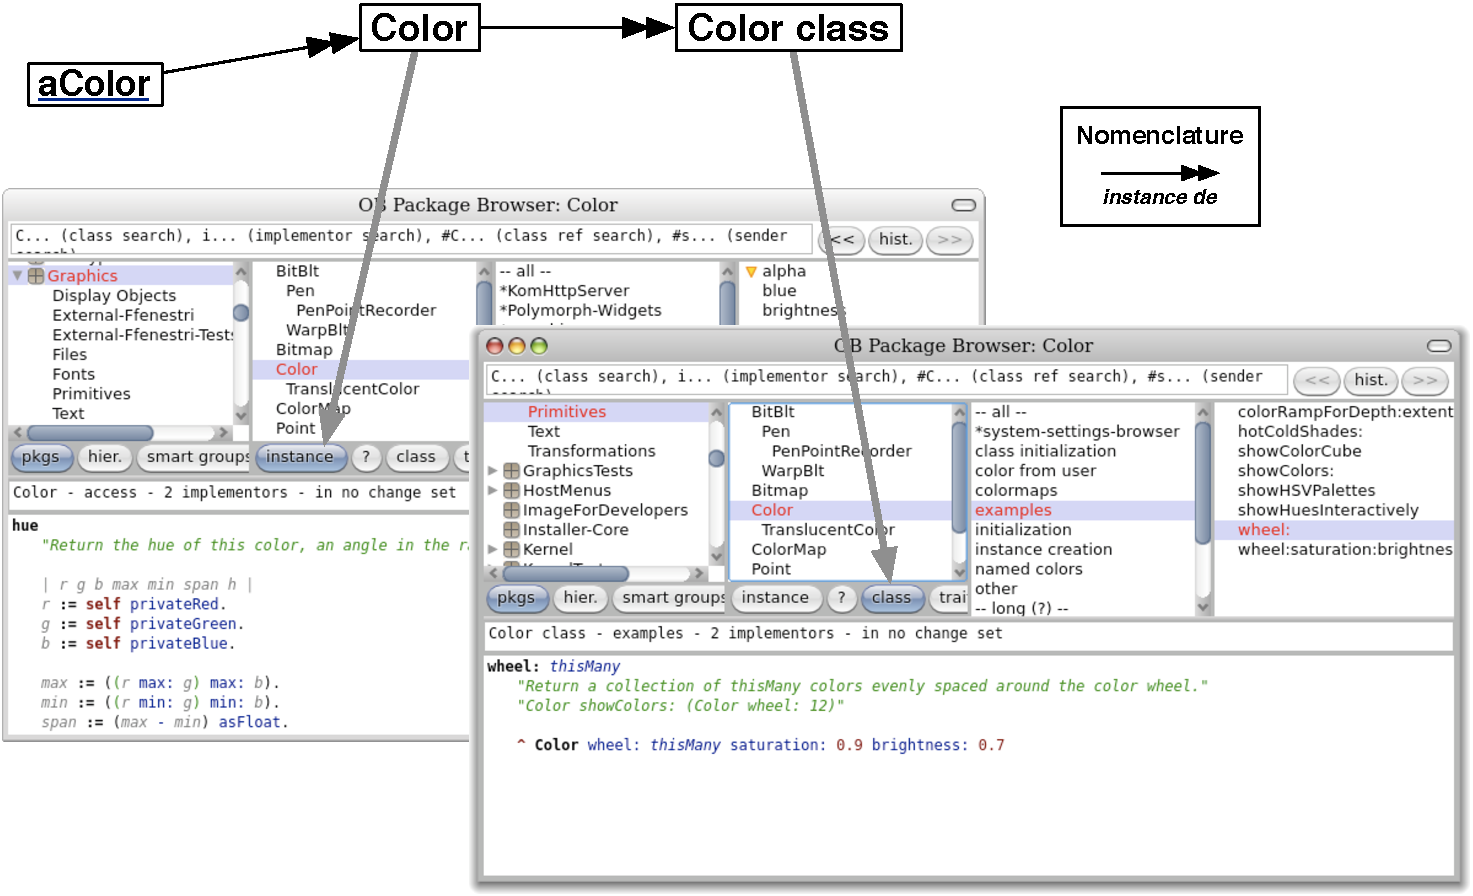
\includegraphics[width=\textwidth]{Color-Buttons}
\caption{Naviguer dans une classe et sa méta-classe.
% \sd{Do we use Key everywhere in the picture as a legend indicator?}
% \on{sure, wherever appropriate}
\figlabel{Buttons}}
\end{center}
\end{figure}

De ce fait, le navigateur de classes nommé \ind{Browser} vous
aide à parcourir à la fois classes et méta-classes comme si elles
n'étaient qu'une seule entité avec deux ``côtés'': le ``\subind{Browser}{côté instance}'' et le ``\subind{Browser}{côté classe}'', comme le montre \figref{Buttons}. 
\damien{something wrong here. The text between quotes is not generated}
% true: \ind should replace \index there! (martial)
En \clickant{} sur le bouton \button{instance}, vous voyez la présentation de la classe \ct{Color} et vous donc pouvez naviguer dans les méthodes qui sont exécutées quand les messages de même nom sont envoyés à une instance de \ct{Color}, comme par exemple \lct{blue} (correspondant à la couleur bleu). En appuyant
sur le bouton \button{class} (pour classe), vous naviguez dans la classe \ct{Color class}, autrement dit vous voyez les méthodes qui seront exécutées en envoyant les messages directement à la classe \ct{Color} elle-même.
Par exemple, \ct{Color blue} envoie le message \ct{blue} (pour \emph{bleu}) à la classe \clsind{Color}.
Vous trouverez donc la méthode \ct{blue} définie côté classe de la classe \ct{Color} et non du côté instance.
\seeindex{côté instance}{Browser!côté instance}
\seeindex{côté classe}{Browser!côté classe}
\seeindex{navigateur de classes!côté instance}{Browser!côté instance}
\seeindex{navigateur de classes!côté classe}{Browser!côté classe}


\needlines{5}
\begin{code}{@TEST | aColor |}
aColor := Color blue.               "!Méthode! de classe blue"
aColor        --> Color blue
aColor red  --> 0.0         "!Méthode d'accès red (rouge) côté instance!"
aColor blue --> 1.0        "!Méthode d'accès blue (bleu) côté instance!"
\end{code}

Vous définissez une classe en remplissant le patron (ou \emph{template} en anglais) proposé
dans le \subind{Browser}{côté instance}.
Quand vous acceptez ce patron, le système crée non seulement la classe
que vous définissez mais aussi la méta-classe correspondante.
Vous pouvez naviguer dans la méta-classe en \clickant{} sur le bouton \button{class}.
Du patron employé pour la création de la méta-classe, seule la
liste des noms des variables d'instance vous est proposée pour une édition directe.  

Une fois que vous avez créé une classe, \click{} sur
le bouton \button{instance} vous permet d'éditer et de parcourir les
méthodes qui seront possédées par les instances de cette classe (et de ses sous-classes). Par exemple, nous pouvons voir dans \figref{Buttons} que 
la méthode \ct{hue} est définie pour les instances de la classe \ct{Color}.
A contrario, le bouton \button{class} vous laisse parcourir et éditer
la méta-classe (dans ce cas \ct{Color class}).

%---------------------------------------------------------
\subsection{Les méthodes de classe} 

Les méthodes de classe peuvent être relativement utiles; naviguez dans \ct{Color class} pour voir quelques bons exemples.
Vous verrez qu'il y a deux sortes de \subind{classe}{méthode}{s} définies dans une classe: celles qui créent les instances de la classe, comme \cmind{Color class}{blue} et celles qui ont une action \emph{utilitaire}, 
% martial: j'ai mis volontairement \emph pour l'adjectif utilitaire
comme \cmind{Color class}{showColorCube}.
Ceci est courant, bien que vous trouverez occasionnellement des méthodes de classe utilisées d'une autre manière.

Il est commun de placer des méthodes utilitaires dans le \subind{Browser}{côté classe} parce qu'elles peuvent être exécutées
sans avoir à créer un objet additionnel dans un premier temps. 
% coutumier -> commun
En fait, beaucoup d'entre elles contiennent un commentaire pour les rendre plus compréhensibles pour l'utilisateur qui les exécute.

\dothis{Naviguez dans la méthode \ct{Color class>>>showColorCube}, double-cliquez à l'intérieur des guillemets englobant le commentaire \ct{"Color showColorCube"} et tape au clavier \short{d}.}
Vous verrez l'effet de l'exécution de cette méthode.  (Sélectionnez \menu{World \go \ind{restore display}~(r)} pour annuler les effets.)

Pour les familiers de \ind{Java} et \ind{C++},  les méthodes de classe peuvent être assimilées aux méthodes statiques. 
Néanmoins, l'homogénéité de \st induit une différence:  les méthodes statiques de Java sont des fonctions résolues de manière statique alors que les méthodes de classe de \st sont des méthodes à transfert dynamique~\footnote{En anglais, dynamically-dispatched methods.} Ainsi, l'héritage, la surcharge et l'utilisation de \emph{super} fonctionnent avec les méthodes de classe dans \st, ce qui n'est pas le cas avec les méthodes statiques en Java.  

%---------------------------------------------------------
\subsection{Les variables d'instance de classe}
Dans le cadre des variables d'instance ordinaires, toutes les instances d'une classe partagent le même ensemble
de noms de variable et les instances de ses sous-classes héritent de ces noms; cependant, chaque instance possède son propre jeu de valeurs.
C'est exactement la même histoire avec les \subind{classe!variables d'instance}{variables d'instance de classe}: chaque classe a ses propres variables d'instance de classe privées.
Une sous-classe héritera de ces  variables d'instance de classe, \emph{mais elle aura ses propres copies privées de ces variables}.
Aussi vrai que les objets ne partagent pas les variables d'instance, les classes et leurs sous-classes ne partagent pas les variables d'instance de classe.

Vous pouvez utiliser une variable d'instance de classe \ct{count}~\footnote{En français, compteur.} afin de suivre le nombre d'instances que vous créez pour une classe donnée.
Cependant, les sous-classes ont leur propre variable \ct{count}, 
les instances des sous-classes seront comptées séparément.

\paragraph{Exemple: les variables d'instance de classe ne sont pas partagées avec les sous-classes.}
Soient les classes \ct{Dog} et \ct{Hyena}~\footnote{En français, chien et hyène.} telles que \ct{Hyena} hérite de la variable d'instance de classe \ct{count} de la classe \ct{Dog}.

%martial: si mauvaise coupe:
%\newpage
\begin{classdef}[dog]{Créer Dog et Hyena}
Object subclass: #Dog
	instanceVariableNames: ''
	classVariableNames: ''
	poolDictionaries: ''
	category: 'PBE-CIV'

Dog class
	instanceVariableNames: 'count'

Dog subclass: #Hyena
	instanceVariableNames: ''
	classVariableNames: ''
	poolDictionaries: ''
	category: 'PBE-CIV'
\end{classdef}

Supposons que nous ayons des méthodes de classe de \ct{Dog} pour initialiser sa variable \ct{count} à \ct{0} et pour incrémenter cette dernière quand de nouvelles instances sont créées:
\begin{method}[dogcount]{Comptabiliser les nouvelles instances de \ct{Dog} via \ct{Dog class>>>count}}
Dog class>>>initialize
	super initialize.
	count := 0.

Dog class>>>new
	count := count +1.
	^ super new

Dog class>>>count
	^ count
\end{method}

Maintenant, à chaque fois que nous créons un nouveau \ct{Dog}, son compteur
count est incrémenté. Il en est de même pour toute nouvelle instance de \ct{Hyena}, mais elles sont comptées séparément:
\begin{code}{}
Dog initialize.
Hyena initialize.
Dog count     --> 0
Hyena count --> 0
Dog new.
Dog count     --> 1
Dog new.
Dog count     --> 2
Hyena new.
Hyena count --> 1
\end{code}
% ON: In order to make this a test, I need the previous code to be part of the setup. Bleh.

Remarquons aussi que les variables d'instance de classe sont privées à la classe tout comme les variables d'instance sont privées à l'instance. 
Comme les classes et leurs instances sont des objets différents,
il en résulte que:
\important{Une classe n'a pas accès aux variables d'instance de ses propres instances.}
\important{Une instance d'une classe n'a pas accès aux variables d'instance de classe de sa classe.}
C'est pour cette raison que les méthodes d'initialisation d'instance doivent 
toujours être définies dans le \subind{Browser}{côté instance}\,---\,le \subind{Browser}{côté classe} n'ayant pas accès aux variables d'instance, il ne pourrait y avoir initiali\-sation!  
% 2007-11-05 correction errata SBE
Tout ce que peut faire la classe, c'est d'envoyer des messages d'\ind{initialisation} à des instances nouvellement créées; ces messages pouvant bien sûr utiliser les méthodes d'\subind{méthode}{accès}.

De même, les instances ne peuvent accéder aux variables d'instance de classe
que de manière indirecte en envoyant les messages d'accès à leur classe.

\ind{Java} n'a rien d'équivalent aux variables d'instance de classe.  
Les variables statiques en Java et en \ind{C++} ont plutôt des similitudes 
avec les variables de classe de \st dont nous parlerons dans \secref{classVars}: toutes les sous-classes et leurs instances partagent la même variable statique.

\paragraph{Exemple: Définir un Singleton.}
Le patron de conception~\footnote{En anglais, nous parlons de \emph{Design Patterns}.} nommé \ind{Singleton}~\cite{Alpe98a} offre un exemple-type de l'usage de variables d'instance de classe et de méthodes de classe.
Imaginez que nous souhaitions d'une part, créer une classe \ct{WebServer} et d'autre part, s'assurer qu'il n'a qu'une et une seule instance en faisant appel au patron Singleton.

En \clickant{} sur le bouton \button{instance} dans le navigateur de classe, nous définissons la classe \clsind{WebServer} comme suit (\clsref{singleton}).

\begin{classdef}[singleton]{Une classe Singleton}
Object subclass: #WebServer
	instanceVariableNames: 'sessions' 	
	classVariableNames: '' 	
	poolDictionaries: ''
	category: 'Web'
\end{classdef}

Ensuite, en \clickant{} sur le bouton \button{class}, nous pouvons ajouter une variable d'instance \ct{uniqueInstance} au \subind{Browser}{côté classe}.

\begin{classdef}[webserver]{Le côté classe de la classe Singleton}
WebServer class 	
	instanceVariableNames: 'uniqueInstance'
\end{classdef}

Par conséquence, la classe \ct{WebServer} a désormais une autre variable d'instance, en plus des variables héritées telles que \ct{superclass} et \ct{methodDict}.

Nous pouvons maintenant définir une \subind{classe}{méthode} de classe que nous appellerons \ct{uniqueInstance} comme dans \tmthref{uniqueInstance}. 
Pour commencer, cette méthode vérifie si \ct{uniqueInstance} a été initialisée ou non: dans ce dernier cas,
la méthode crée une instance et l'assigne à la variable d'instance de classe \ct{uniqueInstance}.  
\emph{In fine}, la valeur de \ct{uniqueInstance} est retournée.
Puisque \ct{uniqueInstance} est une variable d'instance de classe, cette méthode peut directement y accéder.

\needlines{4}
\begin{method}[uniqueInstance]{\ct{WebServer class>>>uniqueInstance} (côté classe)}
WebServer class>>>uniqueInstance
     uniqueInstance ifNil: [uniqueInstance := self new].
     ^ uniqueInstance
\end{method}

La première fois que l'expression \ct{WebServer uniqueInstance} est exécutée, une instance de la classe \ct{WebServer} sera créée et affectée à la variable \ct{uniqueInstance}. 
La seconde fois, l'instance précédemment créée sera retournée au lieu d'y avoir une nouvelle création. 

Remarquons que la clause conditionnelle à l'intérieur du code de création
de \tmthref{uniqueInstance} est écrite \ct{self new} et non 
\mbox{\ct{WebServer new}.}
Quelle en est la différence?   Comme la méthode \ct{uniqueInstance} est définie dans \mbox{\ct{WebServer class},} vous pouvez penser qu'elles sont identiques.    En fait, tant que personne ne crée une sous-classe de \ct{WebServer}, elles sont pareilles. Mais en supposant que \ct{ReliableWebServer} est une sous-classe de \ct{WebServer} et qu'elle hérite de la méthode \ct{uniqueInstance},
nous devrions nous attendre à ce que \ct{ReliableWebServer uniqueInstance} réponde un \ct{ReliableWebServer}. L'utilisation de \self assure que cela arrivera car il sera lié à la classe correspondante.
Du reste, notez que \ct{WebServer} et \ct{ReliableWebServer} ont chacune
leur propre variable d'instance de classe nommée \ct{uniqueInstance}.  

% proposition de Rene :
% Ces deux variables ont, bien entendu, différentes valeurs.
Ces deux variables ont, bien entendu, différentes valeurs.

%=========================================================
\section{Toute classe a une super-classe}

%\ruleref{inheritance}

Chaque classe en \st hérite de son comportement et de la description
de sa structure d'une unique \emphind{super-classe}.
Ceci est équivalent à dire que \st a un \ind{héritage} simple.

\needlines{2}
\begin{code}{@TEST}
SmallInteger superclass --> Integer
Integer superclass          --> Number
Number superclass        --> Magnitude
Magnitude superclass    --> Object
Object superclass           --> ProtoObject
ProtoObject superclass  --> nil
\end{code}

Traditionnellement, la racine de la hiérarchie d'héritage en \st est la classe \clsind{Object} (``Objet'' en anglais; puisque \mantra).
En \pharo, la racine est en fait une classe nommée \clsind{ProtoObject}, mais
normalement, vous n'aurez aucune attention à accorder à cette classe.
\ct{ProtoObject} encapsule le jeu de messages restreint que tout objet \emph{doit} avoir.  
N'importe comment, la plupart des classes héritent de \ct{Object} qui, pour
sa part, définit beaucoup de messages supplémentaires que presque tous les
objets devraient comprendre et auquels ils devraient pouvoir répondre.
à moins que vous ayez une autre raison de faire autrement, vous devriez
normalement générer des classes d'application par l'héritage
de la classe \ct{Object} ou d'une de ses sous-classes lors de la création de classe.

\dothis{Une nouvelle classe est normalement créée par l'envoi du message
\ct{subclass: instanceVariableNames: ...}
à une classe existante.
Il y a d'autres méthodes pour créer des classes.
Veuillez jeter un coup d'\oe il au protocole \prot{Kernel-Classes \go Class \go subclass creation} pour voir desquelles il s'agit.}
\scatindex{Kernel-Classes}
\protindex{création}

%There is no special syntax for creating abstract classes in \st.
%An abstract class is an ordinary class in which the implementation of some methods is deferred to a subclass.
%This is repeated in the next section

Bien que \pharo ne dispose pas d'héritage multiple, il dispose d'un mécanisme appelé % CHANGE 
% martial: footnote ajoute
\emphind{trait}{}s~\footnote{Dans le sens de trait de caractères, nous faisons allusion ainsi à la génétique du comportement d'une méthode.} 
pour partager le comportement entre des classes distincts.
Les \emph{traits} sont des collections de méthodes qui peuvent être réutilisées par plusieurs classes sans lien d'héritage. Employer les \emph{traits} vous permet de partager du code entre les différentes classes sans reproduire ce code.

%---------------------------------------------------------
\subsection{Les méthodes abstraites et les classes abstraites}

Une classe \subind{classe}{abstraite} est une classe qui n'existe que pour être héritée, au lieu d'être instanciée.
Une classe abstraite est habituellement incomplète, dans le sens qu'elle ne définit pas toutes les méthodes qu'elle utilise.
Les méthodes ``manquantes''\,---\,celle que les autres méthodes envoyent, mais qui ne sont pas définies elles-mêmes\,---\,sont dites mé\-tho\-des \subind{méthode}{abstraite}{s}.
\seeindex{classe abstraite}{classe, abstraite}
\seeindex{méthode abstraite}{méthode, abstraite}

\st n'a pas de syntaxe dédiée pour dire qu'une méthode ou qu'une classe est abstraite. 
Par convention, le corps d'une méthode abstraite contient l'expression \ct{self subclassResponsibility}~\footnote{Dans le sens, laissée à la responsabilité de la sous-classe.}. 
Ceci est connu sous le nom de ``marker method'' ou marqueur de méthode; il indique que les sous-classes ont la responsabilité de définir une version concrète de la méthode. 
Les méthodes \ct{self subclassResponsibility} devraient toujours être surchargées, et ainsi, ne devraient jamais être exécutées.
Si vous oubliez d'en surcharger une et que celle-ci est exécutée, une exception sera levée. 
\cmindex{Object}{subclassResponsibility}

Une classe est considérée comme abstraite si une de ses méthodes est abstraite.
Rien ne vous empêche de créer une instance d'une classe abstraite; tout fonctionnera jusqu'à ce qu'une méthode abstraite soit invoquée. 

\subsubsection{Exemple: la classe \ct{Magnitude}.}
\clsind{Magnitude} est une classe abstraite qui nous aide à définir
des objets pouvant être comparables les uns avec les autres. Les
sous-classes de \ct{Magnitude} devraient implémenter les méthodes
\ct{<}, \ct{=} et \ct{hash}~\footnote{Relatif au code de hachage.}.
Grâce à ces messages, \ct{Magnitude} définit d'autres méthodes telles que
\mbox{\ct{>},} \mbox{\ct{>=},} \mbox{\ct{<=},} \mbox{\ct{max:},} \mbox{\ct{min:},} \ct{between:and:} et
d'autres encore pour comparer des objets.
Ces méthodes sont héritées par les sous-classes.
La méthode \mthind{Magnitude}{<} est abstraite et est définie comme
dans \tmthref{MagnitudeLessThan}.

\begin{method}[MagnitudeLessThan]{\ct{Magnitude>>><}. Le commentaire dit: ``répond si le receveur est inférieur à l'argument''}
Magnitude>>>< aMagnitude 
	"Answer whether the receiver is less than the argument."
	^ self subclassResponsibility
\end{method}

\noindent
A contrario, la méthode \mthind{Magnitude}{>=} est concrète; elle est définie en fonction de \ct{<}:

\begin{method}[Magnitude>=]{\ct{Magnitude>>>>=}. Le commentaire dit: ``répond si le receveur est plus grand ou égal à l'argument''}
>= aMagnitude 
	"Answer whether the receiver is greater than or equal to the argument."
	^ (self < aMagnitude) not
\end{method}
Il en va de même des autres méthodes de comparaison.

\clsind{Character} est une sous-classe de \ct{Magnitude}; elle surcharge la méthode \mthind{Object}{subclassResponsibility} de \ct{<} avec sa propre version de \ct{<} (voir \mthref{CharacterLessThan}).  \ct{Character} définit aussi les méthodes \ct{=} et \ct{hash}; elles héritent entre autre des méthodes \mbox{\ct{>=},} \ct{<=} et \ct{~=} de la classe \ct{Magnitude}.

\begin{method}[CharacterLessThan]{\ct{Character>>><}. Le commentaire dit: ``répond vrai si la valeur du receveur est inférieure à la valeur du l'argument''}
Character>>>< aCharacter 
	"Answer true if the receiver's value < aCharacter's value."
	^ self asciiValue < aCharacter asciiValue
\end{method}

%---------------------------------------------------------
\subsection{Traits}
Un \emphind{trait} est une collection de méthodes qui peut être incluse dans le comportement d'une classe sans le besoin d'un héritage.
Les classes disposent non seulement d'une seule super-classe mais aussi de la facilité offerte par le partage de méthodes utiles avec d'autres méthodes sans lien de parenté vis-à-vis de l'héritage.

Définir un nouveau \emph{trait} se fait en remplaçant simplement le patron
pour la création de la sous-classe par un message à la classe \clsind{Trait}.

\needspace{5\baselineskip}
\begin{classdef}[tauthor]{Définir un nouveau \emph{trait}}
Trait named: #TAuthor
	uses: { }
	category: 'PBE-LightsOut'
\end{classdef}

\noindent
Nous définissons ici le \emph{trait} \ct{TAuthor} dans la catégorie \scat{PBE-LightsOut}.
Ce \emph{trait} n'\emph{utilise}~\footnote{Terme anglais: \emph{uses}: il signifie ``utilise''.} aucun autre \emph{trait} existant.
En général, nous pouvons spécifier l'\emph{expression de composition d'un trait} par d'autres \emph{traits} en u\-ti\-li\-sant le mot-clé \ct{uses:}.
Dans notre cas, nous écrivons un tableau vide \mbox{(\{ \}).}

Les \emph{traits} peuvent contenir des méthodes, mais aucune variable d'instance.
Supposons que nous voulons ajouter une méthode \ct{author} (auteur en anglais) à différentes classes sans lien hiérarchique;
nous le ferions ainsi:

\begin{method}[author]{Définir la méthode \ct{TAuthor>>>author}}
TAuthor>>>author
    "Returns author initials"
	^ 'on'    "oscar nierstrasz"
\end{method}

\noindent
Maintenant nous pouvons employer ce \emph{trait} dans une classe ayant déjà sa propre super-classe, disons, la classe \ct{LOGame} que nous avons définie dans \charef{firstApp}.
Nous n'avons qu'à modifier le patron de création de la classe \ct{LOGame} pour y inclure cette fois l'argument-clé \ct{uses:} suivi du \emph{trait} à utiliser: \ct{TAuthor}.

\begin{classdef}[sbegamewithtrait]{Utiliser un trait}
BorderedMorph subclass: #LOGame
	uses: TAuthor
	instanceVariableNames: 'cells'
	classVariableNames: ''
	poolDictionaries: ''
	category: 'PBE-LightsOut'
\end{classdef}

Si nous instançions maintenant \ct{LOGame}, l'instance répondra comme prévu au message \ct{author}.

\begin{code}{}
LOGame new author --> 'on'
\end{code}

Les expressions de composition de \emph{trait} peuvent combiner plusieurs \emph{traits} via l'opérateur \ct{+}.
En cas de conflit (\ie quand plusieurs \emph{traits} définissent des méthodes avec le même nom), ces conflits peuvent être résolus en retirant explicitement ces méthodes (avec \ct{-}) ou en redéfinissant ces méthodes dans la classe ou le \emph{trait} que vous êtes en train de définir.
Il est possible aussi de créer un \emph{alias} des méthodes (avec \ct{@}) 
leur fournissant ainsi un nouveau nom.

Les \emph{traits} sont employés dans le noyau du système~\footnote{En anglais, System kernel.}.
Un bon exemple est la classe \mbox{\clsind{Behavior}.}

\needlines{8}
\begin{classdef}[behaviorwithtraits]{Behavior définit par les \emph{traits}}
Object subclass: #Behavior
	uses: TPureBehavior @ {#basicAddTraitSelector:withMethod:->#addTraitSelector:withMethod:}
	instanceVariableNames: 'superclass methodDict format'
	classVariableNames: 'ObsoleteSubclasses'
	poolDictionaries: ''
	category: 'Kernel-Classes'
\end{classdef}
\noindent
Ici, nous voyons que la méthode \ct{basicAddTraitSelector:withMethod:} définie dans le \emph{trait} \ct{TPureBehavior} a été renommée en \mbox{\ct{addTraitSelector:withMethod:}.}
%-Here we see that the method \ct{addTraitSelector:withMethod:} defined in the trait \ct{TPureBehavior} has been aliased to \ct{basicAddTraitSelector:withMethod:}.
Les \emph{traits} sont à présent supportés par les navigateurs de classe (ou \emph{browsers}).

%=========================================================
\section{Tout se passe par envoi de messages} % REVOIR 'by sending messages'

%\ruleref{message}

Cette règle résume l'essence même de la programmation en \st.

Dans la programmation procédurale, lorsqu'une procédure est appelée, l'appelant (\emph{caller}, en anglais) fait le choix du morceau de code à exécuter; il choisit la procédure ou la fonction à exécuter \emph{statiquement}, par nom.  

En programmation orientée objet, nous ne faisons \emph{pas}
d'``appel de méthodes''. Nous faisons un ``\subind{message}{envoi}
de messages.'' % REVOIR 'by sending messages'
Le choix de terminologie est important.
Chaque objet a ses propres responsabilités.
Nous ne pouvons \emph{dire} à un objet ce qu'il faut faire en lui imposant 
une procédure.
Au lieu de cela, nous devons lui \emph{demander} poliment de faire quelque chose en lui envoyant un message.
Le message n'est \emph{pas} un morceau de code: ce n'est rien d'autre qu'un nom (sélecteur) et une liste d'arguments.
Le receveur décide alors de comment y répondre en sélectionnant en retour
sa propre méthode correspondant à ce qui a été demandé.
Puisque des objets distincts peuvent avoir différentes méthodes pour répondre à un même message, le choix de la méthode doit se faire \emph{dynamiquement} à la réception du message.
\begin{code}{@TEST}
3 + 4         --> 7          "!envoie le message + d'argument 4 à l'entier  3!"
(1@2) + 4 --> 5@6    "envoie le message + d'argument 4 au point (1@2)"
\end{code}
\noindent
En conséquence, nous pouvons envoyer le \emph{même message} à différents objets, chacun pouvant avoir \emph{sa propre méthode} en réponse au message.
Nous ne disons pas à \ct{SmallInteger} \ct{3} ou au \ct{Point} \ct{1@2} comment répondre au message \ct{+ 4}.
Chacun a sa propre méthode pour répondre à cet envoi de message, et répond ainsi selon le cas.

L'une des conséquences du modèle d'envoi de messages de \st est
qu'il encourage un style de programmation dans lequel les objets
tendent à avoir des méthodes très compactes en déléguant des
tâches aux autres objets, plutôt que d'implémenter de
gigantesques méthodes procédurales engendrant trop de
responsabilité. % REVOIR 'by sending messages'
Joseph Pelrine
\ab{Citation?}
\on{désolé, simple communiqué personel de l'auteur et notes de lecture!}
dit succintement le principe suivant:
\important{Ne fais rien que tu ne peux déléguer à quelqu'un d'autre~\traduit{Don't do anything that you can push off onto someone else.}.}
\index{Pelrine, Joseph}

Beaucoup de langages orientés objets disposent à la fois
d'opérations statiques et dynamiques pour les objets; en \st il n'y
a qu'envois de messages dynamiques. Au lieu de fournir des
opérations statiques sur les classes, nous leur envoyons simplement
des messages, puisque les classes sont aussi des objets. % REVOIR 'by sending messages'

\emph{Pratiquement} tout en \st se passe par envoi de messages. % REVOIR 'by sending messages'
à certains stades, le pragmatisme doit prendre le relais:
\begin{itemize}
  \item Les \emph{déclarations de variable} ne reposent pas sur l'envoi de messages.
  		En fait, les \subind{variable}{déclaration}{}s de variable ne sont même pas exécutables.
  		Déclarer une variable produit simplement l'allocation d'un espace pour la référence de l'objet.
  \item Les \emph{affectations} (ou assignations) ne reposent pas sur l'envoi de messages.
  		L'\ind{affectation} d'une variable produit une liaison de nom de variable dans le cadre de sa définition.
  \item Les \emph{retours} (ou renvois) ne reposent pas sur l'envoi de message.
  		Un \ind{retour} ne produit que le retour à l'envoyeur du résultat calculé.
  \item Les \emph{primitives} ne reposent pas sur l'envoi de message.
  		Elles sont codées au niveau de la \ind{machine virtuelle}.
		\index{primitive}
\end{itemize}

à quelques autres exceptions près, presque tout le reste se déroule véritablement par l'envoi de messages. 
En particulier, la seule façon de mettre à jour une \ind{variable d'instance} d'un autre objet est de lui envoyer un message réclamant le changement de son propre attribut (ou champ) car ces derniers ne sont pas des ``attributs publics'' en \st.
Bien entendu, offrir des méthodes d'\subind{méthode}{accès en lecture} dites accesseurs (\emph{getter}, en anglais, retournant l'état de la variable) et mutateurs ou méthodes d'\subind{méthode}{accès en écriture} (\emph{setter} en anglais, changeant la variable) pour chaque variable d'instance d'un objet n'est pas une bonne méthodologie orientée objet.
Joseph Pelrine annonce aussi à juste titre:
\important{Ne laissez jamais personne d'autre jouer avec vos données~\traduit{Don't let anyone else play with your data.}.}

%=========================================================
\section{La recherche de méthode suit la chaîne d'héritage} 

%\ruleref{lookup}

Qu'arrive-t-il exactement quand un objet reçoit un message?

Le processus est relativement simple:
la classe du receveur cherche la méthode à utiliser pour opérer le message.
Si cette classe n'a pas de méthode, elle demande à sa \ind{super-classe} et remonte ainsi de suite la chaîne d'\ind{héritage}.
Quand la méthode est enfin trouvée, les arguments sont affectés aux paramètres de la méthode et la \ind{machine virtuelle} l'exécute.
\index{méthode!lookup}
\index{méthode!réferencement}

C'est, en essence, aussi simple que cela.
Mais il reste quelques questions auxquelles nous devons prendre soin de répondre:

\begin{itemize}
  \item \emph{Que se passe-t-il lorsque une méthode ne renvoie pas explicitement une valeur?}
  \item \emph{Que se passe-t-il quand une classe réimplémente une méthode d'une super-classe?}
  \item \emph{Quelle différence y a-t-il entre les envois faits à \pvind{self} et ceux faits à \pvind{super}?}
  \item \emph{Que se passe-t-il lorsqu'aucune méthode est trouvée?}
\end{itemize}

Les règles pour la recherche par référencement (en anglais \emph{lookup}) présentées ici sont conceptuelles: des réalisations au sein de la machine virtuelle rusent pour optimiser la vitesse de recherche des méthodes. 
C'est leur travail mais tout est fait pour que vous ne remarquiez jamais qu'elles font quelque chose de différent des règles énoncées.
% Whatever the implementation does, these rules will give you a clear understanding of the semantics of sending messages to \self and \super.

Tout d'abord, penchons-nous sur la stratégie de base de la recherche. Ensuite nous répondrons aux questions.

%---------------------------------------------------------
\subsection{La recherche de méthode}
Supposons la création d'une instance de \ct{EllipseMorph}.
\begin{code}{@TEST | anEllipse |}
anEllipse := EllipseMorph new.
\end{code}
\noindent
Si nous envoyons à cet objet le message \ct{defaultColor}, nous obtenons le résultat \ct{Color yellow}~\footnote{Yellow est la couleur jaune.}:
\begin{code}{@TEST | anEllipse | anEllipse := EllipseMorph new.}
anEllipse defaultColor --> Color yellow
\end{code}
\noindent
La classe \ct{EllipseMorph} implémente \ct{defaultColor}, donc la méthode adéquate est trouvée immédiatement.

\needlines{5}
\begin{method}[defaultColor]{Une méthode implémentée localement. Le commentaire dit: ``retourne la couleur par défaut; le style de remplissage pour le receveur''}
EllipseMorph>>>defaultColor
	"answer the default color/fill style for the receiver"
	^ Color yellow
\end{method}
\cmindex{EllipseMorph}{defaultColor}

A contrario, si nous envoyons le message \ct{openInWorld} à \mbox{\ct{anEllipse},} la méthode n'est pas trouvée immédiatement parce que la classe \ct{EllipseMorph} n'implémente pas \ct{openInWorld}.
La recherche continue plus avant dans la super-classe \mbox{\ct{BorderedMorph},} puis ainsi de suite, jusqu'à ce qu'une méthode \ct{openInWorld} soit trouvée dans la classe \ct{Morph} (voir \figref{openInWorldLookup}).

\begin{method}[openInWorld]{Une méthode héritée. Le commentaire dit: ``Ajoute ce morph dans le monde (world).''}
Morph>>>openInWorld
	"Add this morph to the world."

  self openInWorld: self currentWorld
\end{method}
\cmindex{Morph}{openInWorld}

\begin{figure}[htb]
\begin{center}
	{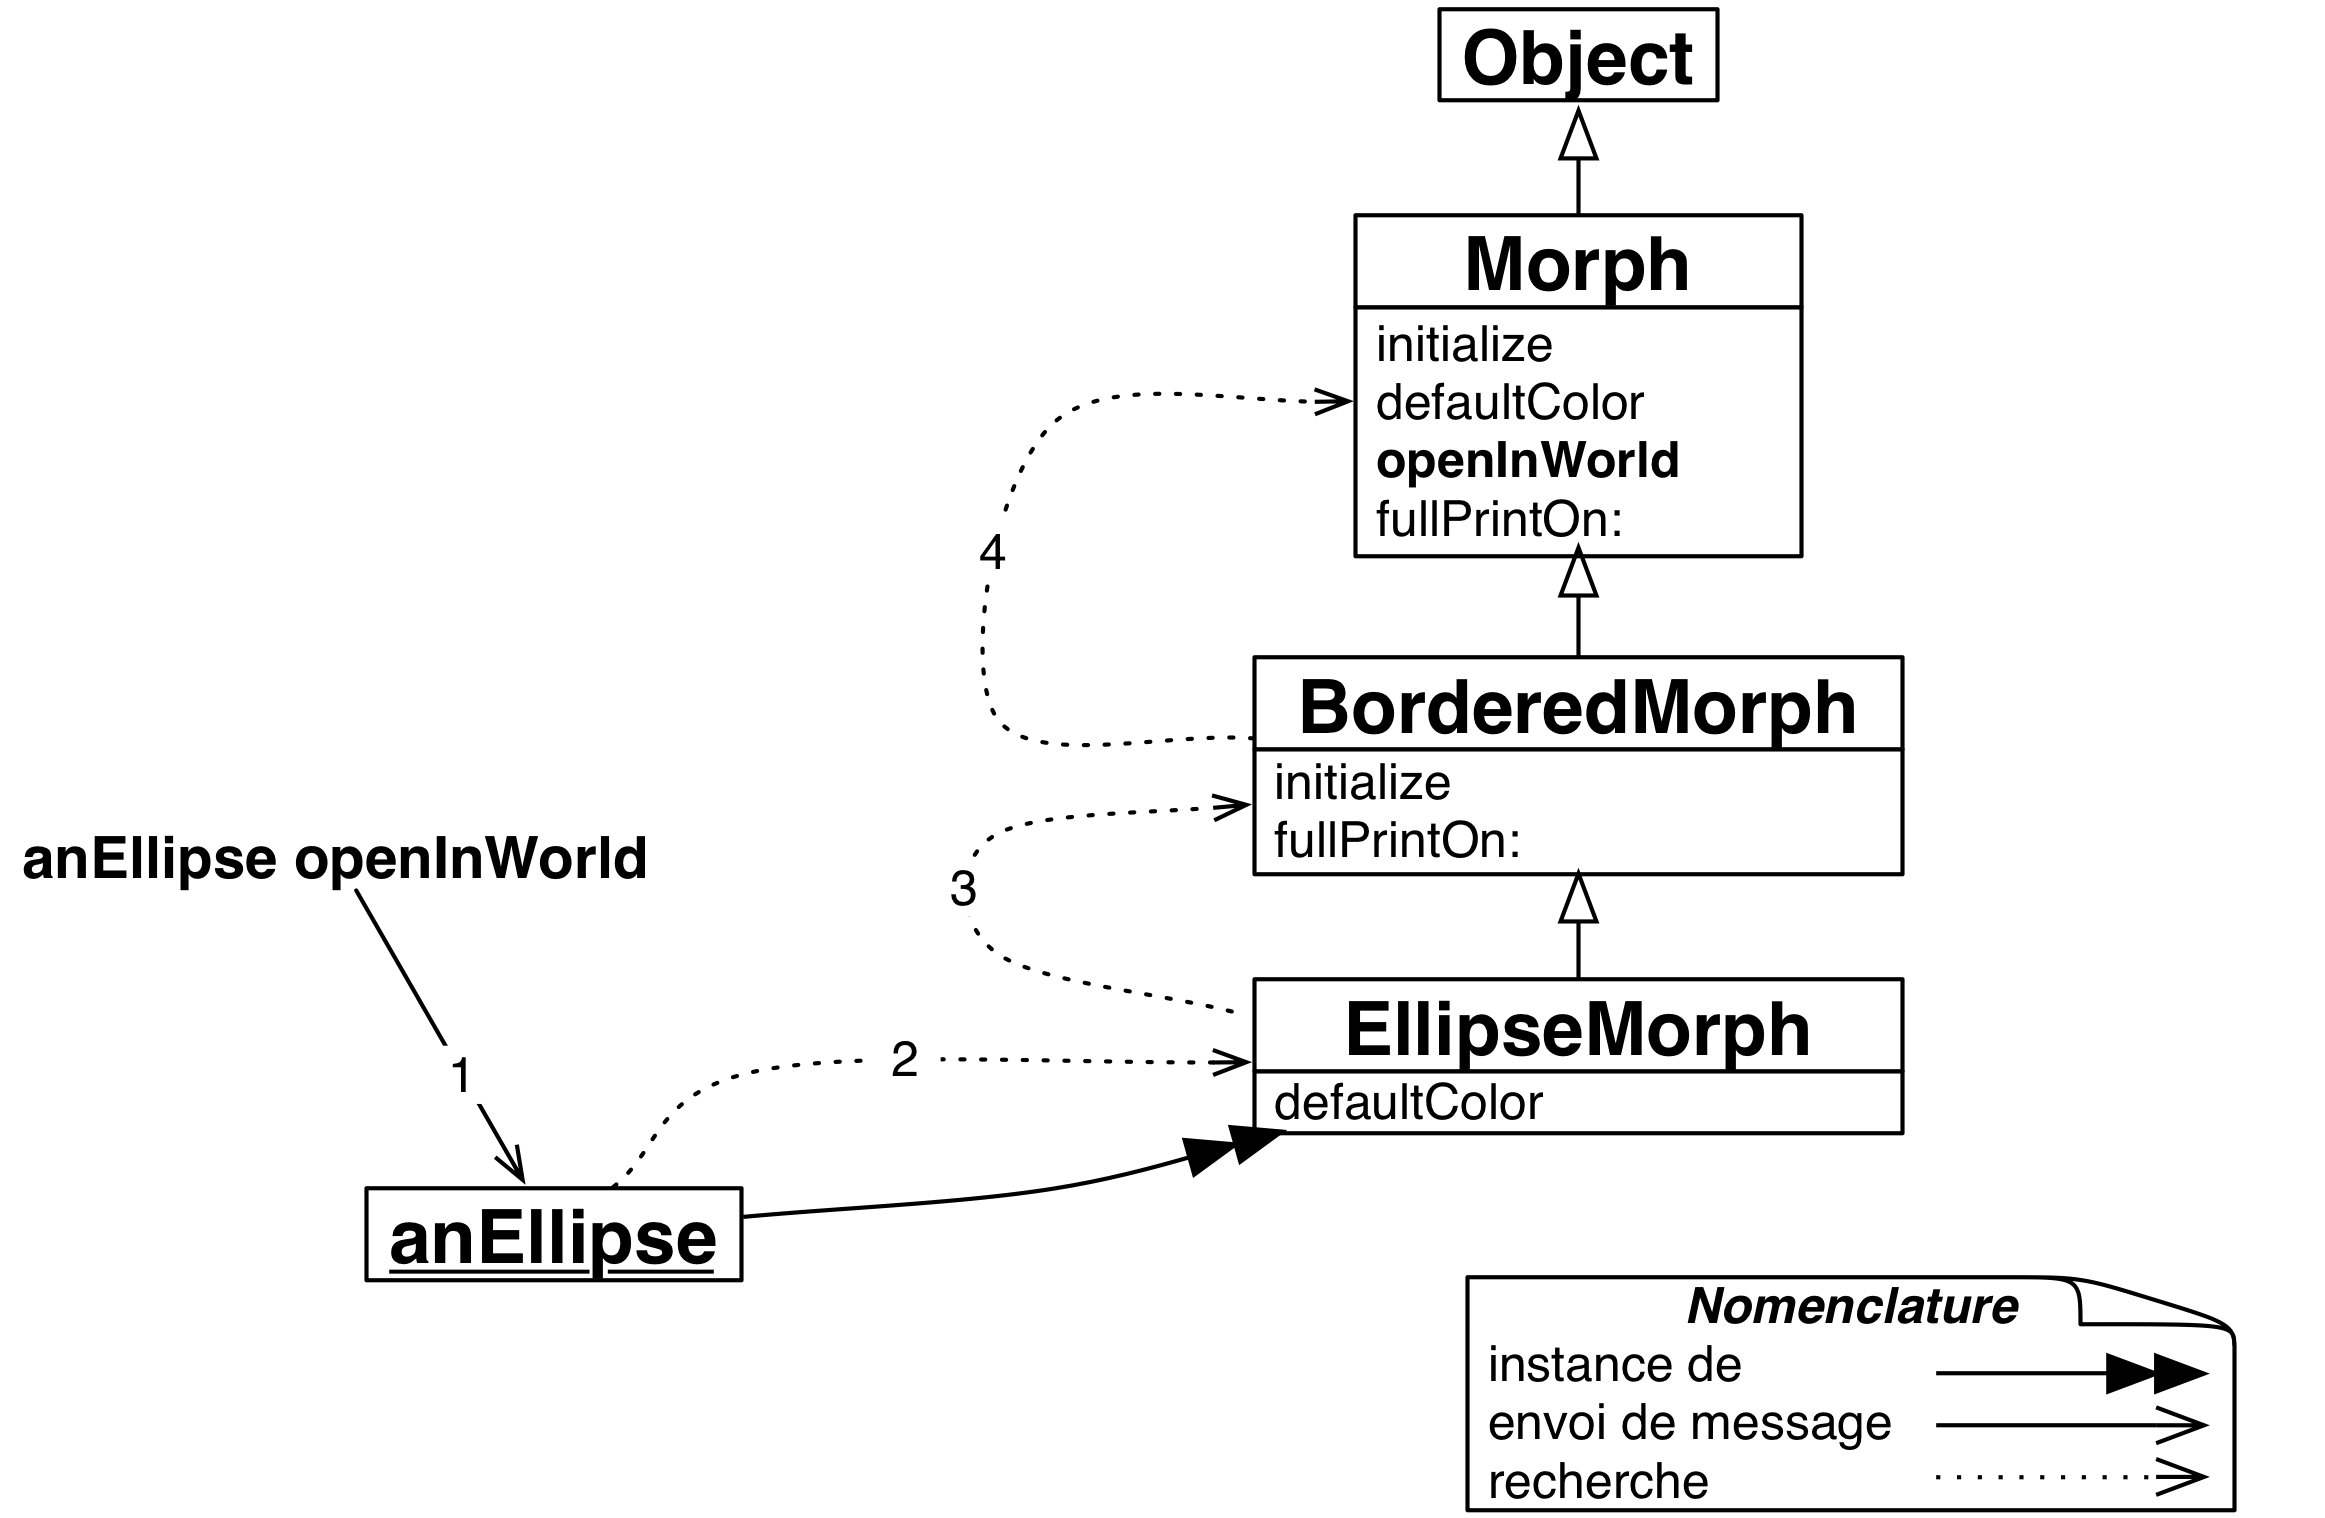
\includegraphics[width=0.8\textwidth]{openInWorldLookup}}
\caption{Recherche par référencement d'une méthode suivant la hiérarchie d'héritage.\figlabel{openInWorldLookup}}
\end{center}
\end{figure}

%---------------------------------------------------------
\subsection{Renvoyer self}

Remarquez que \ct{EllipseMorph>>>defaultColor} (\mthref{defaultColor}) renvoie explicitement \ct{Color yellow} alors que \ct{Morph>>>openInWorld} (\mthref{openInWorld}) semble ne rien retourner.

En réalité une méthode renvoie \emph{toujours} une valeur\,---\,qui est, bien entendu, un objet.
La réponse peut être explicitement définie par l'utilisation du symbole \ct{^} dans la méthode. Si lors de l'exécution, on atteint la fin de la méthode sans avoir rencontré de \ct{^}, la méthode retournera toujours une valeur: l'objet receveur lui-même.
On dit habituellement que la méthode ``renvoie \self'', parce qu'en
\st la pseudo-variable \self représente le receveur du message. En \ind{Java}, on utilise le mot-clé \ct{this}.
\index{variable!pseudo}
%\index{return}
\index{renvoi}
\index{retour}

Ceci induit le constat suivant: \tmthref{openInWorld} est équivalent à \mbox{\tmthref{openInWorldReturnSelf}:}

\needlines{5}
\begin{method}[openInWorldReturnSelf]{Renvoi explicite de \mbox{\self.} Le dernier commentaire dit: ``Ne faites pas cela à moins d'en être sûr''}
Morph>>>openInWorld
	"Add this morph to the world."

  self openInWorld: self currentWorld.
	^ self		"Don't do this unless you mean it!"
\end{method} % REVOIR CHANGE (allusion à MVC retirée)

Pourquoi écrire \ct{^ self} explicitement n'est pas une bonne chose à faire?
Parce que, quand vous renvoyez explicitement quelque chose, vous communiquez
que vous retournez quelque chose d'importance à l'expéditeur du message.
Dès lors vous spécifiez que vous attendez que l'expéditeur fasse quelque chose de la valeur retournée.
Puisque ce n'est pas le cas ici, il est préférable de ne pas renvoyer explicitement \self.

C'est une convention en \st, ainsi résumé par Kent Beck se référant à la \emph{valeur de retour importante} ``Interesting return value'' \cite{Beck97a}:
\index{Beck, Kent}

\important{Renvoyez une valeur seulement quand votre objet expéditeur en a l'usage~\traduit{Return a value only when you intend for the sender to use the value.}.}

%---------------------------------------------------------
\subsection{Surcharge et extension.}

Si nous revenons à la hiérarchie de classe \ct{EllipseMorph} dans \figref{openInWorldLookup}, nous voyons que les classes \ct{Morph} et \mbox{\ct{EllipseMorph}} implémentent toutes deux \ct{defaultColor}.
En fait, si nous ouvrons un nouvel élément graphique \emph{Morph} (\ct{Morph new openInWorld}), nous constatons que nous obtenons un morph bleu, là où l'ellipse (\ct{EllipseMorph}) est jaune \mbox{(\lct{yellow})} par défaut.
\index{méthode!surcharge}
\index{méthode!extension}
\seeindex{surcharge}{méthode, surcharge}
\seeindex{extension}{méthode, extension}

Nous disons que \ct{EllipseMorph} \emph{surcharge} la méthode \ct{defaultColor} qui hérite de \ct{Morph}.
La méthode héritée n'existe plus du point de vue \ct{anEllipse}.

Parfois nous ne voulons pas surcharger les méthodes héritées, mais plutôt les \emph{étendre} avec de nouvelles fonctionnalités; autrement dit, nous souhaiterions pouvoir invoquer la méthode surchargée \emph{complétée} par la nouvelle fonctionnalité que nous aurons définie dans la sous-classe.
En \st, comme dans beaucoup de langages orientés objet reposant sur l'héritage simple, nous pouvons le faire à l'aide d'un envoi de message à \super.

La méthode \ct{initialize} est l'exemple le plus important de l'application de ce mécanisme.
Quand une nouvelle instance d'une classe est initialisée, il est vital
d'initialiser toutes les variables d'instance héritées.
Cependant, les méthodes \ct{initialize} de chacune des super-classes
de la chaîne d'héritage fournissent déjà la connaissance nécessaire. 
La sous-classe n'a pas à s'occuper d'initialiser les variables d'instance héritées!

Envoyer \ct{super initialize} avant tout autre considération lors de la création d'une méthode d'\ind{initialisation} est une bonne pratique:
\arevoir{}% subpvindex
\subpvindex{super}{\ct{initialize}}

\needlines{6}
\begin{method}[morphinit]{Initialisation de la super-classe. Le commentaire dit: ``initialise l'état du receveur''}
BorderedMorph>>>initialize
	"initialize the state of the receiver"
	super initialize.
	self borderInitialize
\end{method}

\important{Une méthode \ct{initialize} devrait toujours commencer par la ligne \ct{super initialize}.}

%---------------------------------------------------------
\subsection{Envois à self et à super}

Nous avons besoin des \subpvind{super}{envoi}{}s sur \super pour 
réutiliser le comportement hérité qui pourrait sinon être
surchargé.
Cependant, la technique habituelle de composition de méthodes,
héritées ou non, est basée sur l'\subpvind{self}{envoi} à
\self.

Comment l'envoi à \self diffère de celui à \super?
Comme \self, \super représente le receveur du message.
La seule différence est dans la méthode de \subind{méthode}{recherche}.
Au lieu de faire partir la recherche depuis la classe du receveur,
celle-ci démarre dans la super-classe de la méthode dans laquelle
l'envoi à \super se produit. 
\seeindex{recherche!méthode}{méthode, recherche}

Remarquez que \super n'est \emph{pas} la super-classe!
C'est une erreur courante et normale que de le penser.
C'est aussi une erreur de penser que la recherche commence dans la super-classe du receveur.
Nous allons voir précisemment comment cela marche avec l'exemple suivant.

Considérons le message \ct{constructorString}, que nous pouvons envoyer à 
n'importe quel morph:
\begin{code}{@TEST | anEllipse | anEllipse := EllipseMorph new.}
anEllipse constructorString --> '((EllipseMorph newBounds: (0@0 corner: 50@40) color: Color yellow) setBorderWidth: 1 borderColor: Color black)'
\end{code}
La valeur de retour est une chaîne de caractères qui peut être évaluée pour recréer un morph.

Comment ce résultat est-il exactement obtenu grâce à l'association de \self et de \super?
Pour commencer, 
\ct{anEllipse constructorString} trouvera la méthode \ct{constructorString} dans la 
classe \ct{Morph},
comme vu dans \figref{constructorStringLookup}.

\begin{figure}[htb]
\begin{center}
\ifluluelse
	{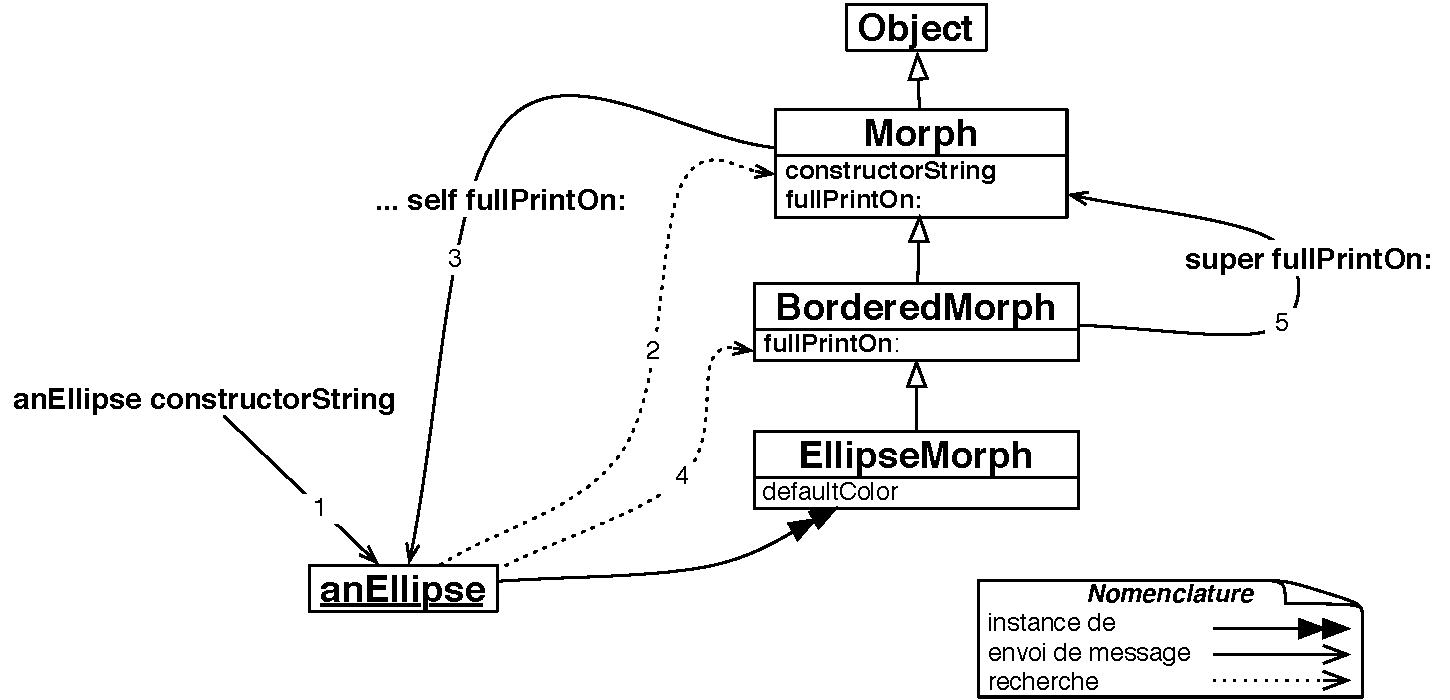
\includegraphics[width=\textwidth]{constructorStringLookup}}
	{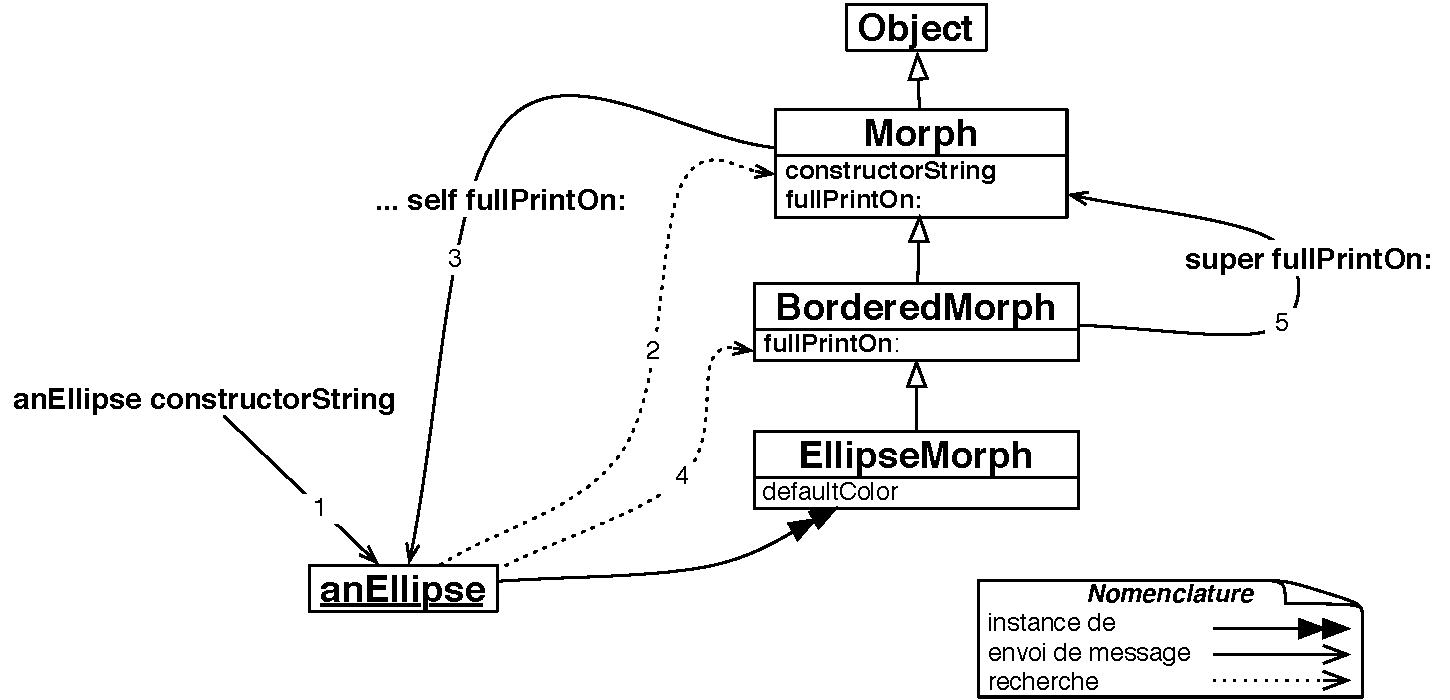
\includegraphics[width=0.8\textwidth]{constructorStringLookup}}
\caption{Les envois à \self et \super.\figlabel{constructorStringLookup}}
\end{center}
\end{figure}

\needlines{2} %CHANGE
\begin{method}[constructorString]{Un envoi à \self}
Morph>>>constructorString
	^ String streamContents: [:s | self printConstructorOn: s indent: 0]
\end{method}

% \arelire{La méthode \cmind{Morph}{constructorString} envoie
%  \ct{printConstructorOn:indent:} à \self.
% Ce message est \arevoir{recherché} dans la hiérarchie en commençant dans la classe
% \lct{EllipseMorph} et finalement trouvé dans \ct{Morph}.}
% This message is also looked up, starting in the class \lct{EllipseMorph}, and found in \ct{Morph}.
% \arelire{Cette méthode en retour envoie à \self le message
% \lct{printConstructorOn:indent:nodeDict:}, qui, à son tour, envoie
% \ct{fullPrintOn:} à \self.
% Encore une fois, \ct{fullPrintOn:} est \arevoir{recherché} depuis la classe
% \ct{EllipseMorph} et \mthind{BorderedMorph}{fullPrintOn:} 
% est trouvé dans \ct{BorderedMorph} 
% (revoir\figref{constructorStringLookup})} % CHANGE

La méthode \cmind{Morph}{constructorString} envoie le message
\ct{printConstructorOn:indent:} à \self. La méthode correspondante à ce
message est alors recherchée dans la hiérarchie de classes d'abord en
en commençant dans la classe \lct{EllipseMorph} et finalement trouvé dans \ct{Morph}.
Cette méthode en retour envoie à \self le message
\lct{printConstructorOn:indent:nodeDict:}, qui, à son tour, envoie
\ct{fullPrintOn:} à \self. Encore une fois, \ct{fullPrintOn:} est recherché
depuis la classe \ct{EllipseMorph} et \mthind{BorderedMorph}{fullPrintOn:} 
est trouvé dans \ct{BorderedMorph} 
(revoir\figref{constructorStringLookup}) % CHANGE
Ce qui est crucial à observer est le fait qu'un envoi à self provoque une recherche de méthode
qui débute dans la classe du receveur, à savoir la classe de anEllipse.

\important{Un envoi à \self déclenche le départ de la recherche \emph{dynamique} de méthode dans la classe du receveur.}

\needlines{4}
\begin{method}[fullPrintOn]{Combiner l'usage de \super et \self}
BorderedMorph>>>fullPrintOn: aStream
	aStream nextPutAll: '('.
	!\emcode{super fullPrintOn: aStream.}!
	aStream nextPutAll: ') setBorderWidth: '; print: borderWidth;
		nextPutAll: ' borderColor: ' , (self colorString: borderColor)
\end{method}
Maintenant, \ct{BorderedMorph>>>fullPrintOn:} utilise l'envoi à \super pour étendre le comportement \ct{fullPrintOn:} hérité de sa super-classe.
Parce qu'il s'agit d'un envoi à \super, la recherche démarre alors
depuis la super-classe de la classe dans laquelle se produit l'envoi à
\super, autrement dit, dans 
\ct{Morph}.
Nous trouvons ainsi immédiatemment \ct{Morph>>>fullPrintOn:} que nous évaluons.

Notez que la recherche sur \super n'a pas commencé dans la 
super-classe du receveur. Ainsi il en aurait résulté
un départ de la recherche depuis \ct{BorderedMorph}, 
créant alors une boucle infinie!

\important{Un envoi à \super déclenche un départ de recherche \emph{statique} de méthode dans la super-classe de la classe dont la méthode envoie le message à \super.}

Si vous regardez attentivement l'envoi à \super et \figref{constructorStringLookup}, vous réaliserez que les liens à \super sont statiques: tout ce qui importe
est la classe dans laquelle le texte de l'envoi à \super est trouvé.
A contrario, le sens de \self est dynamique: \self représente toujours le
receveur du message courant exécuté. Ce qui signifie que  \emph{tout} message envoyé à \self est recherché en partant de la classe du receveur.

%---------------------------------------------------------
\subsection{MessageNotUnderstood}
%\subsection{Message incompris}

Que se passe-t-il si la méthode que nous cherchons n'est pas trouvée?
\index{message!not understood}
%\index{message!incompris}

Supposons que nous envoyons le message \ct{foo} à une ellipse \ct{anEllipse}.
Tout d'abord, la recherche normale de cette méthode aurait à parcourir
toute la chaîne d'héritage jusqu'à la classe \clsind{Object} (ou
plutôt \clsind{ProtoObject}).
Comme cette méthode n'est pas trouvée, la \ind{machine virtuelle} veillera
à ce que l'object envoie \ct{self doesNotUnderstand: #foo}.
(voir \figref{fooNotFound}.)

\begin{figure}[htb]
\begin{center}
\ifluluelse
	{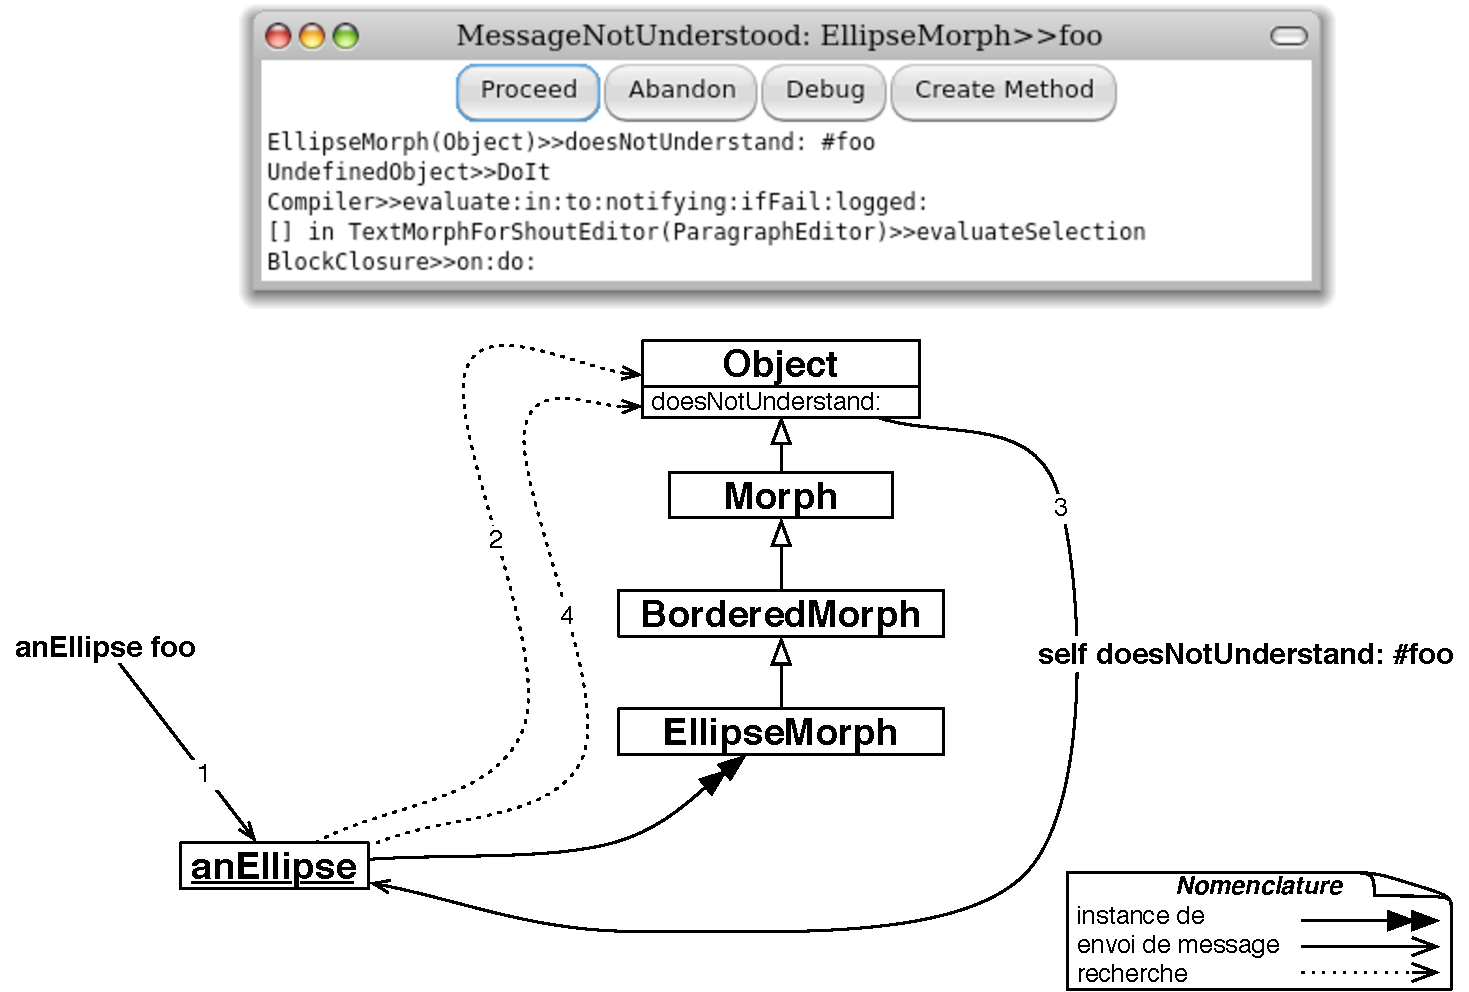
\includegraphics[width=\textwidth]{fooNotFound}}
	{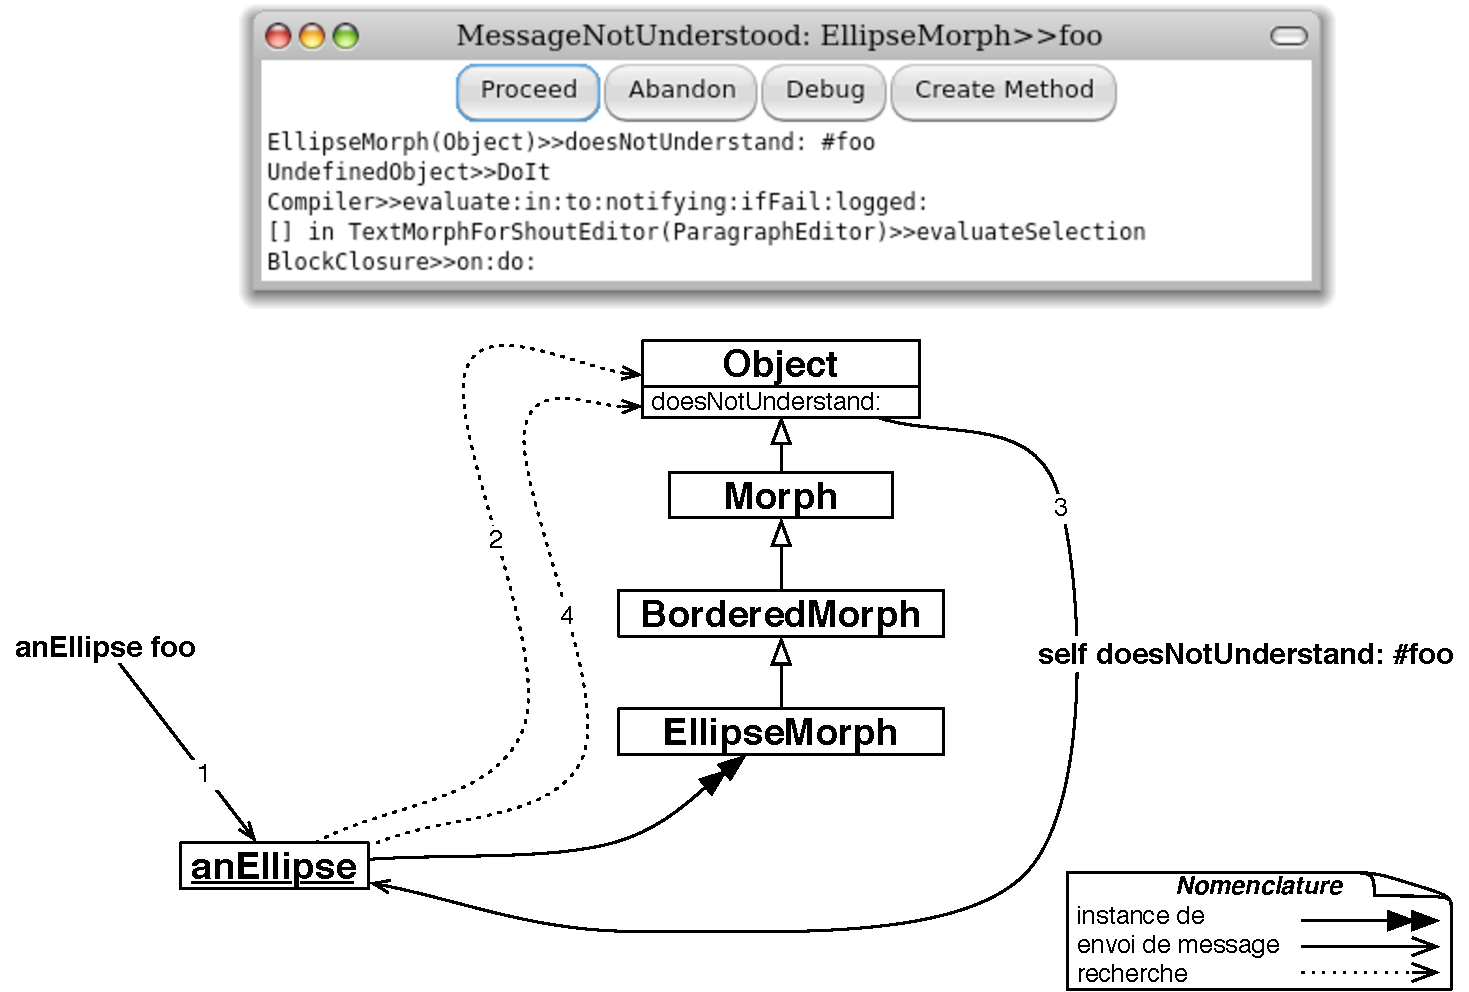
\includegraphics[width=0.8\textwidth]{fooNotFound}}
\caption{Le message \ct{foo} n'est pas compris (not understood).\figlabel{fooNotFound}}
\end{center}
\end{figure}

Ceci est un envoi dynamique de message tout à fait normal. Ainsi
la recherche recommence depuis la classe \ct{EllipseMorph}, mais
cette fois-ci en cherchant la méthode \ct{doesNotUnderstand:}~\footnote{Le nom du message peut se traduire par: \emph{``ne comprend pas''}.}.
Il apparaît que \lct{Object} implémente \ct{doesNotUnderstand:}.
Cette méthode créera un nouvel objet \ct{MessageNotUnderstood} (en français: Message incompréhensible) capable de démarrer Debugger, le débogueur, dans le contexte actuel de l'exécution.

Pourquoi prenons-nous ce chemin sinueux pour gérer une erreur si évidente?
Parce qu'en faisant ainsi, le développeur dispose de tous les outils pour
agir alternativement grâce à l'interception de ces erreurs.
N'importe qui peut surcharger la méthode \mthind{Object}{doesNotUnderstand:} 
dans une sous-classe de \ct{Object} en étendant ses possibilités en
offrant une façon différente de capturer l'erreur.

En fait, nous nous simplifions la vie en implémentant une 
délégation automatique de messages d'un objet à un autre.
Un objet \ct{Delegator} peut simplement déléguer tous les messages
qu'il ne comprend pas à un autre objet dont la responsabilité est de les gérer ou
de lever une erreur lui-même!

%=========================================================
\section{Les variables partagées}

Maintenant, intéressons-nous à un aspect de \st que nous n'avons pas couvert
par nos cinq règles: les variables \subind{variable}{partagée}{}s.

\st offre trois sortes de variables partagées: (1) les variables \emph{globales}; (2) les \emph{variables de classe} partagées entre les instances et les classes, et (3) les variables partagées parmi un groupe de classes ou \emph{variables de pool}.  Les noms de toutes ces variables partagées commencent par une lettre capitale (majuscule), pour nous informer qu'elles sont partagées entre plusieurs objets.
\index{variable!globale}
\index{classe!variable}
\index{variable!pool}

%---------------------------------------------------------
\subsection{Les variables globales}
En \pharo, toutes les variables globales sont stockées dans un espace de nommage appelé \glbind{Smalltalk} qui est une instance de la classe \clsind{SystemDictionary}.
Les variables globales sont accessibles de partout.
Toute classe est nommée par une variable globale; en plus, quelques variables globales sont utilisées pour nommer des objets spéciaux ou couramment utilisés.  

La variable \glbind{Transcript} nomme une instance de \clsind{TranscriptStream}, un flux de données ou \emph{stream} qui écrit dans une fenêtre à ascenseur (dite aussi \emph{scrollable}).
Le code suivant affiche des informations dans le \ct{Transcript} en passant une ligne.

\begin{code}{}
Transcript show: 'Pharo est extra' ; cr
\end{code} % A REVOIR 'Pharo is fun and powerful'

\noindent
Avant de lancer la commande \menu{do it}, ouvrez un Transcript en 
sélectionnant \menu{World \go Tools \ldots \go Transcript}. % CHANGE

\hint{Écrire dans le Transcript est lent, surtout quand la fenêtre Transcript est ouverte. 
Ainsi, si vous constatez un manque de réactivité de votre système alors que vous êtes en train d'écrire dans le Transcript, pensez à le minimiser (bouton \emph{collapse this window}).}

\subsubsection{D'autres variables globales utiles}

\begin{itemize}
\item
\ct{Smalltalk} est une instance de \ct{SystemDictionary} (Dictionnaire Système) définissant toutes les variables globales\,---\,dont l'objet \ct{Smalltalk} lui-même.   
Les clés de ce dictionnaire sont des symboles nommant les objets globaux dans le code \st.
Ainsi par exemple,
\begin{code}{@TEST}
Smalltalk at: #Boolean --> Boolean
\end{code}
Puisque \ct{Smalltalk} est aussi une variable globale lui-même,
\begin{code}{}
Smalltalk at: #Smalltalk-->a SystemDictionary(lots of globals)}
\end{code} 
et
\begin{code}{@TEST}
(Smalltalk at: #Smalltalk) == Smalltalk --> true
\end{code}

\item \clsind{Sensor} est une instance of \clsind{EventSensor}. Il représente les entrées interactives ou interfaces de saisie (en anglais, \emph{input}) dans \pharo. Par exemple, \ct{Sensor keyboard} retourne le caractère suivant saisi au clavier, et \ct{Sensor leftShiftDown} répond \ct{true} (vrai en booléen) si la touche \emph{shift} gauche est maintenue enfoncée, alors que \ct{Sensor mousePoint} renvoie un \ct{Point} indiquant la position actuelle de la souris.

\item \glbind{World} (Monde en anglais) est une instance de \clsind{PasteUpMorph} représentant l'écran.
\ct{World bounds} retourne un rectangle définissant l'espace tout entier de l'écran; tous les morphs (objet Morph) sur l'écran sont des sous-morphs ou \emph{submorphs} de \ct{World}.
\index{Morphic}

\item \glbind{ActiveHand} est l'instance courante de \clsind{HandMorph}, la représentation graphique du curseur. Les sous-morphs de \ct{ActiveHand} tiennent tout ce qui est glissé par la souris.
\ab{I have never used this, and had to browse the image to see what it is!  What do you use it for?}

\item
\glbind{Undeclared}~\footnote{Non déclaré, en français.} est un autre dictionnaire\,---\,il contient toutes les variables non déclarées.
Si vous écrivez une méthode qui référence une variable non déclarée,
le navigateur de classe (Browser) vous l'annoncera normalement
pour que vous la déclariez, par exemple, en tant que variable globale ou variable d'instance de la classe.
Cependant, si par la suite, vous effacez la déclaration, le code référencera une variable non déclarée. 
Inspecter \ct{Undeclared} peut parfois expliquer des comportements bizarres!

\item
\glbind{SystemOrganization} est une instance de
\clsind{SystemOrganizer}: il enregistre l'organisation des classes en
paquets.  Plus précisement, il catégorise les \emph{noms} des
classes, ainsi
\end{itemize} %CHANGE
\begin{code}{@TEST}
SystemOrganization categoryOfElement: #Magnitude --> #'Kernel-Numbers'
\end{code}
%\end{itemize} % CHANGE dans PBE, c'est \end{itemize} du dessus qui
               % prend le relais

Une pratique courante est de limiter fortement l'usage des variables globales;
il est toujours préférable d'utiliser des variables d'instance de classe ou des variables de classes et de fournir des méthodes de classe pour y accéder.
En effet, si aujourd'hui \pharo devait être reprogrammé à partir de
zéro~\footnote{Le terme anglais est: \emph{from scratch}, signifiant depuis le début.}, la plupart des variables globales qui ne sont pas des classes seraient remplacées par des Singletons.

La technique habituellement employée pour définir une variable globale
est simplement de faire un \menu{do it} sur une affectation d'un identifiant
non déclaré commençant par une majuscule. Dès lors,
l'analyseur syntaxique ou \emph{parser} vous 
la déclarera en tant que variable globale.  
Si vous voulez en définir une de manière programmatique, exécutez
\ct{Smalltalk at: #AGlobalName put: nil}.
Pour l'effacer, exécutez \ct{Smalltalk removeKey: #AGlobalName}.
\glbindex{Smalltalk}

%---------------------------------------------------------
\subsection{Les variables de classe}
\seclabel{classVars}

Nous avons besoin parfois de partager des données entre les instances d'une classe et la classe elle-même.
C'est possible grâce aux \emph{variables de classe}. 
Le terme \subind{classe}{variable} de classe indique que le cycle de vie
de la variable est le même que celui de la classe. Cependant, 
le terme ne véhicule pas l'idée que ces variables sont partagées aussi bien parmi toutes
les instances d'une classe que dans la classe elle-même comme nous pouvons le voir sur \figref{privateSharedVar}.
En fait, \emph{variables partagées} (ou \emph{shared variables}, en anglais) aurait
été un meilleur nom car ce dernier exprime plus clairement leur rôle
tout en pointant le danger de les utiliser, en particulier si elles sont 
sujettes aux modifications.

\begin{figure}[htb]
\begin{center}
\ifluluelse
	{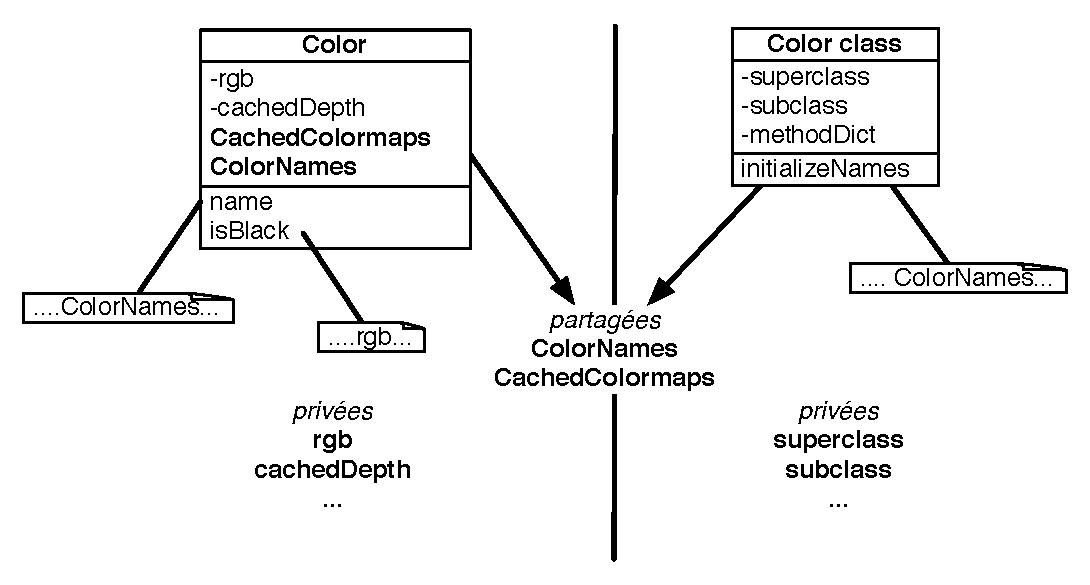
\includegraphics[width=\textwidth]{privateSharedVarColor}}
	{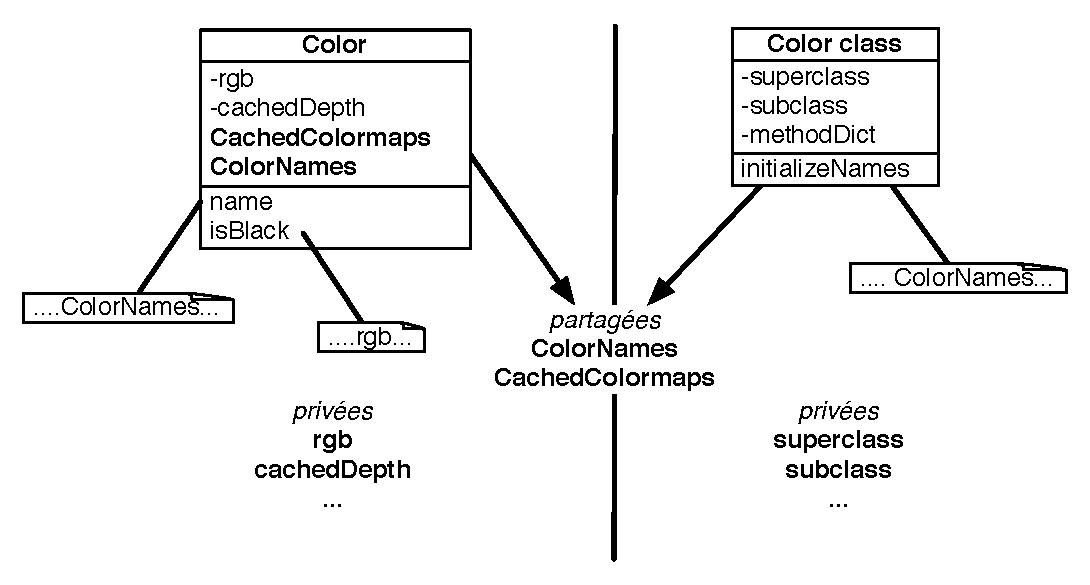
\includegraphics[width=0.7\textwidth]{privateSharedVarColor}}
\caption{Des méthodes d'instance et de classe accédant à différentes
variables.\figlabel{privateSharedVar}}
\end{center}
\end{figure}

Sur \figref{privateSharedVar} nous voyons que \ct{rgb} et \ct{cachedDepth} sont
des variables d'instance de \ct{Color} uniquement accessibles par les 
instances de \clsind{Color}.
Nous remarquons aussi que \ct{superclass}, \ct{subclass}, \ct{methodDict}\ldots \etc, sont des variables d'instance de classe, \ie des variables d'instance  accessibles seulement par \ct{Color} class.

Mais nous pouvons noter quelque chose de nouveau: \ct{ColorNames} et \ct{CachedColormaps} sont des \emph{variables de classe} définies pour \ct{Color}.
La capitalisation du nom de ces variables nous donne un indice sur le fait qu'elles sont partagées.
En fait, non seulement toutes les instances de \ct{Color} peuvent accéder
à ces variables partagées, mais aussi la classe \ct{Color} elle-même, ainsi que \emph{toutes ses sous-classes}.
Les méthodes d'instance et de classe peuvent accéder toutes les deux
à ces variables partagées.

%\begin{figure}
%\begin{center}\includegraphics[width=6cm]{dateToday}\caption{A date is an object that  represents only anumber of days; all the information about month names, day names, etc.\ is shared among all the instances \figlabel{dateToday}}\end{center}.
%\end{figure}

Une \subind{classe}{variable} de classe est déclarée dans le patron de définition de la classe.
Par exemple, la classe \ct{Color} définit un grand nombre de variables de classe pour accélérer la création des couleurs;
sa définition est visible ci-dessous (\clsref{Color}).

\needlines{5} % CHANGE
\begin{classdef}[Color]{Color et ces variables de classe}
Object subclass: #Color 	
        instanceVariableNames: 'rgb cachedDepth cachedBitPattern'
        classVariableNames: 'Black Blue BlueShift Brown CachedColormaps ColorChart ColorNames ComponentMask ComponentMax Cyan DarkGray Gray GrayToIndexMap Green GreenShift HalfComponentMask HighLightBitmaps IndexedColors LightBlue LightBrown LightCyan LightGray LightGreen LightMagenta LightOrange LightRed LightYellow Magenta MaskingMap Orange PaleBlue PaleBuff PaleGreen PaleMagenta PaleOrange PalePeach PaleRed PaleTan PaleYellow PureBlue PureCyan PureGreen PureMagenta PureRed PureYellow RandomStream Red RedShift TranslucentPatterns Transparent VeryDarkGray VeryLightGray VeryPaleRed VeryVeryDarkGray VeryVeryLightGray White Yellow'
        poolDictionaries: '' 	
        category: 'Graphics-Primitives'
\end{classdef}

La variable de classe \cvind{ColorNames} est un tableau contenant le nom des couleurs fréquemment utilisées. Ce tableau est partagé par toutes les instances de \ct{Color} et de sa sous-classe \clsind{TranslucentColor}. 
Elles sont accessibles via les méthodes d'instance et de classe.

% (see \figref{ClassVarAccess2}).

\ct{ColorNames} est initialisée une fois dans \cmind{Color class}{initializeNames}, mais elle est en libre accès depuis les instances de \ct{Color}.
La méthode \cmind{Color}{name} utilise la variable pour trouver
le nom de la couleur.
Il semble en effet inopportun d'ajouter une variable d'instance \ct{name}
à chaque couleur car la plupart des couleurs n'ont pas de noms.
 
\subsubsection{L'initialisation de classe}

La présence de variables de classe soulève une question: comment les initialiser?

Une solution est l'\subind{classe}{initialisation} dite paresseuse (ou \emph{lazy initialization} en anglais).
Cela est possible avec l'introduction d'une méthode d'\subind{méthode}{accès} qui
initialise la variable, durant l'exécution, si celle-ci n'a pas été
encore initialisée.
Ceci nous oblige à utiliser la méthode d'accès tout le temps et à ne jamais
faire appel à la variable de classe directement.
De plus, notons que le coût de l'envoi d'un accesseur et le test d'initialisation sont à prendre en compte.
Ceci va à l'encontre de notre motivation à utiliser une variable de classe, parce qu'en réalité elle n'est plus partagée.

\begin{method}[colorclasscolornames]{\ct{Color class>>>colorNames}}
Color class>>>colorNames	
	ColorNames ifNil: [self initializeNames].
	^ ColorNames
\end{method}	
\cmindex{Color class}{colorNames}

Une autre solution consiste à surcharger la méthode \ct{initialize}.

\needlines{3}
\begin{method}[colorclassinit]{\ct{Color class>>>initialize}}
Color class>>>initialize	
	!\ldots!
	self initializeNames
\end{method}
\cmindex{Color class}{initialize}

\noindent
Si vous adoptez cette solution, vous devez vous rappeler qu'il faut
invoquer la méthode \ct{initialize} après que vous l'ayez définie,
\eg en utilisant \ct{Color initialize}.
Bien que les méthodes \subind{Browser}{côté classe} \ct{initialize} soient exécutées automatiquement lorsque le code est chargé en mémoire,
elles ne sont \emph{pas} exécutées durant leur saisie et leur compilation dans le navigateur Browser ou en phase d'édition et de recompilation.

%---------------------------------------------------------
\subsection{Les variables de pool}
Les variables de \emph{pool}~\footnote{Pool signifie piscine en anglais, ces variables sont dans un même bain!} sont des variables qui sont partagées entre plusieurs classes qui ne sont pas liées par une arborescence d'héritage.
à la base, les variables de pool sont stockées dans des dictionnaires
de pool;  maintenant elles devraient être définies comme variables
de classe dans des classes dédiées (sous-classes de SharedPool).
Notre conseil: évitez-les. Vous n'en aurez besoin qu'en des circonstances
exceptionnelles et spécifiques.
Ici, notre but est de vous expliquer suffisamment les variables de
\subind{variable}{pool} pour comprendre leur fonction quand vous les
rencontrez durant la lecture de code.

Une classe qui accède à une variable de pool doit mentionner le \emph{pool}
dans sa définition de classe.
Par exemple, la classe \clsind{Text} indique qu'elle emploie le dictionnaire
de pool \ct{TextConstants} qui contient toutes les constantes textuelles
telles que 
\glbind{CR} and \glbind{LF}. 
Ce dictionnaire a une clé \ct{#CR} à laquelle est affectée la valeur
\ct{Character cr}, \ie le caractère retour-chariot ou \emph{carriage return}.
\cmindex{Character class}{cr}

\begin{classdef}[textpooldict]{Dictionnaire de pool dans la classe \ct{Text}}
ArrayedCollection subclass: #Text
        instanceVariableNames: 'string runs' 	
        classVariableNames: '' 	
        !\emcode{poolDictionaries: 'TextConstants'}!
        category: 'Collections-Text'
\end{classdef}
   
Ceci permet aux méthodes de la classe \ct{Text} d'accéder aux clés
du dictionnaire \emph{directement} dans le corps de la méthode, \ie 
en utilisant la syntaxe de variable plutôt qu'une recherche explicite
dans le dictionnaire.
Par exemple, nous pouvons écrire la méthode suivante.

\needlines{3}
\begin{method}[texttestcr]{\ct{Text>>>testCR}}
Text>>>testCR 	
      ^ CR == Character cr
\end{method}

Encore une fois, nous recommandons d'éviter d'utiliser
les variables et les dictionnaires de pool.

%=========================================================
\section{Résumé du chapitre}

Le modèle objet de \pharo est à la fois simple et uniforme.
\Mantra et quasiment tout se passe via l'envoi de messages. % REVOIR
                                % 'by sending messages'

\begin{itemize}

\item \Mantra.
  Les entités primitives telles que les entiers sont des objets, ainsi que les classes qui sont des objets comme les autres.

\item Tout objet est instance d'une classe.
Les classes définissent la structure de leurs instances via des
variables d'instance \emph{privées} et leur comportement 
via des méthodes \emph{publiques}. Chaque classe est l'unique
instance de sa méta-classe.
Les variables de classe sont des variables privées partagées par la classe
et toutes les instances de la classe.
Les classes ne peuvent pas accéder directement aux variables d'instance de
leurs instances et les instances ne peuvent pas accéder aux variables de
classe de leur classe.
Les méthodes d'\subind{méthode}{accès} (accesseurs et mutateurs) doivent être
définies au besoin.  

  \item Toute classe a une super-classe.
  La racine de la hiérarchie basée sur l'héritage simple est \ct{ProtoObject}.
	Cependant les classes que vous définissez devrait normalement hériter de la classe \ct{Object} ou de ses sous-classes.
Il n'y a pas d'élément sémantique pour la définition de classes abstraites.
Une classe abstraite est simplement une classe avec au moins une méthode abstraite
\,---\,une dont l'implémentation contient l'expression 
\ct{self subclassResponsibility}.
  Bien que \pharo ne dispose que du principe d'héritage simple, 
il est facile de partager les implémentations de méthodes
en regroupant ces dernières en \emph{traits}.

  \item Tout se passe par envoi de messages. % REVOIR 'by sending
                                             % messages'

	Nous ne faisons pas des ``appels de méthodes'', nous faisons des ``envois de messages''.
        Le receveur choisit alors sa propre méthode pour répondre au message.

  \item La recherche de méthodes suit la chaîne d'héritage;
        Les envois à \self sont dynamiques et la recherche de méthode
        démarre dans le receveur de la classe, alors que
        celles à \super sont statiques et la recherche commence dans la super-classe de la 
        classe dans laquelle l'envoi à \super est écrit.

  \item Il y a trois sortes de variables partagées.
        Les variables globales sont accessibles partout dans le système.
        Les variables de classe sont partagées entre une classe, ses sous-classes et ses instances.
        Les variables de pool sont partagées dans un ensemble de classes particulier.
        Vous devez éviter l'emploi de variables partagées autant que possible.

\end{itemize}

%=========================================================
\ifx\wholebook\relax\else
   \bibliographystyle{jurabib}
   \nobibliography{scg}
   \end{document}
\fi
%=========================================================

%=================================================================
%%% Local Variables:
%%% coding: utf-8
%%% mode: latex
%%% TeX-master: t
%%% TeX-PDF-mode: t
%%% End:

%---------------------------------------------------------
